\documentclass[twoside]{book}

% Packages required by doxygen
\usepackage{calc}
\usepackage{doxygen}
\usepackage{graphicx}
\usepackage[utf8]{inputenc}
\usepackage{makeidx}
\usepackage{multicol}
\usepackage{multirow}
\usepackage{textcomp}
\usepackage[table]{xcolor}

% Font selection
\usepackage[T1]{fontenc}
\usepackage{mathptmx}
\usepackage[scaled=.90]{helvet}
\usepackage{courier}
\usepackage{amssymb}
\usepackage{sectsty}
\renewcommand{\familydefault}{\sfdefault}
\allsectionsfont{%
  \fontseries{bc}\selectfont%
  \color{darkgray}%
}
\renewcommand{\DoxyLabelFont}{%
  \fontseries{bc}\selectfont%
  \color{darkgray}%
}

% Page & text layout
\usepackage{geometry}
\geometry{%
  a4paper,%
  top=2.5cm,%
  bottom=2.5cm,%
  left=2.5cm,%
  right=2.5cm%
}
\tolerance=750
\hfuzz=15pt
\hbadness=750
\setlength{\emergencystretch}{15pt}
\setlength{\parindent}{0cm}
\setlength{\parskip}{0.2cm}
\makeatletter
\renewcommand{\paragraph}{%
  \@startsection{paragraph}{4}{0ex}{-1.0ex}{1.0ex}{%
    \normalfont\normalsize\bfseries\SS@parafont%
  }%
}
\renewcommand{\subparagraph}{%
  \@startsection{subparagraph}{5}{0ex}{-1.0ex}{1.0ex}{%
    \normalfont\normalsize\bfseries\SS@subparafont%
  }%
}
\makeatother

% Headers & footers
\usepackage{fancyhdr}
\pagestyle{fancyplain}
\fancyhead[LE]{\fancyplain{}{\bfseries\thepage}}
\fancyhead[CE]{\fancyplain{}{}}
\fancyhead[RE]{\fancyplain{}{\bfseries\leftmark}}
\fancyhead[LO]{\fancyplain{}{\bfseries\rightmark}}
\fancyhead[CO]{\fancyplain{}{}}
\fancyhead[RO]{\fancyplain{}{\bfseries\thepage}}
\fancyfoot[LE]{\fancyplain{}{}}
\fancyfoot[CE]{\fancyplain{}{}}
\fancyfoot[RE]{\fancyplain{}{\bfseries\scriptsize Generated on Thu Nov 20 2014 22\-:29\-:44 for A\-S\-T by Doxygen }}
\fancyfoot[LO]{\fancyplain{}{\bfseries\scriptsize Generated on Thu Nov 20 2014 22\-:29\-:44 for A\-S\-T by Doxygen }}
\fancyfoot[CO]{\fancyplain{}{}}
\fancyfoot[RO]{\fancyplain{}{}}
\renewcommand{\footrulewidth}{0.4pt}
\renewcommand{\chaptermark}[1]{%
  \markboth{#1}{}%
}
\renewcommand{\sectionmark}[1]{%
  \markright{\thesection\ #1}%
}

% Indices & bibliography
\usepackage{natbib}
\usepackage[titles]{tocloft}
\setcounter{tocdepth}{3}
\setcounter{secnumdepth}{5}
\makeindex

% Hyperlinks (required, but should be loaded last)
\usepackage{ifpdf}
\ifpdf
  \usepackage[pdftex,pagebackref=true]{hyperref}
\else
  \usepackage[ps2pdf,pagebackref=true]{hyperref}
\fi
\hypersetup{%
  colorlinks=true,%
  linkcolor=blue,%
  citecolor=blue,%
  unicode%
}

% Custom commands
\newcommand{\clearemptydoublepage}{%
  \newpage{\pagestyle{empty}\cleardoublepage}%
}


%===== C O N T E N T S =====

\begin{document}

% Titlepage & ToC
\hypersetup{pageanchor=false}
\pagenumbering{roman}
\begin{titlepage}
\vspace*{7cm}
\begin{center}%
{\Large A\-S\-T }\\
\vspace*{1cm}
{\large Generated by Doxygen 1.8.6}\\
\vspace*{0.5cm}
{\small Thu Nov 20 2014 22:29:44}\\
\end{center}
\end{titlepage}
\clearemptydoublepage
\tableofcontents
\clearemptydoublepage
\pagenumbering{arabic}
\hypersetup{pageanchor=true}

%--- Begin generated contents ---
\chapter{A\-S\-T Used to Parse F\-C\-A\-L Language and Covert it to C++}
\label{index}\hypertarget{index}{}\hypertarget{index_Introduction}{}\section{Introduction}\label{index_Introduction}
In this \hyperlink{AST_8h_source}{A\-S\-T.\-h} file, we define the context free grammar used to parse the F\-C\-A\-L language. We use inheritance and virtual classes to define productions in the grammar, and concrete subclasses of the virtual classes to define the terminals.\hypertarget{index_How}{}\section{to Use}\label{index_How}
Navigate to the currently working directory (the one that this file is stored in) in the terminal, then simply type \char`\"{}make run-\/tests\char`\"{}. This will compile the translator and execute the cxxtests defined in \hyperlink{regex__tests_8h_source}{regex\-\_\-tests.\-h}, \hyperlink{scanner__tests_8h_source}{scanner\-\_\-tests.\-h}, \hyperlink{parser__tests_8h_source}{parser\-\_\-tests.\-h}, and \hyperlink{AST__tests_8h_source}{A\-S\-T\-\_\-tests.\-h}. Once Iteration 4 is complete, there will be a way to execute the program on a specific file, to be inputted by the user. 
\chapter{Hierarchical Index}
\section{Class Hierarchy}
This inheritance list is sorted roughly, but not completely, alphabetically\-:\begin{DoxyCompactList}
\item \contentsline{section}{Ext\-Token}{\pageref{classExtToken}}{}
\begin{DoxyCompactList}
\item \contentsline{section}{Char\-Const\-Token}{\pageref{classCharConstToken}}{}
\item \contentsline{section}{Dash\-Token}{\pageref{classDashToken}}{}
\item \contentsline{section}{End\-Of\-File\-Token}{\pageref{classEndOfFileToken}}{}
\item \contentsline{section}{False\-Kwd\-Token}{\pageref{classFalseKwdToken}}{}
\item \contentsline{section}{Float\-Const\-Token}{\pageref{classFloatConstToken}}{}
\item \contentsline{section}{Forward\-Slash\-Token}{\pageref{classForwardSlashToken}}{}
\item \contentsline{section}{If\-Token}{\pageref{classIfToken}}{}
\item \contentsline{section}{Int\-Const\-Token}{\pageref{classIntConstToken}}{}
\item \contentsline{section}{Left\-Paren\-Token}{\pageref{classLeftParenToken}}{}
\item \contentsline{section}{Let\-Token}{\pageref{classLetToken}}{}
\item \contentsline{section}{Not\-Op\-Token}{\pageref{classNotOpToken}}{}
\item \contentsline{section}{Plus\-Sign\-Token}{\pageref{classPlusSignToken}}{}
\item \contentsline{section}{Relational\-Op\-Token}{\pageref{classRelationalOpToken}}{}
\item \contentsline{section}{Star\-Token}{\pageref{classStarToken}}{}
\item \contentsline{section}{String\-Const\-Token}{\pageref{classStringConstToken}}{}
\item \contentsline{section}{True\-Kwd\-Token}{\pageref{classTrueKwdToken}}{}
\item \contentsline{section}{Variable\-Name\-Token}{\pageref{classVariableNameToken}}{}
\end{DoxyCompactList}
\item \contentsline{section}{mysequence$<$ T, N $>$}{\pageref{classmysequence}}{}
\item \contentsline{section}{Node}{\pageref{classNode}}{}
\begin{DoxyCompactList}
\item \contentsline{section}{Expr}{\pageref{classExpr}}{}
\begin{DoxyCompactList}
\item \contentsline{section}{Expr\-Bin\-Op}{\pageref{classExprBinOp}}{}
\item \contentsline{section}{Expr\-Bool}{\pageref{classExprBool}}{}
\item \contentsline{section}{Expr\-Const\-Float}{\pageref{classExprConstFloat}}{}
\item \contentsline{section}{Expr\-Const\-Int}{\pageref{classExprConstInt}}{}
\item \contentsline{section}{Expr\-Const\-Str}{\pageref{classExprConstStr}}{}
\item \contentsline{section}{Expr\-Last}{\pageref{classExprLast}}{}
\item \contentsline{section}{Expr\-Matrix\-Ref}{\pageref{classExprMatrixRef}}{}
\item \contentsline{section}{Expr\-Nested}{\pageref{classExprNested}}{}
\item \contentsline{section}{Expr\-Var}{\pageref{classExprVar}}{}
\item \contentsline{section}{If\-Expr}{\pageref{classIfExpr}}{}
\item \contentsline{section}{Let\-Expr}{\pageref{classLetExpr}}{}
\item \contentsline{section}{Not\-Expr}{\pageref{classNotExpr}}{}
\item \contentsline{section}{Varname}{\pageref{classVarname}}{}
\end{DoxyCompactList}
\item \contentsline{section}{Root}{\pageref{classRoot}}{}
\item \contentsline{section}{Stmt}{\pageref{classStmt}}{}
\begin{DoxyCompactList}
\item \contentsline{section}{Decl}{\pageref{classDecl}}{}
\begin{DoxyCompactList}
\item \contentsline{section}{Decl\-Matrix\-One}{\pageref{classDeclMatrixOne}}{}
\item \contentsline{section}{Decl\-Matrix\-Two}{\pageref{classDeclMatrixTwo}}{}
\item \contentsline{section}{Kwd\-Decl}{\pageref{classKwdDecl}}{}
\end{DoxyCompactList}
\item \contentsline{section}{Stmt\-Asg}{\pageref{classStmtAsg}}{}
\item \contentsline{section}{Stmt\-Curly}{\pageref{classStmtCurly}}{}
\item \contentsline{section}{Stmt\-Empty}{\pageref{classStmtEmpty}}{}
\item \contentsline{section}{Stmt\-For}{\pageref{classStmtFor}}{}
\item \contentsline{section}{Stmt\-If}{\pageref{classStmtIf}}{}
\item \contentsline{section}{Stmt\-If\-Else}{\pageref{classStmtIfElse}}{}
\item \contentsline{section}{Stmt\-Print}{\pageref{classStmtPrint}}{}
\item \contentsline{section}{Stmt\-While}{\pageref{classStmtWhile}}{}
\end{DoxyCompactList}
\item \contentsline{section}{Stmts}{\pageref{classStmts}}{}
\begin{DoxyCompactList}
\item \contentsline{section}{Empty\-Stmts}{\pageref{classEmptyStmts}}{}
\item \contentsline{section}{Stmts\-Seq}{\pageref{classStmtsSeq}}{}
\end{DoxyCompactList}
\end{DoxyCompactList}
\item \contentsline{section}{Parser}{\pageref{classParser}}{}
\item \contentsline{section}{Parse\-Result}{\pageref{classParseResult}}{}
\item \contentsline{section}{Scanner}{\pageref{classScanner}}{}
\item Test\-Suite\begin{DoxyCompactList}
\item \contentsline{section}{Parser\-Test\-Suite}{\pageref{classParserTestSuite}}{}
\item \contentsline{section}{Regex\-Test\-Suite}{\pageref{classRegexTestSuite}}{}
\item \contentsline{section}{Scanner\-Test\-Suite}{\pageref{classScannerTestSuite}}{}
\item \contentsline{section}{Scanner\-Test\-Suite}{\pageref{classScannerTestSuite}}{}
\end{DoxyCompactList}
\item \contentsline{section}{Token}{\pageref{classToken}}{}
\end{DoxyCompactList}

\chapter{Class Index}
\section{Class List}
Here are the classes, structs, unions and interfaces with brief descriptions\-:\begin{DoxyCompactList}
\item\contentsline{section}{\hyperlink{classCharConstToken}{Char\-Const\-Token} }{\pageref{classCharConstToken}}{}
\item\contentsline{section}{\hyperlink{classDashToken}{Dash\-Token} }{\pageref{classDashToken}}{}
\item\contentsline{section}{\hyperlink{classDecl}{Decl} }{\pageref{classDecl}}{}
\item\contentsline{section}{\hyperlink{classDeclMatrixOne}{Decl\-Matrix\-One} }{\pageref{classDeclMatrixOne}}{}
\item\contentsline{section}{\hyperlink{classDeclMatrixTwo}{Decl\-Matrix\-Two} }{\pageref{classDeclMatrixTwo}}{}
\item\contentsline{section}{\hyperlink{classEmptyStmts}{Empty\-Stmts} }{\pageref{classEmptyStmts}}{}
\item\contentsline{section}{\hyperlink{classEndOfFileToken}{End\-Of\-File\-Token} }{\pageref{classEndOfFileToken}}{}
\item\contentsline{section}{\hyperlink{classExpr}{Expr} }{\pageref{classExpr}}{}
\item\contentsline{section}{\hyperlink{classExprBinOp}{Expr\-Bin\-Op} }{\pageref{classExprBinOp}}{}
\item\contentsline{section}{\hyperlink{classExprBool}{Expr\-Bool} }{\pageref{classExprBool}}{}
\item\contentsline{section}{\hyperlink{classExprConstFloat}{Expr\-Const\-Float} }{\pageref{classExprConstFloat}}{}
\item\contentsline{section}{\hyperlink{classExprConstInt}{Expr\-Const\-Int} }{\pageref{classExprConstInt}}{}
\item\contentsline{section}{\hyperlink{classExprConstStr}{Expr\-Const\-Str} }{\pageref{classExprConstStr}}{}
\item\contentsline{section}{\hyperlink{classExprLast}{Expr\-Last} }{\pageref{classExprLast}}{}
\item\contentsline{section}{\hyperlink{classExprMatrixRef}{Expr\-Matrix\-Ref} }{\pageref{classExprMatrixRef}}{}
\item\contentsline{section}{\hyperlink{classExprNested}{Expr\-Nested} }{\pageref{classExprNested}}{}
\item\contentsline{section}{\hyperlink{classExprVar}{Expr\-Var} }{\pageref{classExprVar}}{}
\item\contentsline{section}{\hyperlink{classExtToken}{Ext\-Token} }{\pageref{classExtToken}}{}
\item\contentsline{section}{\hyperlink{classFalseKwdToken}{False\-Kwd\-Token} }{\pageref{classFalseKwdToken}}{}
\item\contentsline{section}{\hyperlink{classFloatConstToken}{Float\-Const\-Token} }{\pageref{classFloatConstToken}}{}
\item\contentsline{section}{\hyperlink{classForwardSlashToken}{Forward\-Slash\-Token} }{\pageref{classForwardSlashToken}}{}
\item\contentsline{section}{\hyperlink{classIfExpr}{If\-Expr} }{\pageref{classIfExpr}}{}
\item\contentsline{section}{\hyperlink{classIfToken}{If\-Token} }{\pageref{classIfToken}}{}
\item\contentsline{section}{\hyperlink{classIntConstToken}{Int\-Const\-Token} }{\pageref{classIntConstToken}}{}
\item\contentsline{section}{\hyperlink{classKwdDecl}{Kwd\-Decl} }{\pageref{classKwdDecl}}{}
\item\contentsline{section}{\hyperlink{classLeftParenToken}{Left\-Paren\-Token} }{\pageref{classLeftParenToken}}{}
\item\contentsline{section}{\hyperlink{classLetExpr}{Let\-Expr} }{\pageref{classLetExpr}}{}
\item\contentsline{section}{\hyperlink{classLetToken}{Let\-Token} }{\pageref{classLetToken}}{}
\item\contentsline{section}{\hyperlink{classmysequence}{mysequence$<$ T, N $>$} }{\pageref{classmysequence}}{}
\item\contentsline{section}{\hyperlink{classNode}{Node} }{\pageref{classNode}}{}
\item\contentsline{section}{\hyperlink{classNotExpr}{Not\-Expr} }{\pageref{classNotExpr}}{}
\item\contentsline{section}{\hyperlink{classNotOpToken}{Not\-Op\-Token} }{\pageref{classNotOpToken}}{}
\item\contentsline{section}{\hyperlink{classParser}{Parser} }{\pageref{classParser}}{}
\item\contentsline{section}{\hyperlink{classParseResult}{Parse\-Result} }{\pageref{classParseResult}}{}
\item\contentsline{section}{\hyperlink{classParserTestSuite}{Parser\-Test\-Suite} }{\pageref{classParserTestSuite}}{}
\item\contentsline{section}{\hyperlink{classPlusSignToken}{Plus\-Sign\-Token} }{\pageref{classPlusSignToken}}{}
\item\contentsline{section}{\hyperlink{classRegexTestSuite}{Regex\-Test\-Suite} }{\pageref{classRegexTestSuite}}{}
\item\contentsline{section}{\hyperlink{classRelationalOpToken}{Relational\-Op\-Token} }{\pageref{classRelationalOpToken}}{}
\item\contentsline{section}{\hyperlink{classRoot}{Root} }{\pageref{classRoot}}{}
\item\contentsline{section}{\hyperlink{classScanner}{Scanner} }{\pageref{classScanner}}{}
\item\contentsline{section}{\hyperlink{classScannerTestSuite}{Scanner\-Test\-Suite} }{\pageref{classScannerTestSuite}}{}
\item\contentsline{section}{\hyperlink{classStarToken}{Star\-Token} }{\pageref{classStarToken}}{}
\item\contentsline{section}{\hyperlink{classStmt}{Stmt} }{\pageref{classStmt}}{}
\item\contentsline{section}{\hyperlink{classStmtAsg}{Stmt\-Asg} }{\pageref{classStmtAsg}}{}
\item\contentsline{section}{\hyperlink{classStmtCurly}{Stmt\-Curly} }{\pageref{classStmtCurly}}{}
\item\contentsline{section}{\hyperlink{classStmtEmpty}{Stmt\-Empty} }{\pageref{classStmtEmpty}}{}
\item\contentsline{section}{\hyperlink{classStmtFor}{Stmt\-For} }{\pageref{classStmtFor}}{}
\item\contentsline{section}{\hyperlink{classStmtIf}{Stmt\-If} }{\pageref{classStmtIf}}{}
\item\contentsline{section}{\hyperlink{classStmtIfElse}{Stmt\-If\-Else} }{\pageref{classStmtIfElse}}{}
\item\contentsline{section}{\hyperlink{classStmtPrint}{Stmt\-Print} }{\pageref{classStmtPrint}}{}
\item\contentsline{section}{\hyperlink{classStmts}{Stmts} }{\pageref{classStmts}}{}
\item\contentsline{section}{\hyperlink{classStmtsSeq}{Stmts\-Seq} }{\pageref{classStmtsSeq}}{}
\item\contentsline{section}{\hyperlink{classStmtWhile}{Stmt\-While} }{\pageref{classStmtWhile}}{}
\item\contentsline{section}{\hyperlink{classStringConstToken}{String\-Const\-Token} }{\pageref{classStringConstToken}}{}
\item\contentsline{section}{\hyperlink{classToken}{Token} }{\pageref{classToken}}{}
\item\contentsline{section}{\hyperlink{classTrueKwdToken}{True\-Kwd\-Token} }{\pageref{classTrueKwdToken}}{}
\item\contentsline{section}{\hyperlink{classVariableNameToken}{Variable\-Name\-Token} }{\pageref{classVariableNameToken}}{}
\item\contentsline{section}{\hyperlink{classVarname}{Varname} }{\pageref{classVarname}}{}
\end{DoxyCompactList}

\chapter{Class Documentation}
\hypertarget{classCharConstToken}{\section{Char\-Const\-Token Class Reference}
\label{classCharConstToken}\index{Char\-Const\-Token@{Char\-Const\-Token}}
}
Inheritance diagram for Char\-Const\-Token\-:\begin{figure}[H]
\begin{center}
\leavevmode
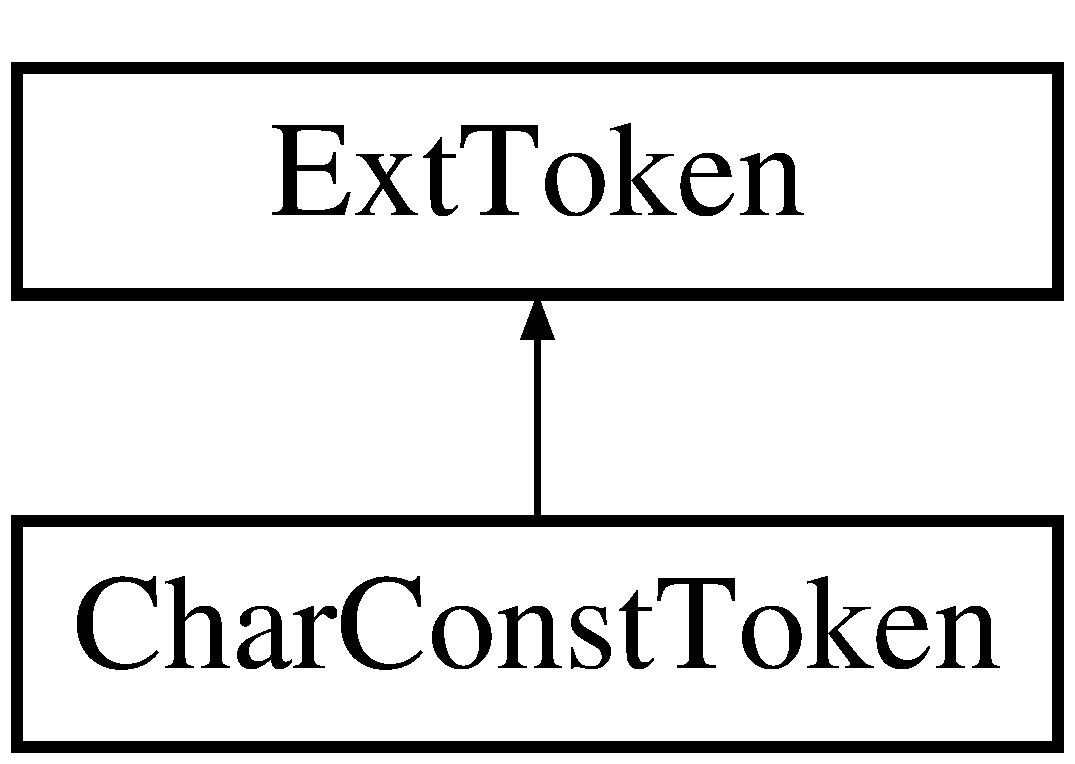
\includegraphics[height=2.000000cm]{classCharConstToken}
\end{center}
\end{figure}
\subsection*{Public Member Functions}
\begin{DoxyCompactItemize}
\item 
\hypertarget{classCharConstToken_a9dcb8d0d26c4f9c66570357641933c51}{{\bfseries Char\-Const\-Token} (\hyperlink{classParser}{Parser} $\ast$p, \hyperlink{classToken}{Token} $\ast$t)}\label{classCharConstToken_a9dcb8d0d26c4f9c66570357641933c51}

\item 
\hypertarget{classCharConstToken_a33032d6b35ef2b6ebc4db770b374ad5b}{\hyperlink{classParseResult}{Parse\-Result} {\bfseries nud} ()}\label{classCharConstToken_a33032d6b35ef2b6ebc4db770b374ad5b}

\item 
\hypertarget{classCharConstToken_addf2603d51bc2be908137f06737d8b30}{std\-::string {\bfseries description} ()}\label{classCharConstToken_addf2603d51bc2be908137f06737d8b30}

\end{DoxyCompactItemize}
\subsection*{Additional Inherited Members}


The documentation for this class was generated from the following file\-:\begin{DoxyCompactItemize}
\item 
ext\-Token.\-h\end{DoxyCompactItemize}

\hypertarget{classDashToken}{\section{Dash\-Token Class Reference}
\label{classDashToken}\index{Dash\-Token@{Dash\-Token}}
}
Inheritance diagram for Dash\-Token\-:\begin{figure}[H]
\begin{center}
\leavevmode
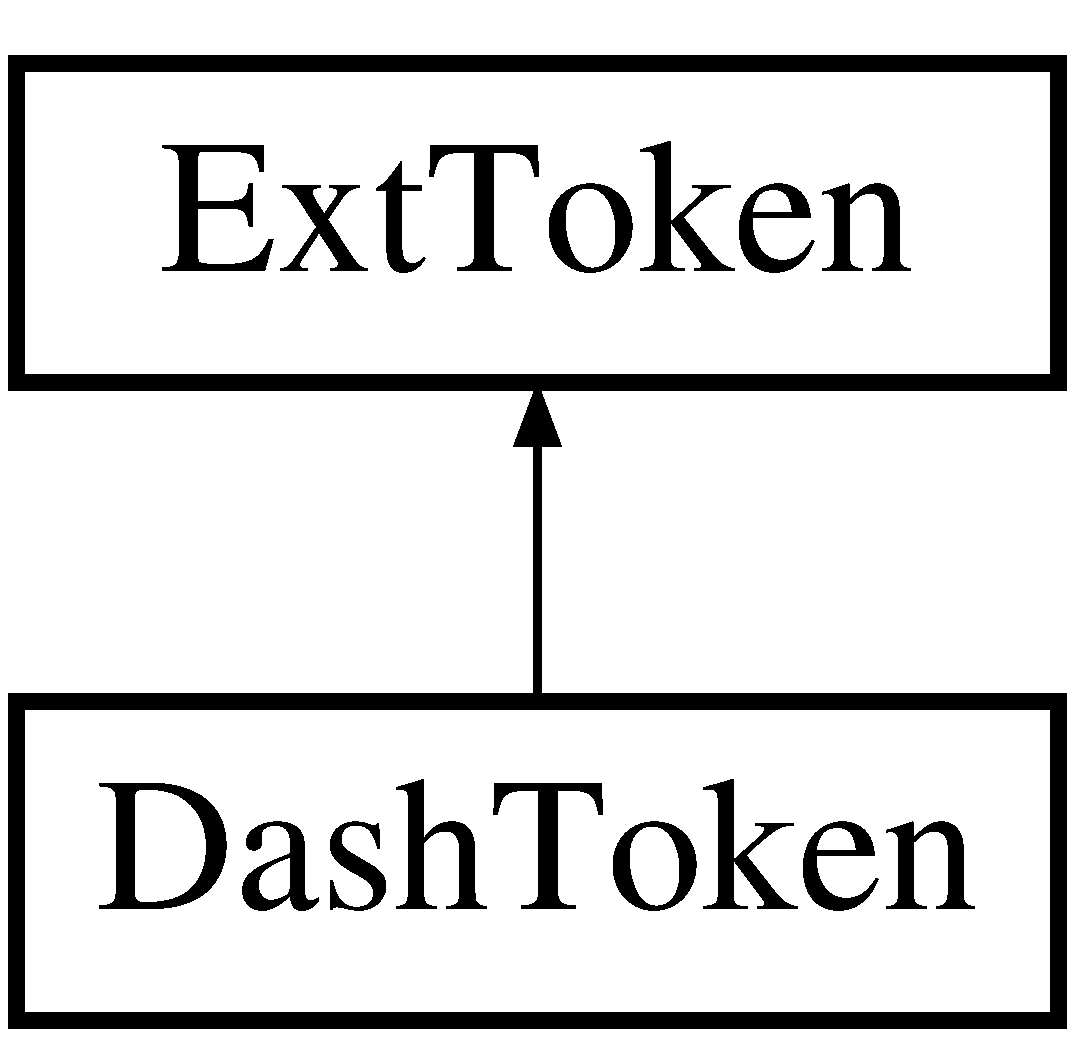
\includegraphics[height=2.000000cm]{classDashToken}
\end{center}
\end{figure}
\subsection*{Public Member Functions}
\begin{DoxyCompactItemize}
\item 
\hypertarget{classDashToken_a9570d66563405c728e679b63a44e53e2}{{\bfseries Dash\-Token} (\hyperlink{classParser}{Parser} $\ast$p, \hyperlink{classToken}{Token} $\ast$t)}\label{classDashToken_a9570d66563405c728e679b63a44e53e2}

\item 
\hypertarget{classDashToken_a703ca6afcd05ac4688c66b82e177bdbc}{\hyperlink{classParseResult}{Parse\-Result} {\bfseries led} (\hyperlink{classParseResult}{Parse\-Result} left)}\label{classDashToken_a703ca6afcd05ac4688c66b82e177bdbc}

\item 
\hypertarget{classDashToken_a02d79abb30dcab20081edb8e969885d2}{std\-::string {\bfseries description} ()}\label{classDashToken_a02d79abb30dcab20081edb8e969885d2}

\item 
\hypertarget{classDashToken_a1cf877584a85c06e884a182744e92b39}{int {\bfseries lbp} ()}\label{classDashToken_a1cf877584a85c06e884a182744e92b39}

\end{DoxyCompactItemize}
\subsection*{Additional Inherited Members}


The documentation for this class was generated from the following file\-:\begin{DoxyCompactItemize}
\item 
ext\-Token.\-h\end{DoxyCompactItemize}

\hypertarget{classDecl}{\section{Decl Class Reference}
\label{classDecl}\index{Decl@{Decl}}
}
Inheritance diagram for Decl\-:\begin{figure}[H]
\begin{center}
\leavevmode
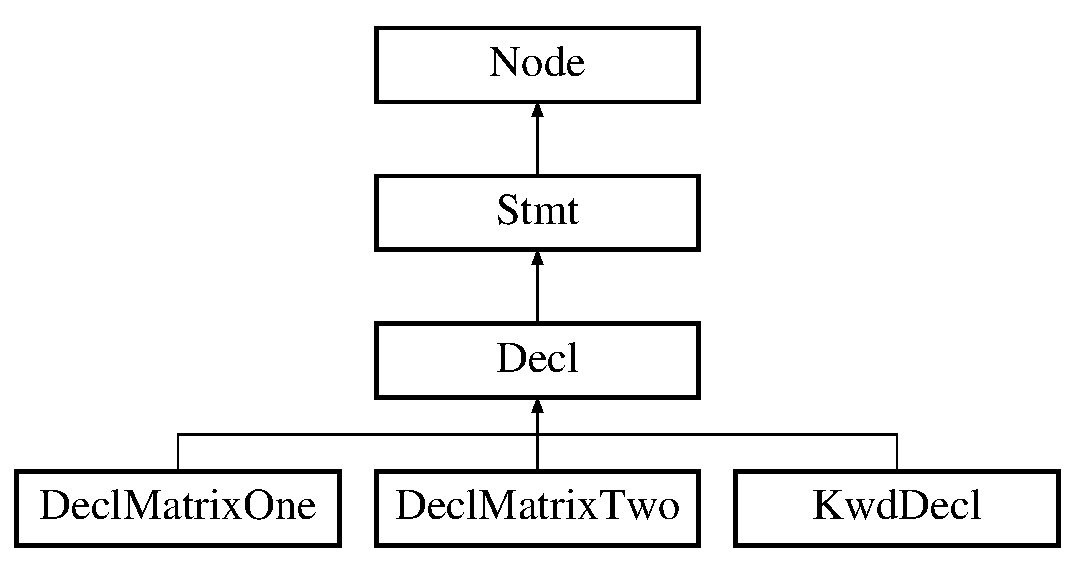
\includegraphics[height=4.000000cm]{classDecl}
\end{center}
\end{figure}
\subsection*{Additional Inherited Members}


The documentation for this class was generated from the following file\-:\begin{DoxyCompactItemize}
\item 
A\-S\-T.\-h\end{DoxyCompactItemize}

\hypertarget{classDeclMatrixOne}{\section{Decl\-Matrix\-One Class Reference}
\label{classDeclMatrixOne}\index{Decl\-Matrix\-One@{Decl\-Matrix\-One}}
}


{\ttfamily \#include $<$A\-S\-T.\-h$>$}

Inheritance diagram for Decl\-Matrix\-One\-:\begin{figure}[H]
\begin{center}
\leavevmode
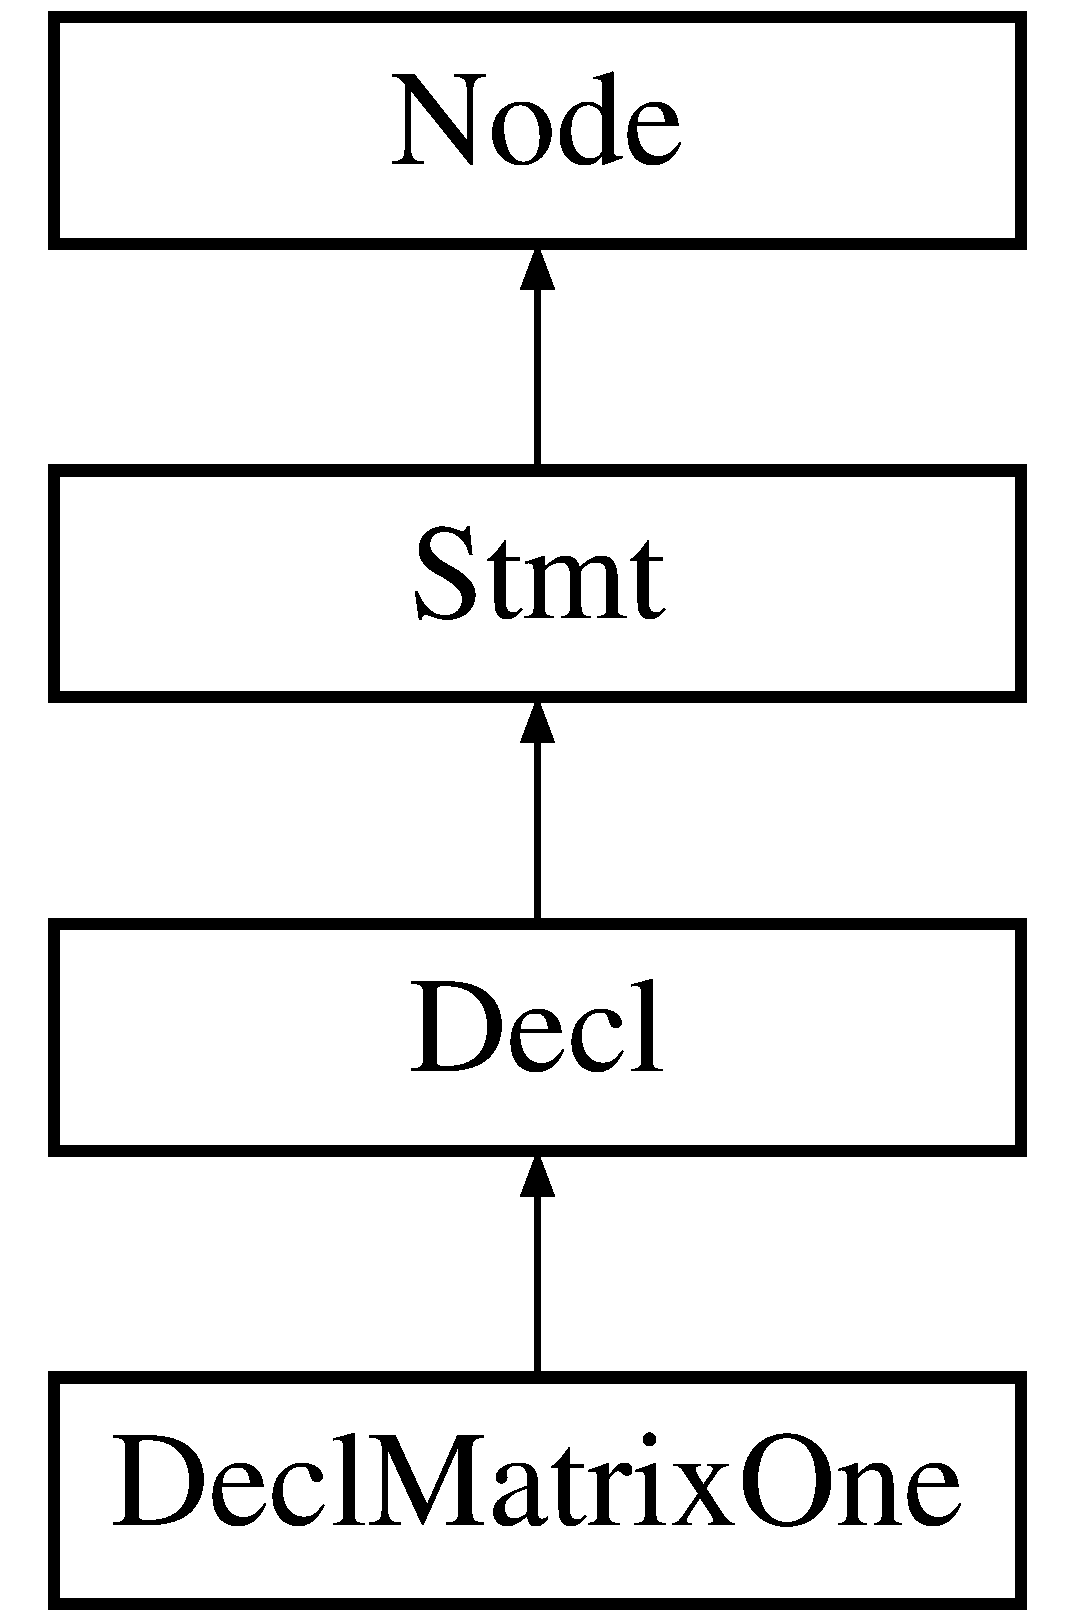
\includegraphics[height=4.000000cm]{classDeclMatrixOne}
\end{center}
\end{figure}
\subsection*{Public Member Functions}
\begin{DoxyCompactItemize}
\item 
\hyperlink{classDeclMatrixOne_aefcbacd4cde0d61d71be293a3ebdff3e}{Decl\-Matrix\-One} (\hyperlink{classVarname}{Varname} $\ast$\-\_\-v, \hyperlink{classExpr}{Expr} $\ast$\-\_\-e, \hyperlink{classExpr}{Expr} $\ast$\-\_\-ee, \hyperlink{classVarname}{Varname} $\ast$\-\_\-vv, \hyperlink{classVarname}{Varname} $\ast$\-\_\-vvv, \hyperlink{classExpr}{Expr} $\ast$\-\_\-eee)
\item 
\hypertarget{classDeclMatrixOne_a4f1a82118dae53dc118cfedb0958c3b5}{std\-::string {\bfseries unparse} ()}\label{classDeclMatrixOne_a4f1a82118dae53dc118cfedb0958c3b5}

\end{DoxyCompactItemize}


\subsection{Detailed Description}
The following two classes is the implementation of matrix declaration, we see two different uses of it here 

\subsection{Constructor \& Destructor Documentation}
\hypertarget{classDeclMatrixOne_aefcbacd4cde0d61d71be293a3ebdff3e}{\index{Decl\-Matrix\-One@{Decl\-Matrix\-One}!Decl\-Matrix\-One@{Decl\-Matrix\-One}}
\index{Decl\-Matrix\-One@{Decl\-Matrix\-One}!DeclMatrixOne@{Decl\-Matrix\-One}}
\subsubsection[{Decl\-Matrix\-One}]{\setlength{\rightskip}{0pt plus 5cm}Decl\-Matrix\-One\-::\-Decl\-Matrix\-One (
\begin{DoxyParamCaption}
\item[{{\bf Varname} $\ast$}]{\-\_\-v, }
\item[{{\bf Expr} $\ast$}]{\-\_\-e, }
\item[{{\bf Expr} $\ast$}]{\-\_\-ee, }
\item[{{\bf Varname} $\ast$}]{\-\_\-vv, }
\item[{{\bf Varname} $\ast$}]{\-\_\-vvv, }
\item[{{\bf Expr} $\ast$}]{\-\_\-eee}
\end{DoxyParamCaption}
)\hspace{0.3cm}{\ttfamily [inline]}}}\label{classDeclMatrixOne_aefcbacd4cde0d61d71be293a3ebdff3e}
The Matrix declaration takes in 6 parameters which define an entry in the matrix 
\begin{DoxyParams}{Parameters}
{\em $\ast$\-\_\-v} & the name of the matrix \\
\hline
{\em \hyperlink{classExpr}{Expr}} & $\ast$\-\_\-e an index bound \\
\hline
{\em \hyperlink{classExpr}{Expr}} & $\ast$\-\_\-ee another index bound \\
\hline
{\em \hyperlink{classVarname}{Varname}} & $\ast$\-\_\-vv index \\
\hline
{\em \hyperlink{classVarname}{Varname}} & $\ast$\-\_\-vvv another index \\
\hline
\end{DoxyParams}


The documentation for this class was generated from the following file\-:\begin{DoxyCompactItemize}
\item 
A\-S\-T.\-h\end{DoxyCompactItemize}

\hypertarget{classDeclMatrixTwo}{\section{Decl\-Matrix\-Two Class Reference}
\label{classDeclMatrixTwo}\index{Decl\-Matrix\-Two@{Decl\-Matrix\-Two}}
}


{\ttfamily \#include $<$A\-S\-T.\-h$>$}

Inheritance diagram for Decl\-Matrix\-Two\-:\begin{figure}[H]
\begin{center}
\leavevmode
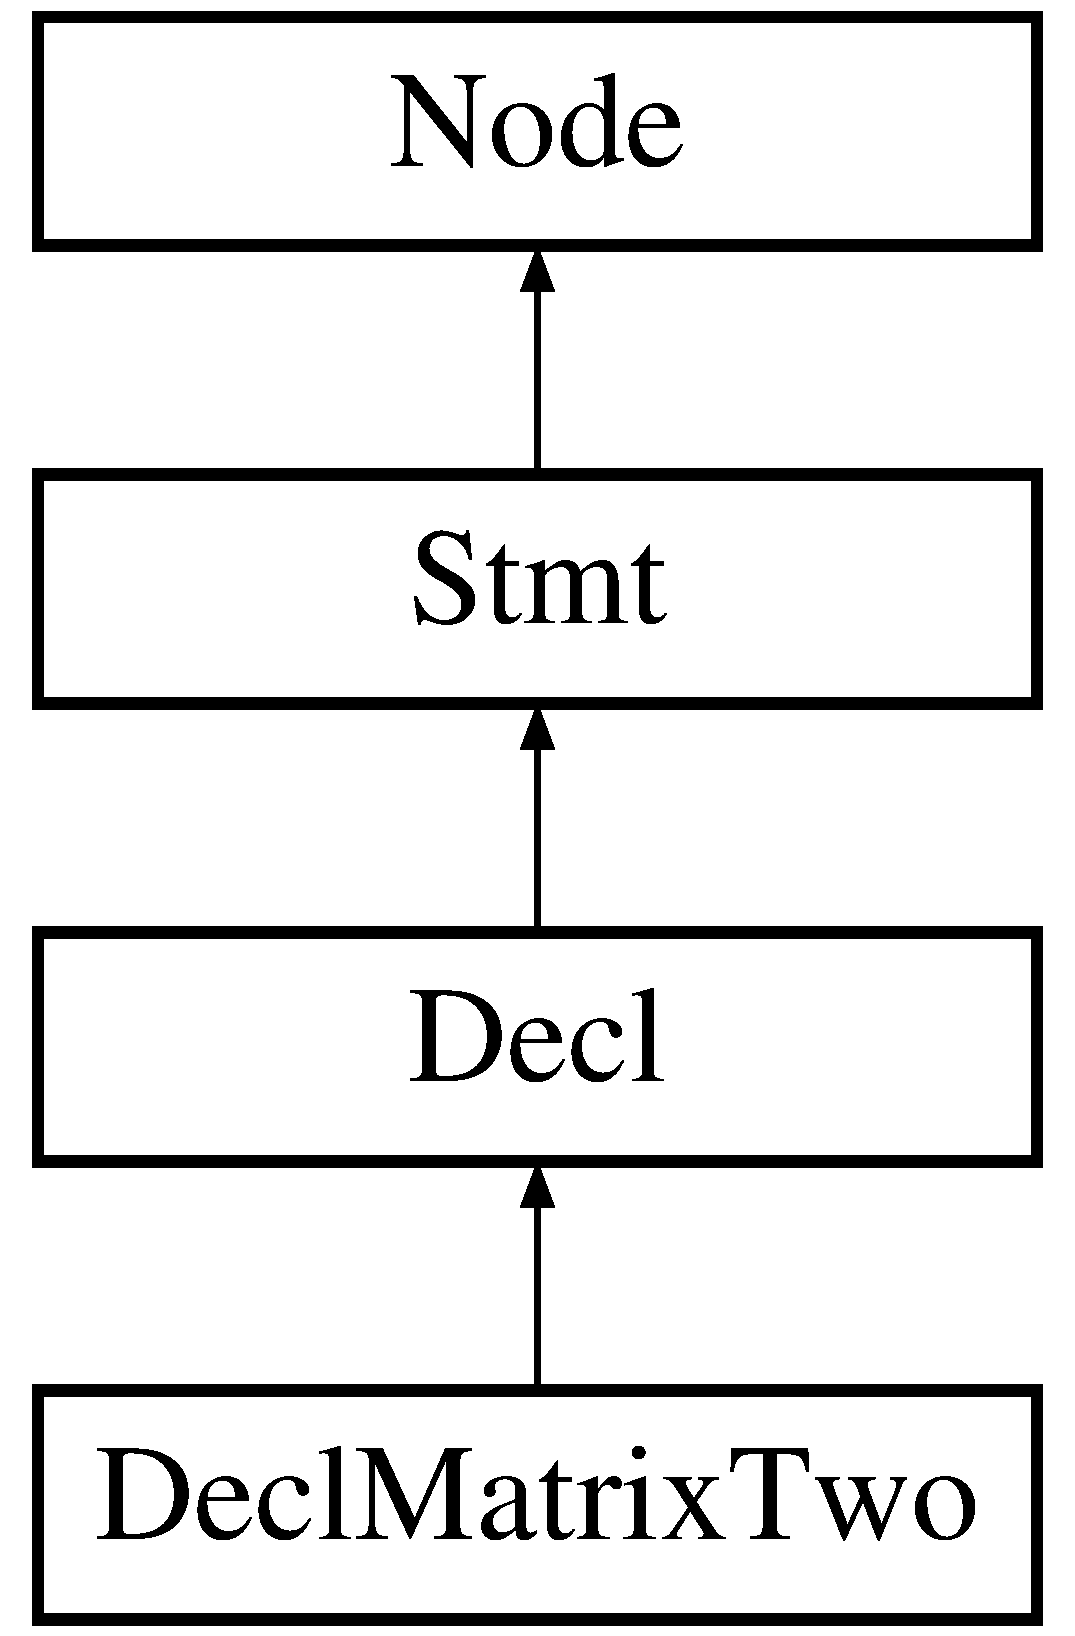
\includegraphics[height=4.000000cm]{classDeclMatrixTwo}
\end{center}
\end{figure}
\subsection*{Public Member Functions}
\begin{DoxyCompactItemize}
\item 
\hypertarget{classDeclMatrixTwo_aef678c4989609d3d780d5c1f71924f0e}{{\bfseries Decl\-Matrix\-Two} (\hyperlink{classVarname}{Varname} $\ast$\-\_\-v, \hyperlink{classExpr}{Expr} $\ast$\-\_\-e)}\label{classDeclMatrixTwo_aef678c4989609d3d780d5c1f71924f0e}

\item 
\hypertarget{classDeclMatrixTwo_af5cb097943bbcb9458704f296d56cc24}{std\-::string {\bfseries unparse} ()}\label{classDeclMatrixTwo_af5cb097943bbcb9458704f296d56cc24}

\end{DoxyCompactItemize}


\subsection{Detailed Description}
Assigns one matrix to another 

The documentation for this class was generated from the following file\-:\begin{DoxyCompactItemize}
\item 
A\-S\-T.\-h\end{DoxyCompactItemize}

\hypertarget{classEmptyStmts}{\section{Empty\-Stmts Class Reference}
\label{classEmptyStmts}\index{Empty\-Stmts@{Empty\-Stmts}}
}


{\ttfamily \#include $<$A\-S\-T.\-h$>$}

Inheritance diagram for Empty\-Stmts\-:\begin{figure}[H]
\begin{center}
\leavevmode
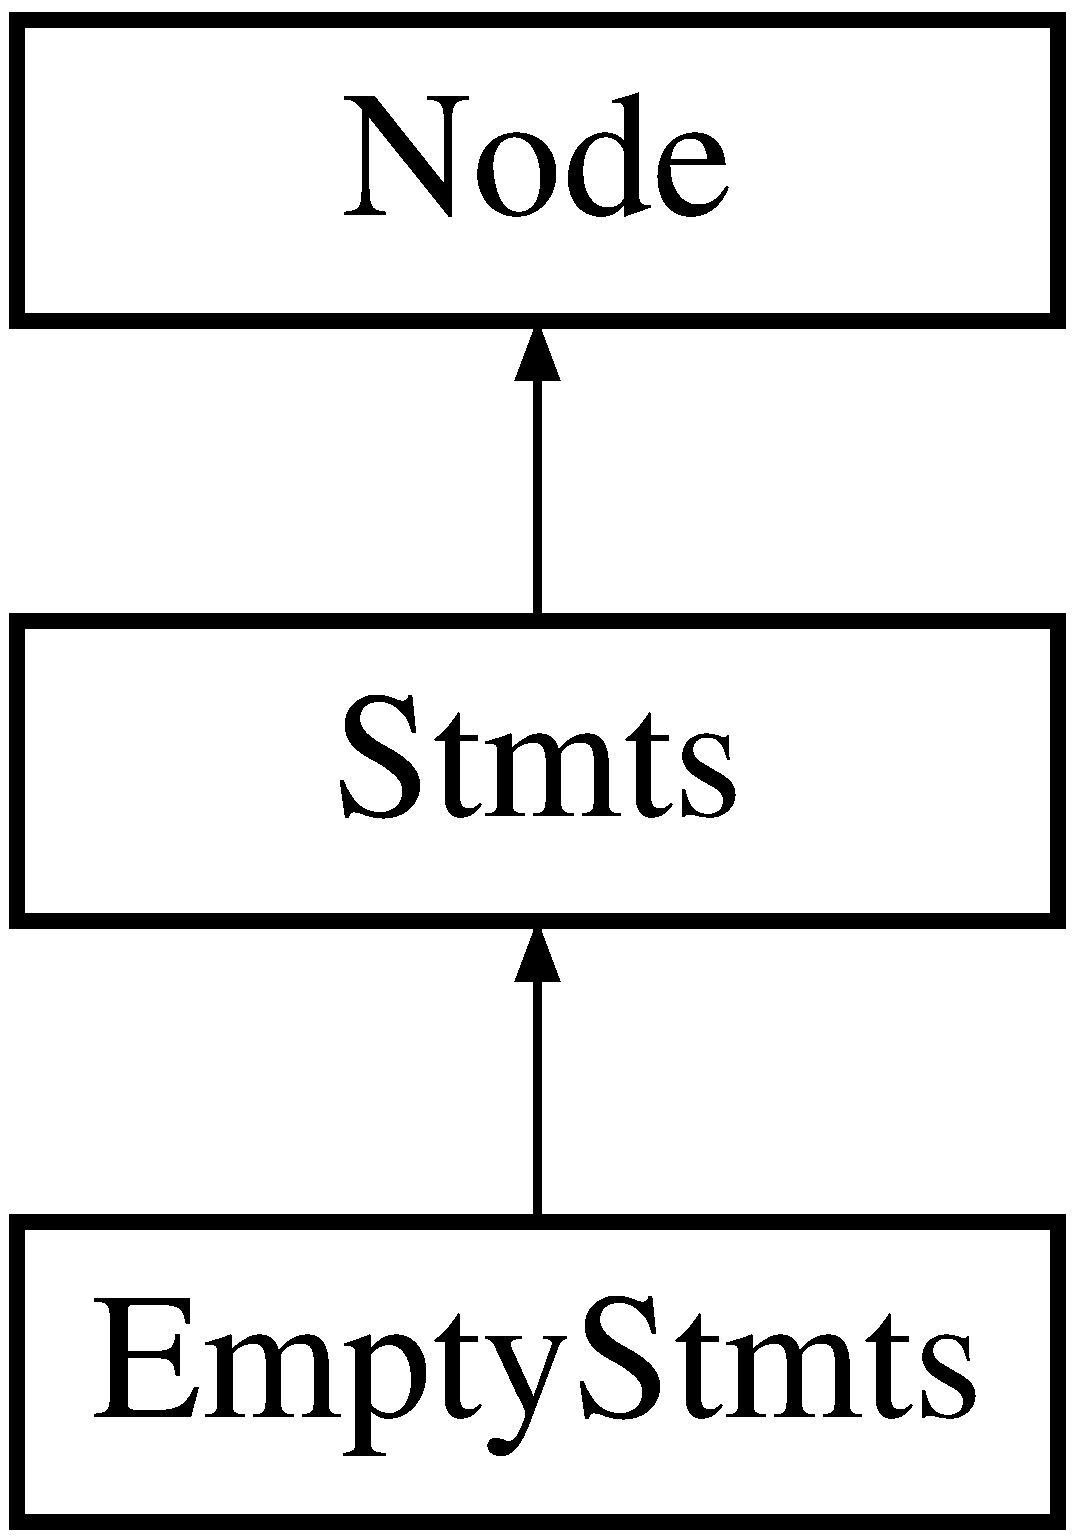
\includegraphics[height=3.000000cm]{classEmptyStmts}
\end{center}
\end{figure}
\subsection*{Public Member Functions}
\begin{DoxyCompactItemize}
\item 
\hypertarget{classEmptyStmts_a127064ef5c59227fc8452b31c65eb905}{std\-::string {\bfseries unparse} ()}\label{classEmptyStmts_a127064ef5c59227fc8452b31c65eb905}

\end{DoxyCompactItemize}


\subsection{Detailed Description}
This class is for empty states for when it reaches the end of the \hyperlink{classStmts}{Stmts} sequence 

The documentation for this class was generated from the following files\-:\begin{DoxyCompactItemize}
\item 
A\-S\-T.\-h\item 
A\-S\-T.\-cpp\end{DoxyCompactItemize}

\hypertarget{classEndOfFileToken}{\section{End\-Of\-File\-Token Class Reference}
\label{classEndOfFileToken}\index{End\-Of\-File\-Token@{End\-Of\-File\-Token}}
}
Inheritance diagram for End\-Of\-File\-Token\-:\begin{figure}[H]
\begin{center}
\leavevmode
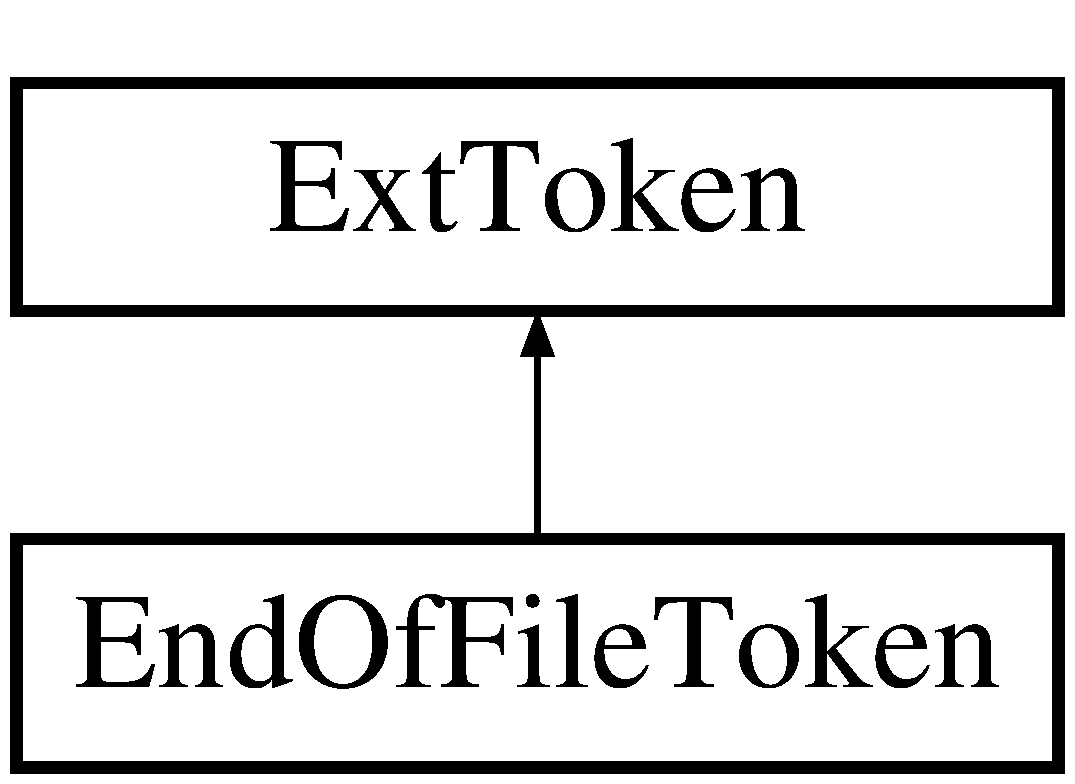
\includegraphics[height=2.000000cm]{classEndOfFileToken}
\end{center}
\end{figure}
\subsection*{Public Member Functions}
\begin{DoxyCompactItemize}
\item 
\hypertarget{classEndOfFileToken_a5c093bc13648a4f4df525ea4242e59d9}{{\bfseries End\-Of\-File\-Token} (\hyperlink{classParser}{Parser} $\ast$p, \hyperlink{classToken}{Token} $\ast$t)}\label{classEndOfFileToken_a5c093bc13648a4f4df525ea4242e59d9}

\item 
\hypertarget{classEndOfFileToken_a918312b101ca8cc7fb5ba4e56bc12b58}{std\-::string {\bfseries description} ()}\label{classEndOfFileToken_a918312b101ca8cc7fb5ba4e56bc12b58}

\end{DoxyCompactItemize}
\subsection*{Additional Inherited Members}


The documentation for this class was generated from the following file\-:\begin{DoxyCompactItemize}
\item 
ext\-Token.\-h\end{DoxyCompactItemize}

\hypertarget{classExpr}{\section{Expr Class Reference}
\label{classExpr}\index{Expr@{Expr}}
}
Inheritance diagram for Expr\-:\begin{figure}[H]
\begin{center}
\leavevmode
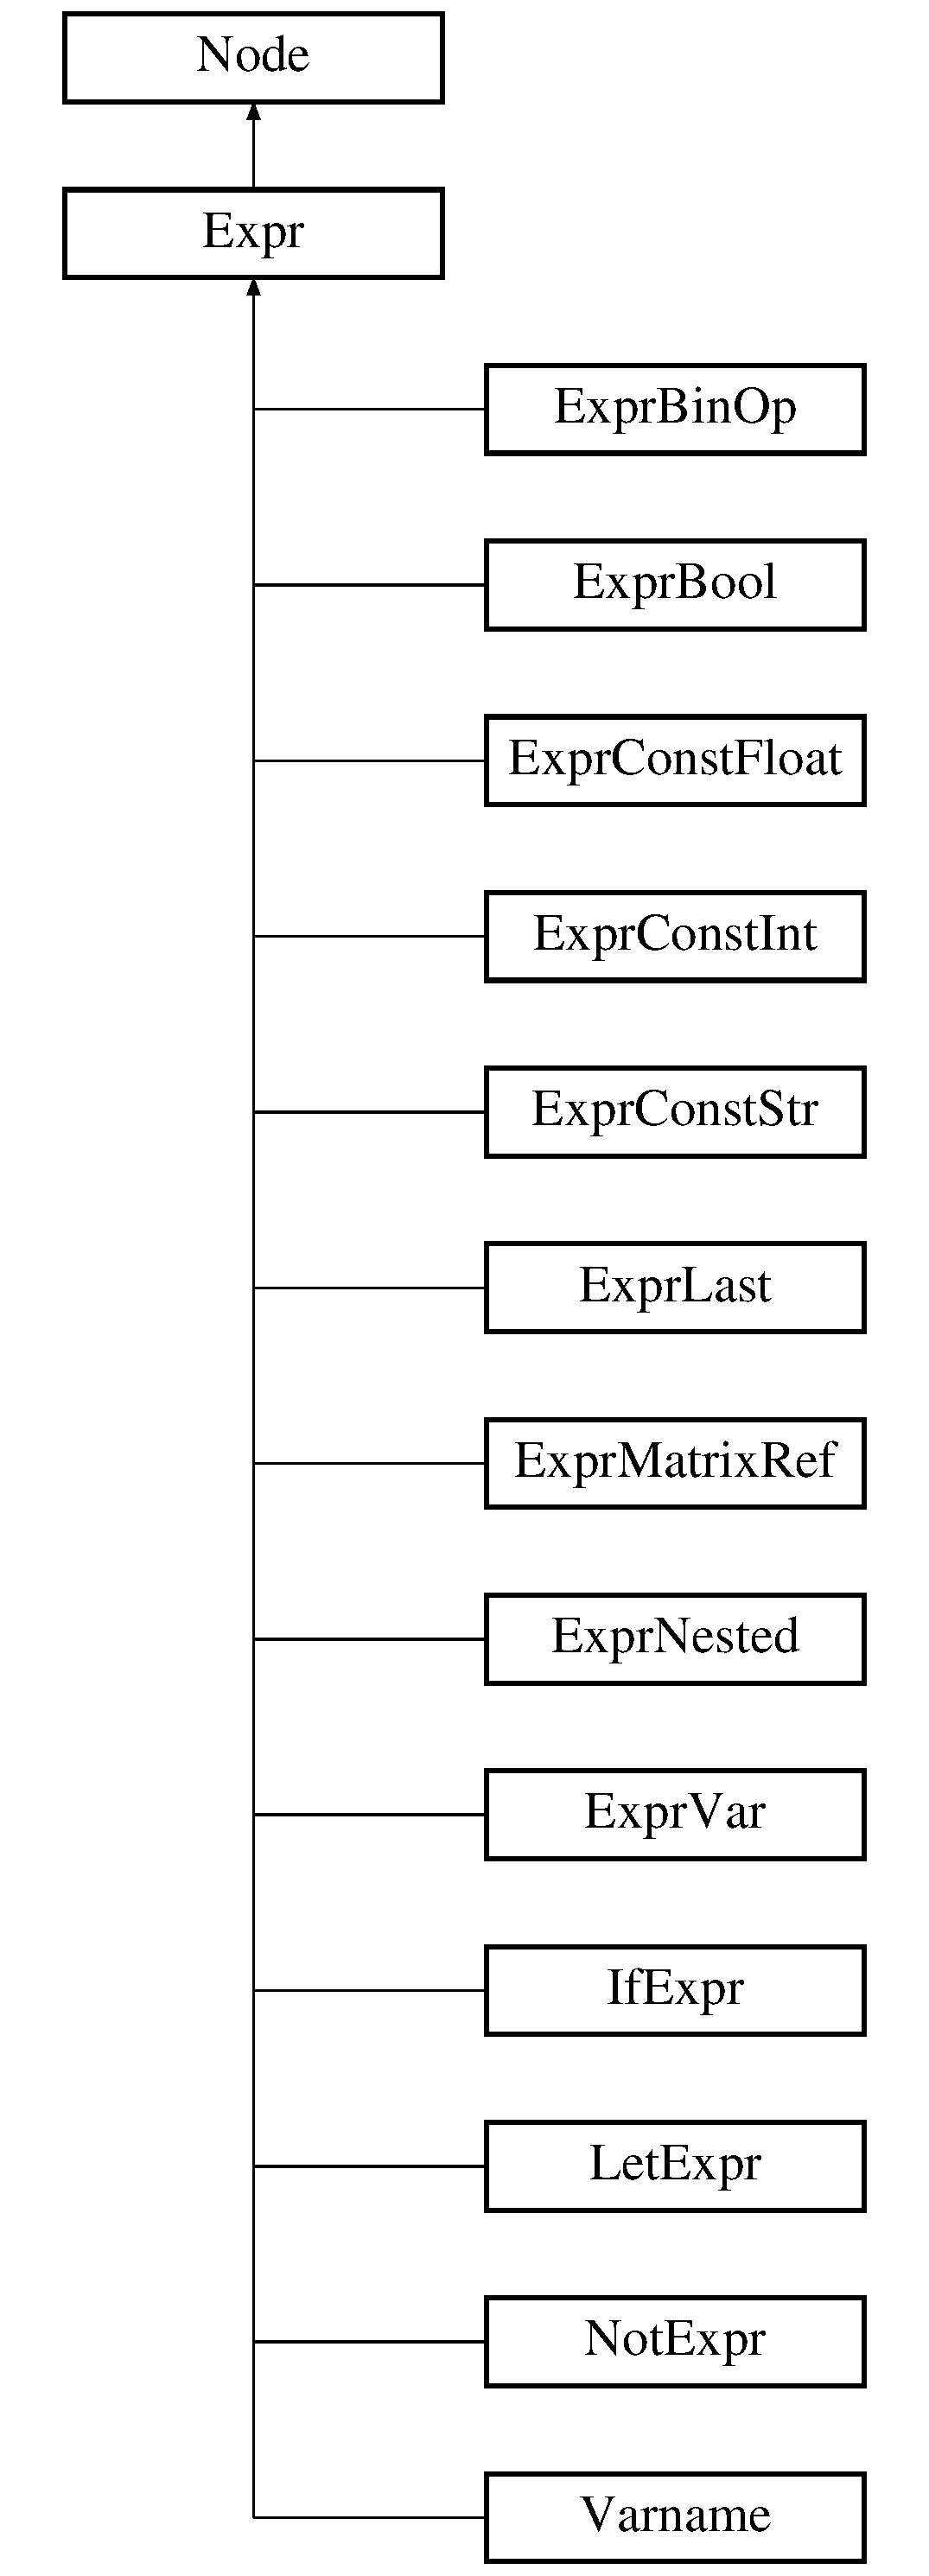
\includegraphics[height=12.000000cm]{classExpr}
\end{center}
\end{figure}
\subsection*{Additional Inherited Members}


The documentation for this class was generated from the following file\-:\begin{DoxyCompactItemize}
\item 
A\-S\-T.\-h\end{DoxyCompactItemize}

\hypertarget{classExprBinOp}{\section{Expr\-Bin\-Op Class Reference}
\label{classExprBinOp}\index{Expr\-Bin\-Op@{Expr\-Bin\-Op}}
}


{\ttfamily \#include $<$A\-S\-T.\-h$>$}

Inheritance diagram for Expr\-Bin\-Op\-:\begin{figure}[H]
\begin{center}
\leavevmode
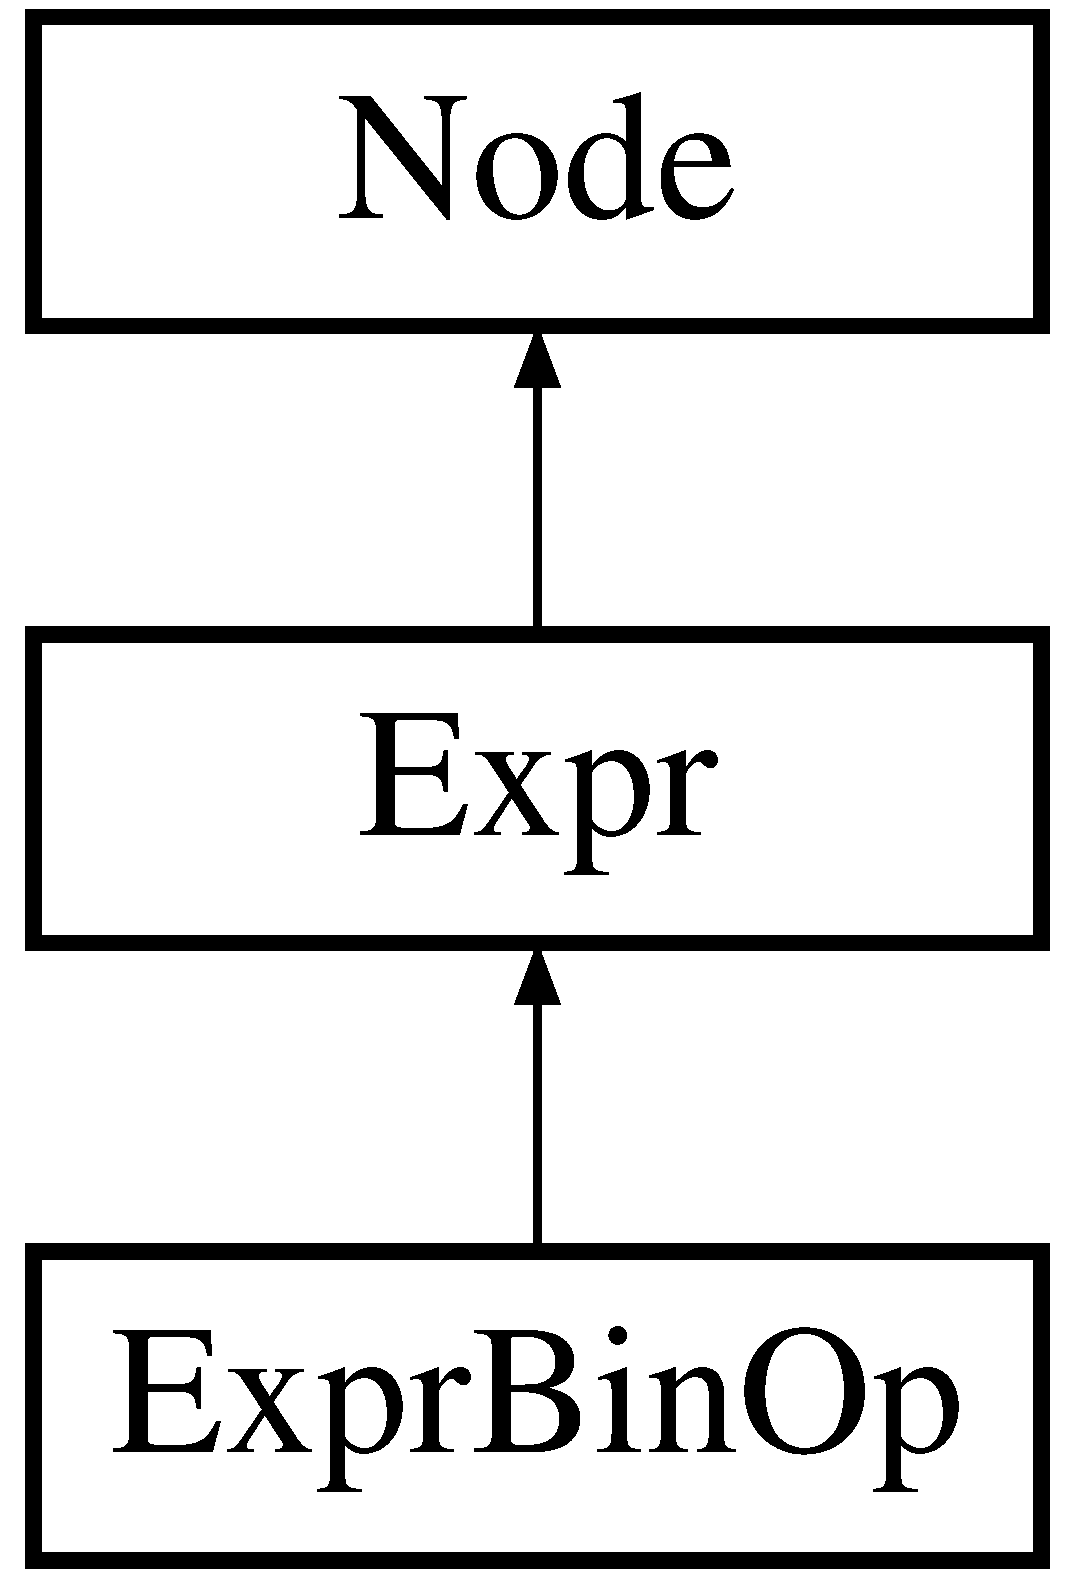
\includegraphics[height=3.000000cm]{classExprBinOp}
\end{center}
\end{figure}
\subsection*{Public Member Functions}
\begin{DoxyCompactItemize}
\item 
\hypertarget{classExprBinOp_a732813d3afa1d4107d50cfa77e8c7f63}{{\bfseries Expr\-Bin\-Op} (\hyperlink{classExpr}{Expr} $\ast$\-\_\-left, std\-::string \-\_\-op, \hyperlink{classExpr}{Expr} $\ast$\-\_\-right)}\label{classExprBinOp_a732813d3afa1d4107d50cfa77e8c7f63}

\item 
\hypertarget{classExprBinOp_a052f921492968fd693186fb92ed28f7b}{std\-::string {\bfseries unparse} ()}\label{classExprBinOp_a052f921492968fd693186fb92ed28f7b}

\end{DoxyCompactItemize}


\subsection{Detailed Description}
This class is for binary operation expressions. These include math operators as well since they all have similar implementation 

The documentation for this class was generated from the following files\-:\begin{DoxyCompactItemize}
\item 
A\-S\-T.\-h\item 
A\-S\-T.\-cpp\end{DoxyCompactItemize}

\hypertarget{classExprBool}{\section{Expr\-Bool Class Reference}
\label{classExprBool}\index{Expr\-Bool@{Expr\-Bool}}
}


{\ttfamily \#include $<$A\-S\-T.\-h$>$}

Inheritance diagram for Expr\-Bool\-:\begin{figure}[H]
\begin{center}
\leavevmode
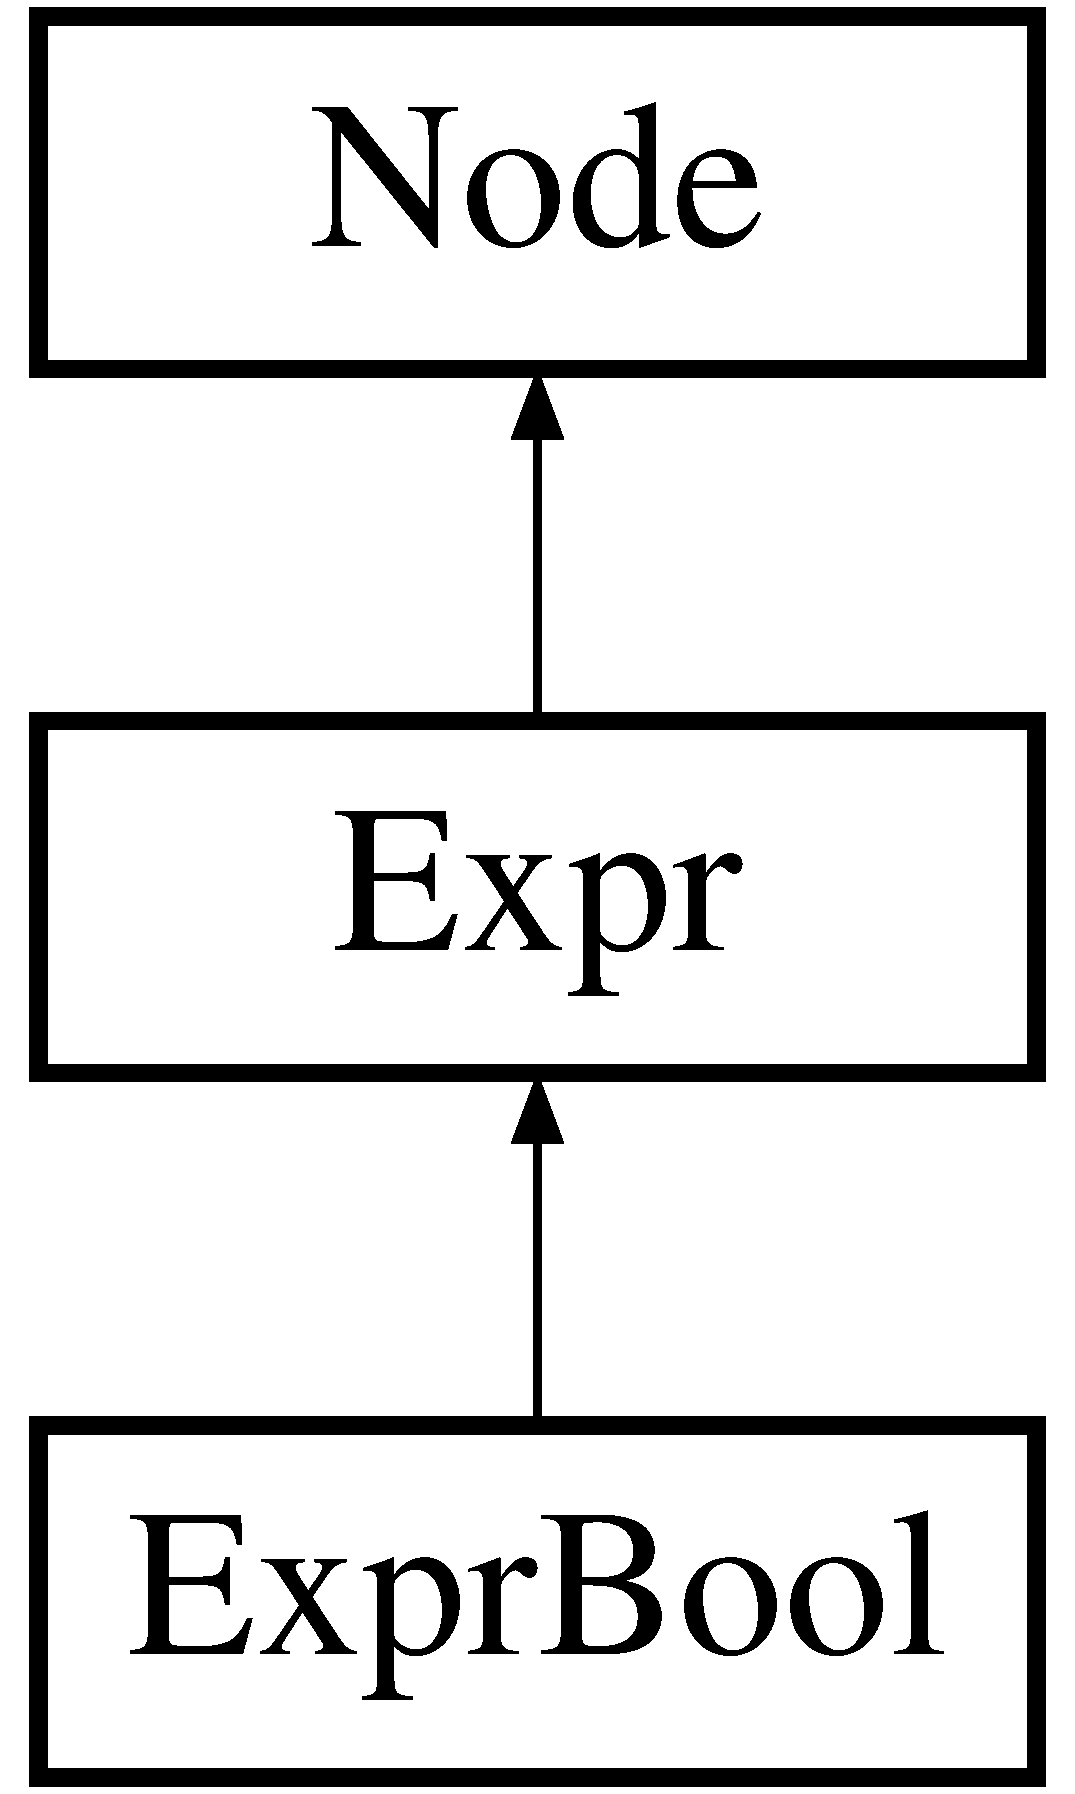
\includegraphics[height=3.000000cm]{classExprBool}
\end{center}
\end{figure}
\subsection*{Public Member Functions}
\begin{DoxyCompactItemize}
\item 
\hypertarget{classExprBool_a4b26eddd21c9659fd94b08fda439956c}{{\bfseries Expr\-Bool} (std\-::string \-\_\-s)}\label{classExprBool_a4b26eddd21c9659fd94b08fda439956c}

\item 
\hypertarget{classExprBool_a925cf97ad93ef6a35cce600ed80f4b5a}{std\-::string {\bfseries unparse} ()}\label{classExprBool_a925cf97ad93ef6a35cce600ed80f4b5a}

\end{DoxyCompactItemize}


\subsection{Detailed Description}
This class is for a boolean expression 

The documentation for this class was generated from the following files\-:\begin{DoxyCompactItemize}
\item 
A\-S\-T.\-h\item 
A\-S\-T.\-cpp\end{DoxyCompactItemize}

\hypertarget{classExprConstFloat}{\section{Expr\-Const\-Float Class Reference}
\label{classExprConstFloat}\index{Expr\-Const\-Float@{Expr\-Const\-Float}}
}
Inheritance diagram for Expr\-Const\-Float\-:\begin{figure}[H]
\begin{center}
\leavevmode
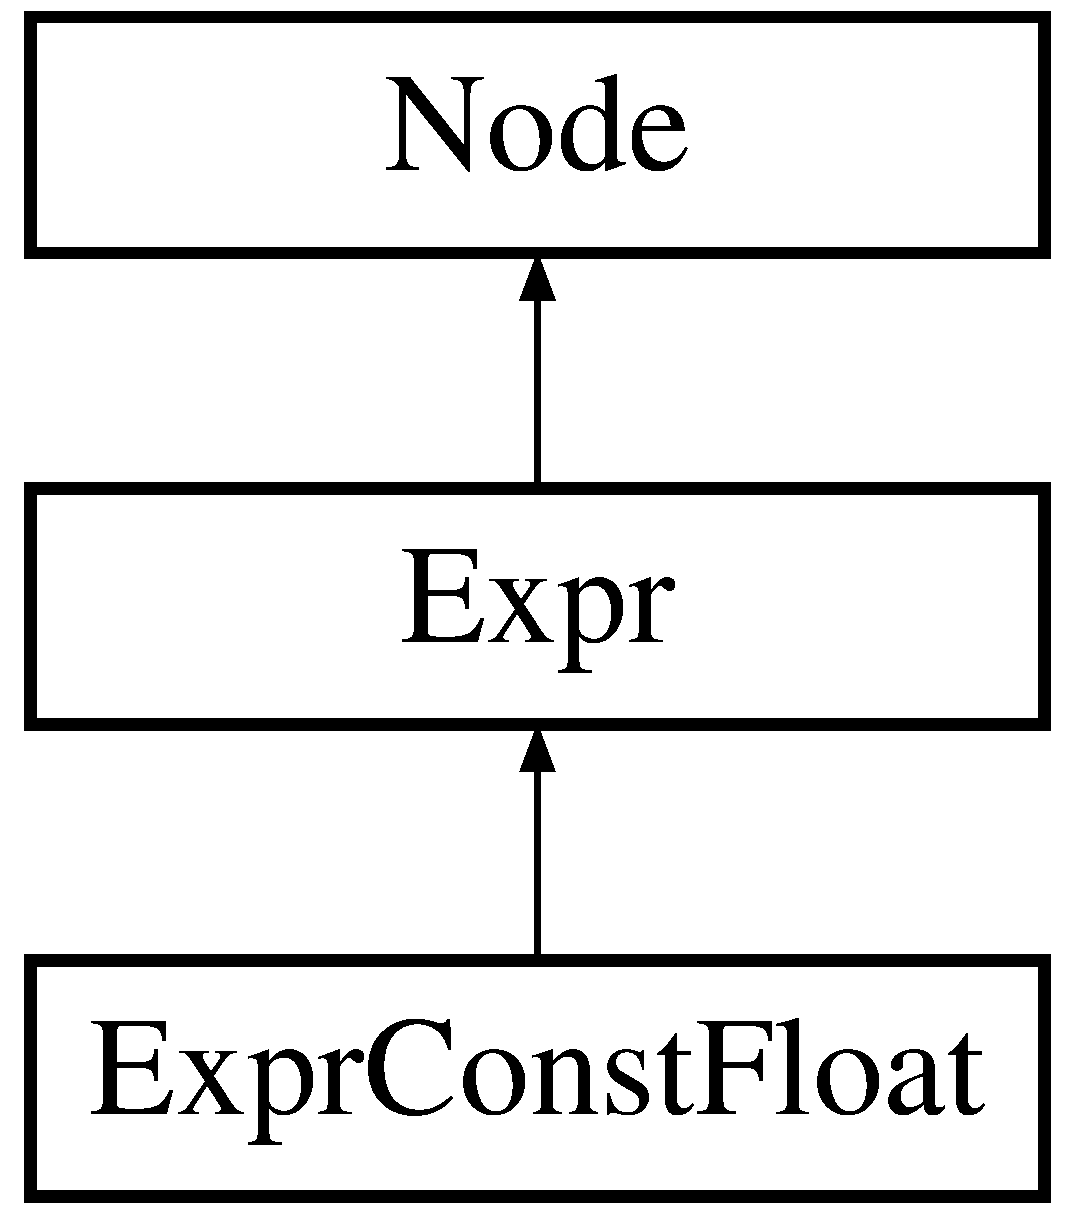
\includegraphics[height=3.000000cm]{classExprConstFloat}
\end{center}
\end{figure}
\subsection*{Public Member Functions}
\begin{DoxyCompactItemize}
\item 
\hypertarget{classExprConstFloat_ae6e4e3f546e3094f5318e834aa12e0f1}{{\bfseries Expr\-Const\-Float} (std\-::string \-\_\-s)}\label{classExprConstFloat_ae6e4e3f546e3094f5318e834aa12e0f1}

\item 
\hypertarget{classExprConstFloat_ab533717ee345d68d7bf4e46fc94572e6}{std\-::string {\bfseries unparse} ()}\label{classExprConstFloat_ab533717ee345d68d7bf4e46fc94572e6}

\end{DoxyCompactItemize}


The documentation for this class was generated from the following files\-:\begin{DoxyCompactItemize}
\item 
A\-S\-T.\-h\item 
A\-S\-T.\-cpp\end{DoxyCompactItemize}

\hypertarget{classExprConstInt}{\section{Expr\-Const\-Int Class Reference}
\label{classExprConstInt}\index{Expr\-Const\-Int@{Expr\-Const\-Int}}
}
Inheritance diagram for Expr\-Const\-Int\-:\begin{figure}[H]
\begin{center}
\leavevmode
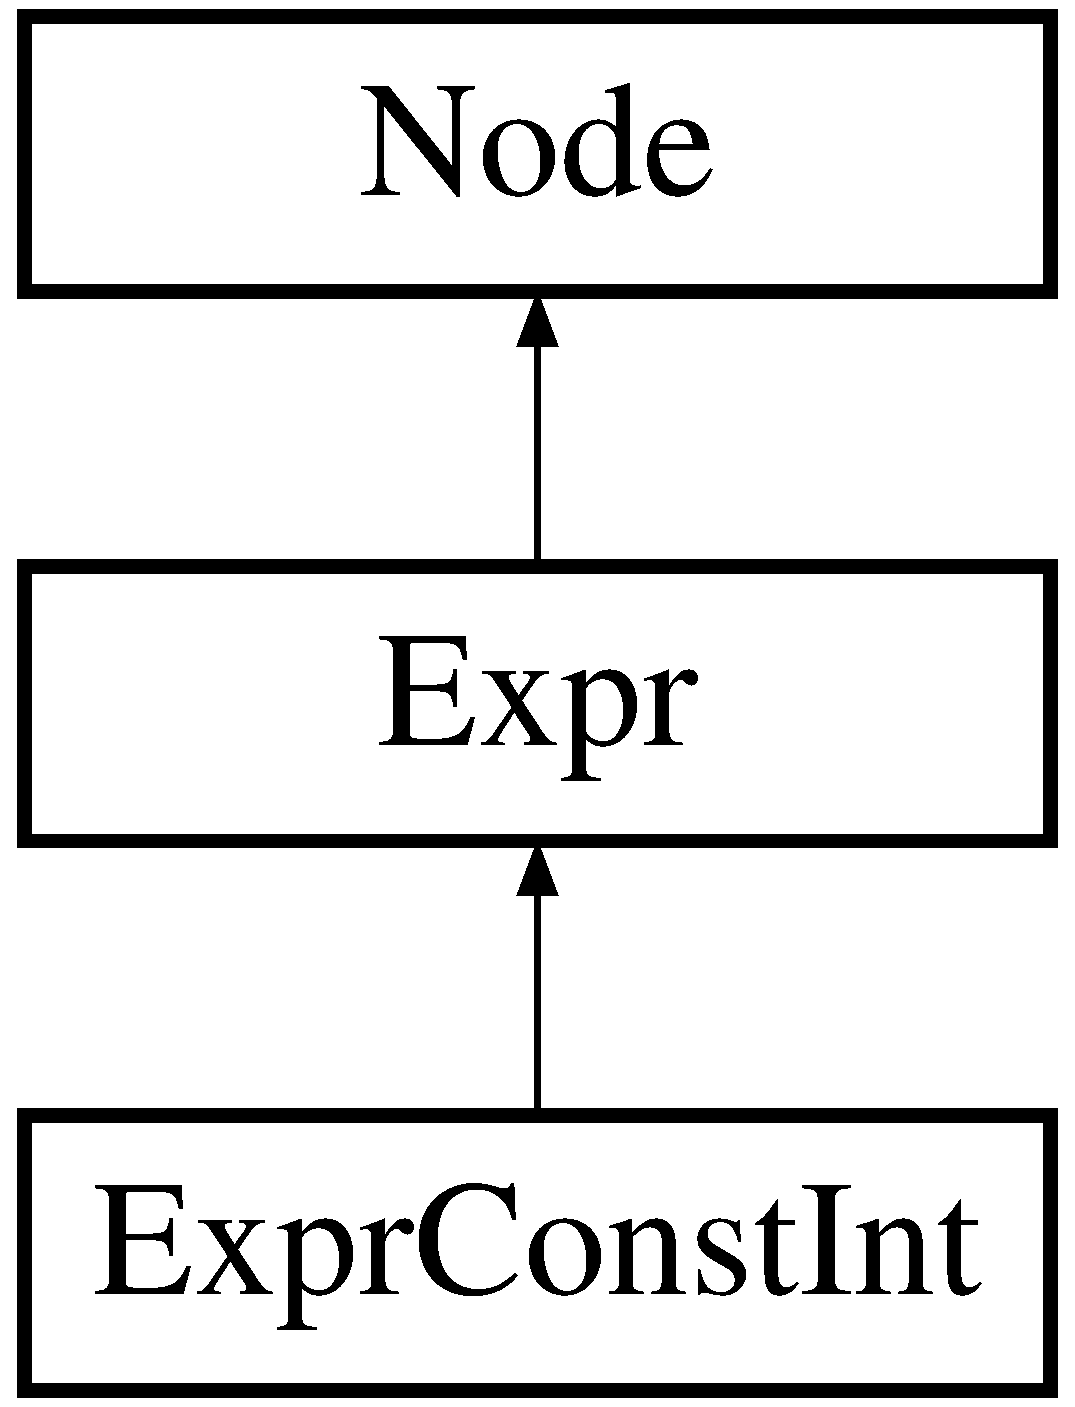
\includegraphics[height=3.000000cm]{classExprConstInt}
\end{center}
\end{figure}
\subsection*{Public Member Functions}
\begin{DoxyCompactItemize}
\item 
\hypertarget{classExprConstInt_aa98ec602e1a565c55926515c77d2d454}{{\bfseries Expr\-Const\-Int} (std\-::string \-\_\-s)}\label{classExprConstInt_aa98ec602e1a565c55926515c77d2d454}

\item 
\hypertarget{classExprConstInt_aa52a073b908704f4924d7fef4ca97a4b}{std\-::string {\bfseries unparse} ()}\label{classExprConstInt_aa52a073b908704f4924d7fef4ca97a4b}

\end{DoxyCompactItemize}


The documentation for this class was generated from the following files\-:\begin{DoxyCompactItemize}
\item 
A\-S\-T.\-h\item 
A\-S\-T.\-cpp\end{DoxyCompactItemize}

\hypertarget{classExprConstStr}{\section{Expr\-Const\-Str Class Reference}
\label{classExprConstStr}\index{Expr\-Const\-Str@{Expr\-Const\-Str}}
}


{\ttfamily \#include $<$A\-S\-T.\-h$>$}

Inheritance diagram for Expr\-Const\-Str\-:\begin{figure}[H]
\begin{center}
\leavevmode
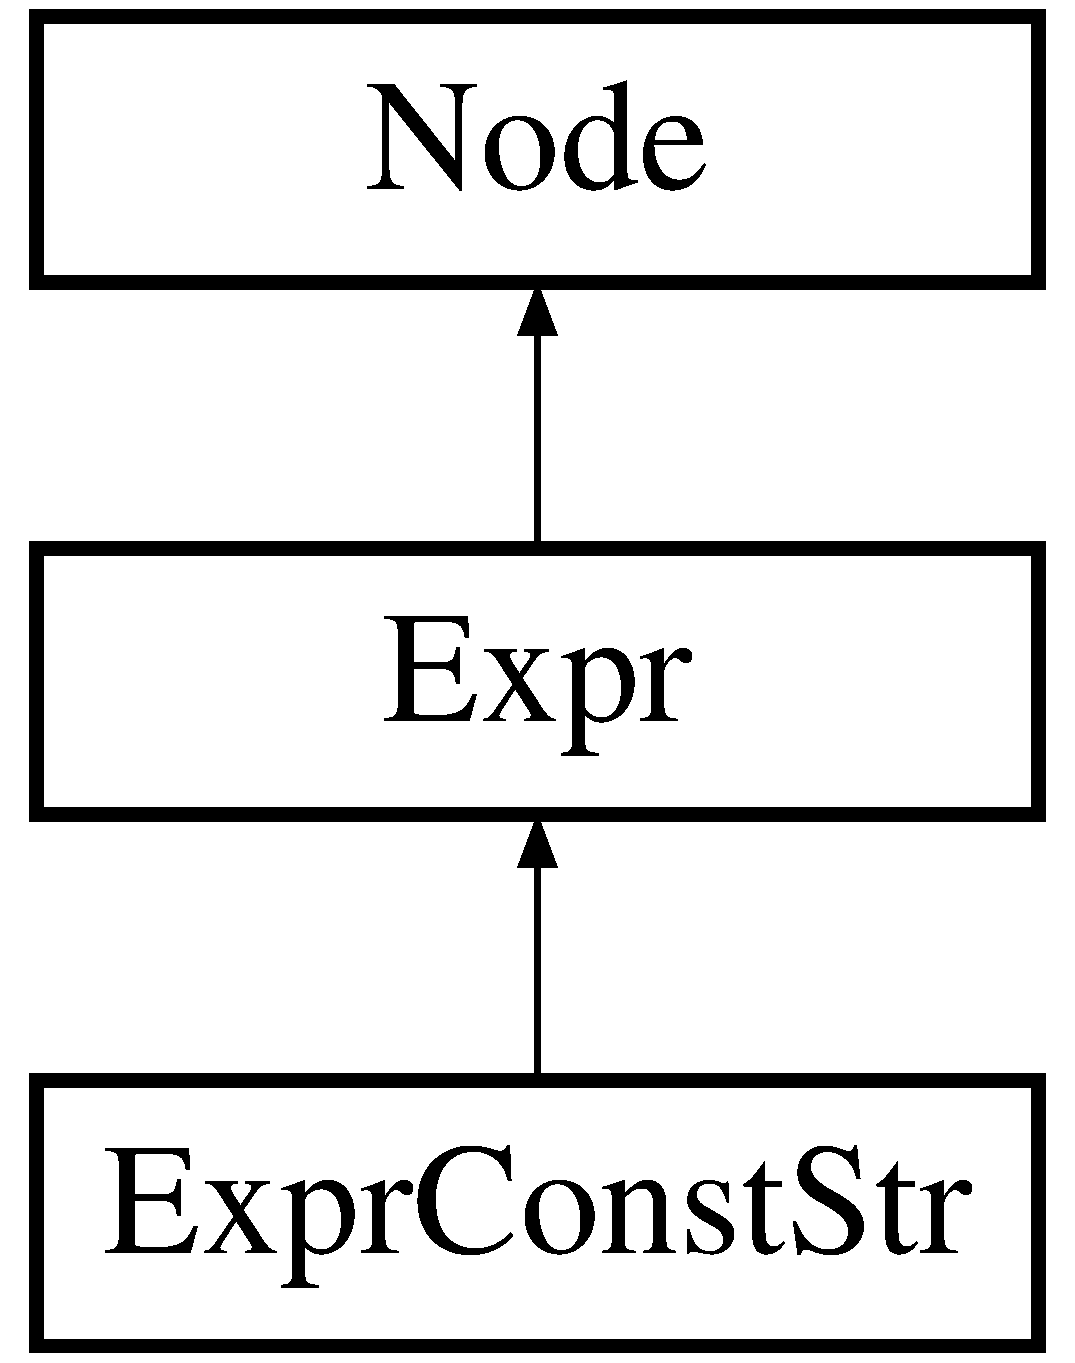
\includegraphics[height=3.000000cm]{classExprConstStr}
\end{center}
\end{figure}
\subsection*{Public Member Functions}
\begin{DoxyCompactItemize}
\item 
\hypertarget{classExprConstStr_af1c65d90e2bccd482f8f0b73b6225f74}{{\bfseries Expr\-Const\-Str} (std\-::string \-\_\-s)}\label{classExprConstStr_af1c65d90e2bccd482f8f0b73b6225f74}

\item 
\hypertarget{classExprConstStr_a13a5a43f7ccdcf01bac1681310d88141}{std\-::string {\bfseries unparse} ()}\label{classExprConstStr_a13a5a43f7ccdcf01bac1681310d88141}

\end{DoxyCompactItemize}


\subsection{Detailed Description}
The following three classes individually store either a integer constant, float constant, or string constant  implemented it like this so that is would be easier implement a value() function on binary op later on 

The documentation for this class was generated from the following files\-:\begin{DoxyCompactItemize}
\item 
A\-S\-T.\-h\item 
A\-S\-T.\-cpp\end{DoxyCompactItemize}

\hypertarget{classExprLast}{\section{Expr\-Last Class Reference}
\label{classExprLast}\index{Expr\-Last@{Expr\-Last}}
}


{\ttfamily \#include $<$A\-S\-T.\-h$>$}

Inheritance diagram for Expr\-Last\-:\begin{figure}[H]
\begin{center}
\leavevmode
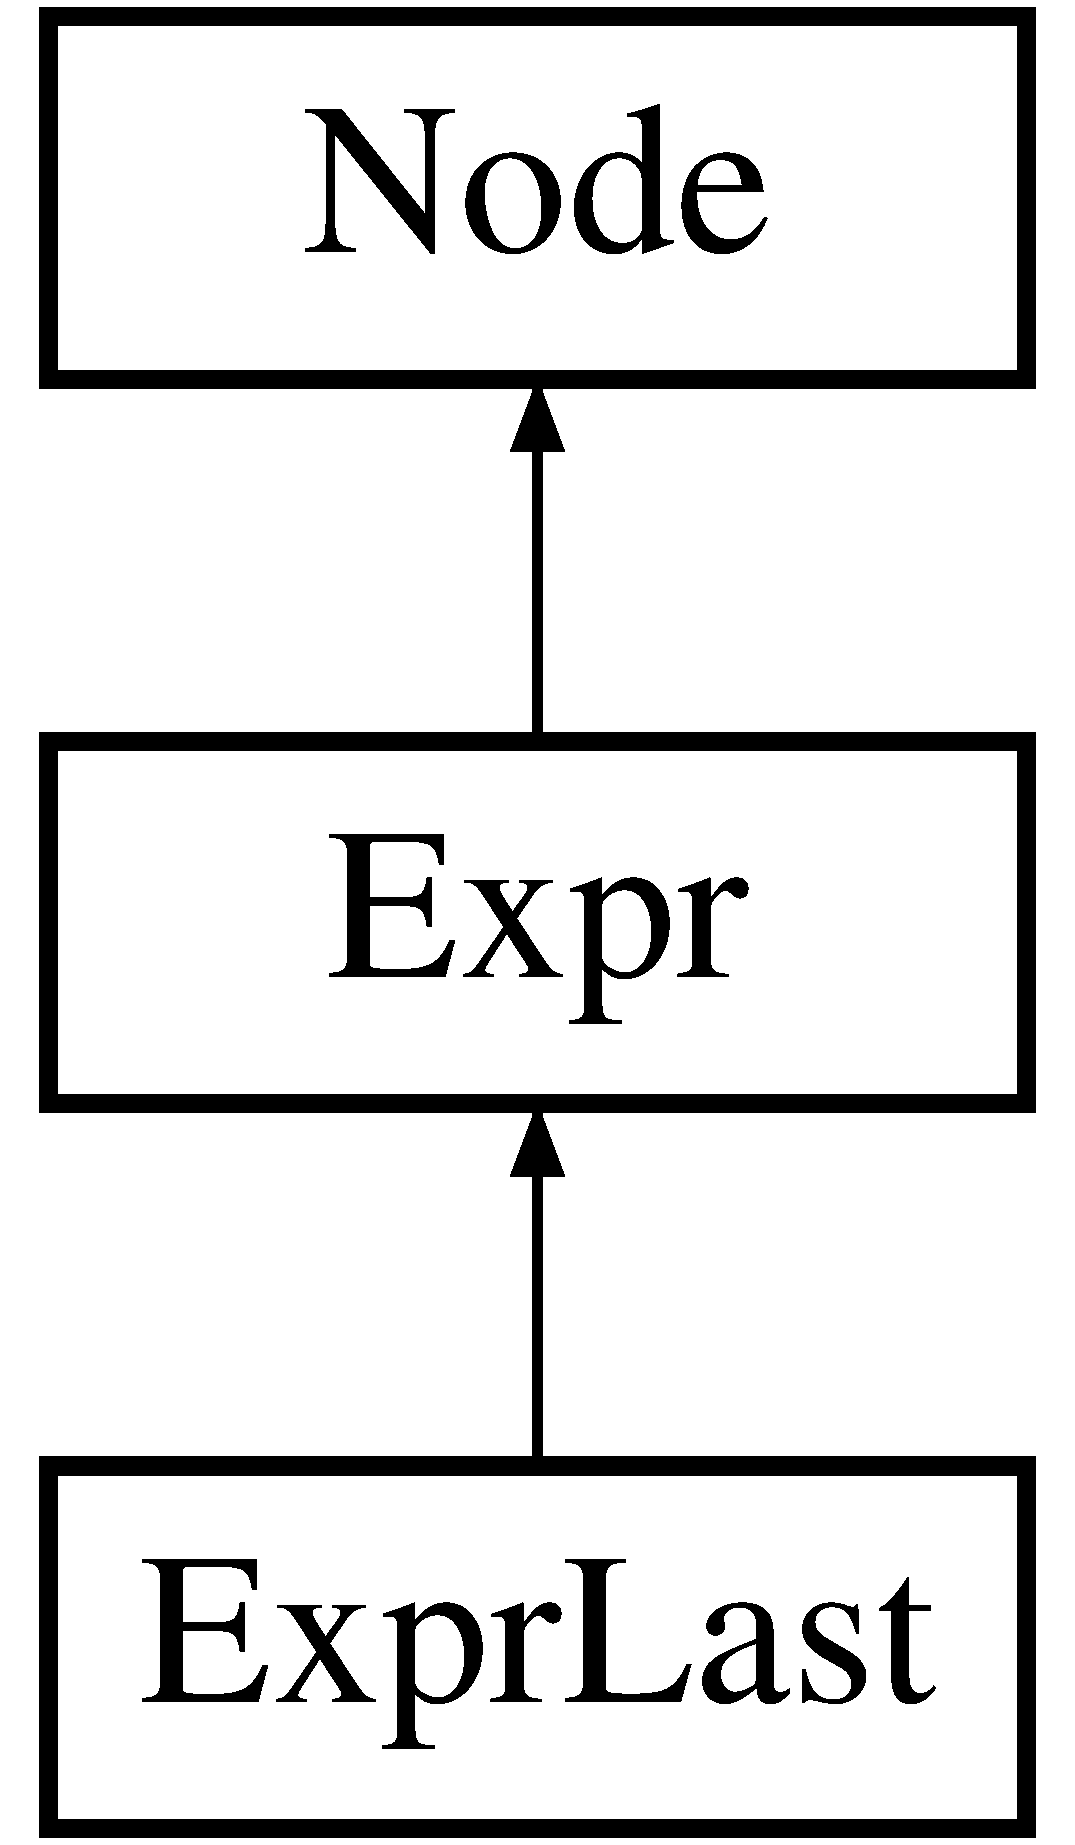
\includegraphics[height=3.000000cm]{classExprLast}
\end{center}
\end{figure}
\subsection*{Public Member Functions}
\begin{DoxyCompactItemize}
\item 
\hypertarget{classExprLast_a361aa1ee38ea15128c7a87f0a2c38925}{{\bfseries Expr\-Last} (\hyperlink{classExpr}{Expr} $\ast$\-\_\-expr)}\label{classExprLast_a361aa1ee38ea15128c7a87f0a2c38925}

\item 
\hypertarget{classExprLast_a038e60a9df13a5d88ee8216b32a70d5c}{std\-::string {\bfseries unparse} ()}\label{classExprLast_a038e60a9df13a5d88ee8216b32a70d5c}

\end{DoxyCompactItemize}


\subsection{Detailed Description}
This if for an expression that is enclosed by parentheses 

The documentation for this class was generated from the following file\-:\begin{DoxyCompactItemize}
\item 
A\-S\-T.\-h\end{DoxyCompactItemize}

\hypertarget{classExprMatrixRef}{\section{Expr\-Matrix\-Ref Class Reference}
\label{classExprMatrixRef}\index{Expr\-Matrix\-Ref@{Expr\-Matrix\-Ref}}
}


{\ttfamily \#include $<$A\-S\-T.\-h$>$}

Inheritance diagram for Expr\-Matrix\-Ref\-:\begin{figure}[H]
\begin{center}
\leavevmode
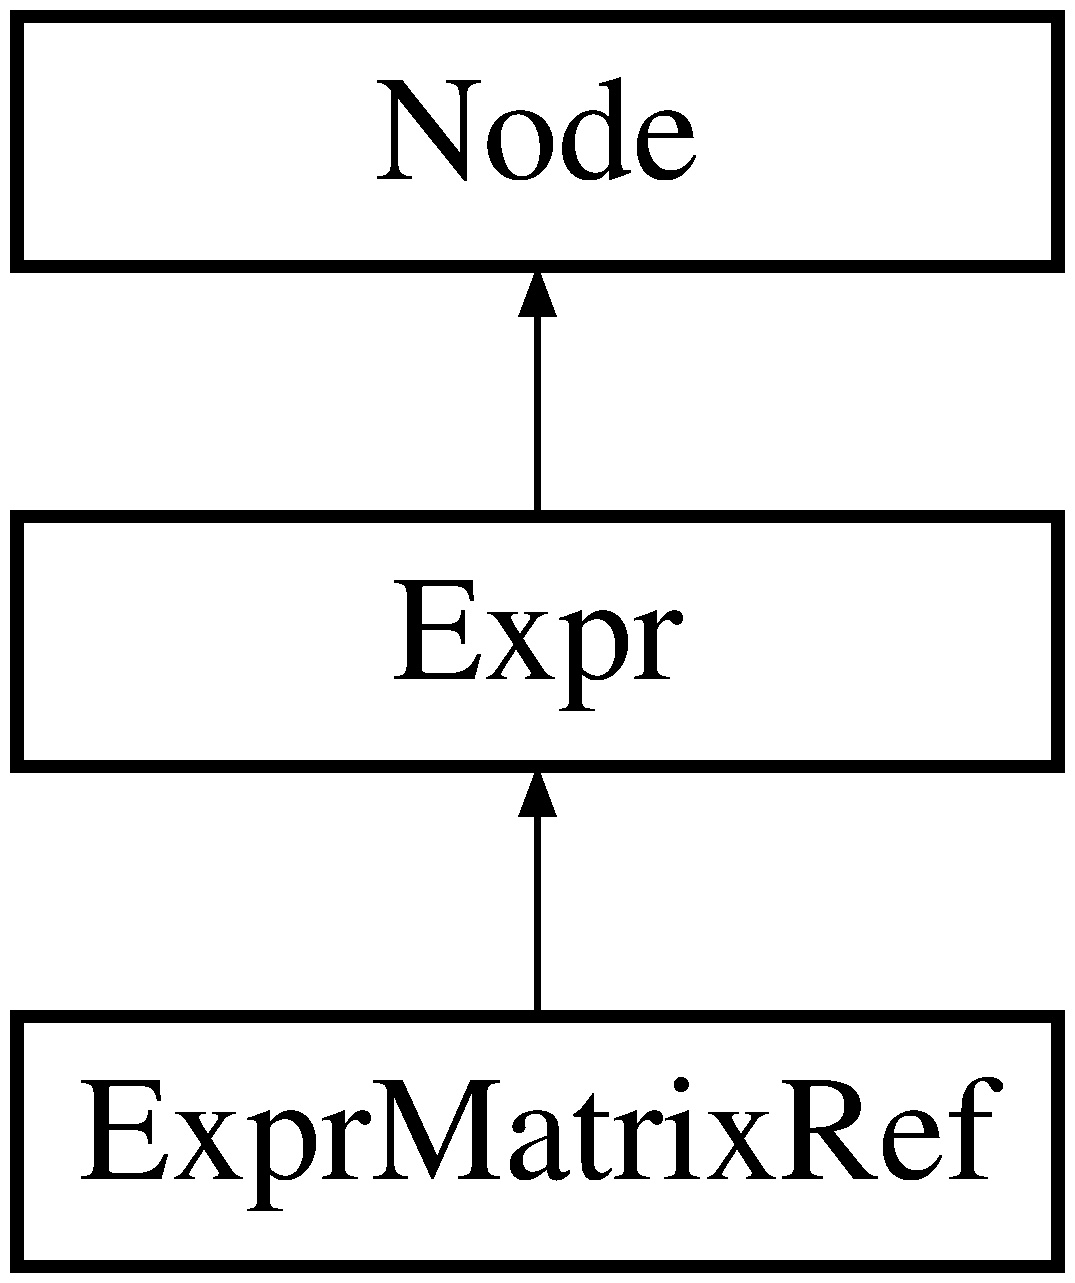
\includegraphics[height=3.000000cm]{classExprMatrixRef}
\end{center}
\end{figure}
\subsection*{Public Member Functions}
\begin{DoxyCompactItemize}
\item 
\hypertarget{classExprMatrixRef_acb47d15f251aa5e6ec01b5b6b8676c20}{{\bfseries Expr\-Matrix\-Ref} (\hyperlink{classVarname}{Varname} $\ast$\-\_\-v, \hyperlink{classExpr}{Expr} $\ast$\-\_\-left, \hyperlink{classExpr}{Expr} $\ast$\-\_\-right)}\label{classExprMatrixRef_acb47d15f251aa5e6ec01b5b6b8676c20}

\item 
\hypertarget{classExprMatrixRef_a44f50ae1ad2b5b69968e3618fca808b9}{std\-::string {\bfseries unparse} ()}\label{classExprMatrixRef_a44f50ae1ad2b5b69968e3618fca808b9}

\end{DoxyCompactItemize}


\subsection{Detailed Description}
This class is similar to the \hyperlink{classVarname}{Varname} in terms of how its used in the grammar, the  point to a single entry in the martix which is itself an expression 

The documentation for this class was generated from the following file\-:\begin{DoxyCompactItemize}
\item 
A\-S\-T.\-h\end{DoxyCompactItemize}

\hypertarget{classExprNested}{\section{Expr\-Nested Class Reference}
\label{classExprNested}\index{Expr\-Nested@{Expr\-Nested}}
}


{\ttfamily \#include $<$A\-S\-T.\-h$>$}

Inheritance diagram for Expr\-Nested\-:\begin{figure}[H]
\begin{center}
\leavevmode
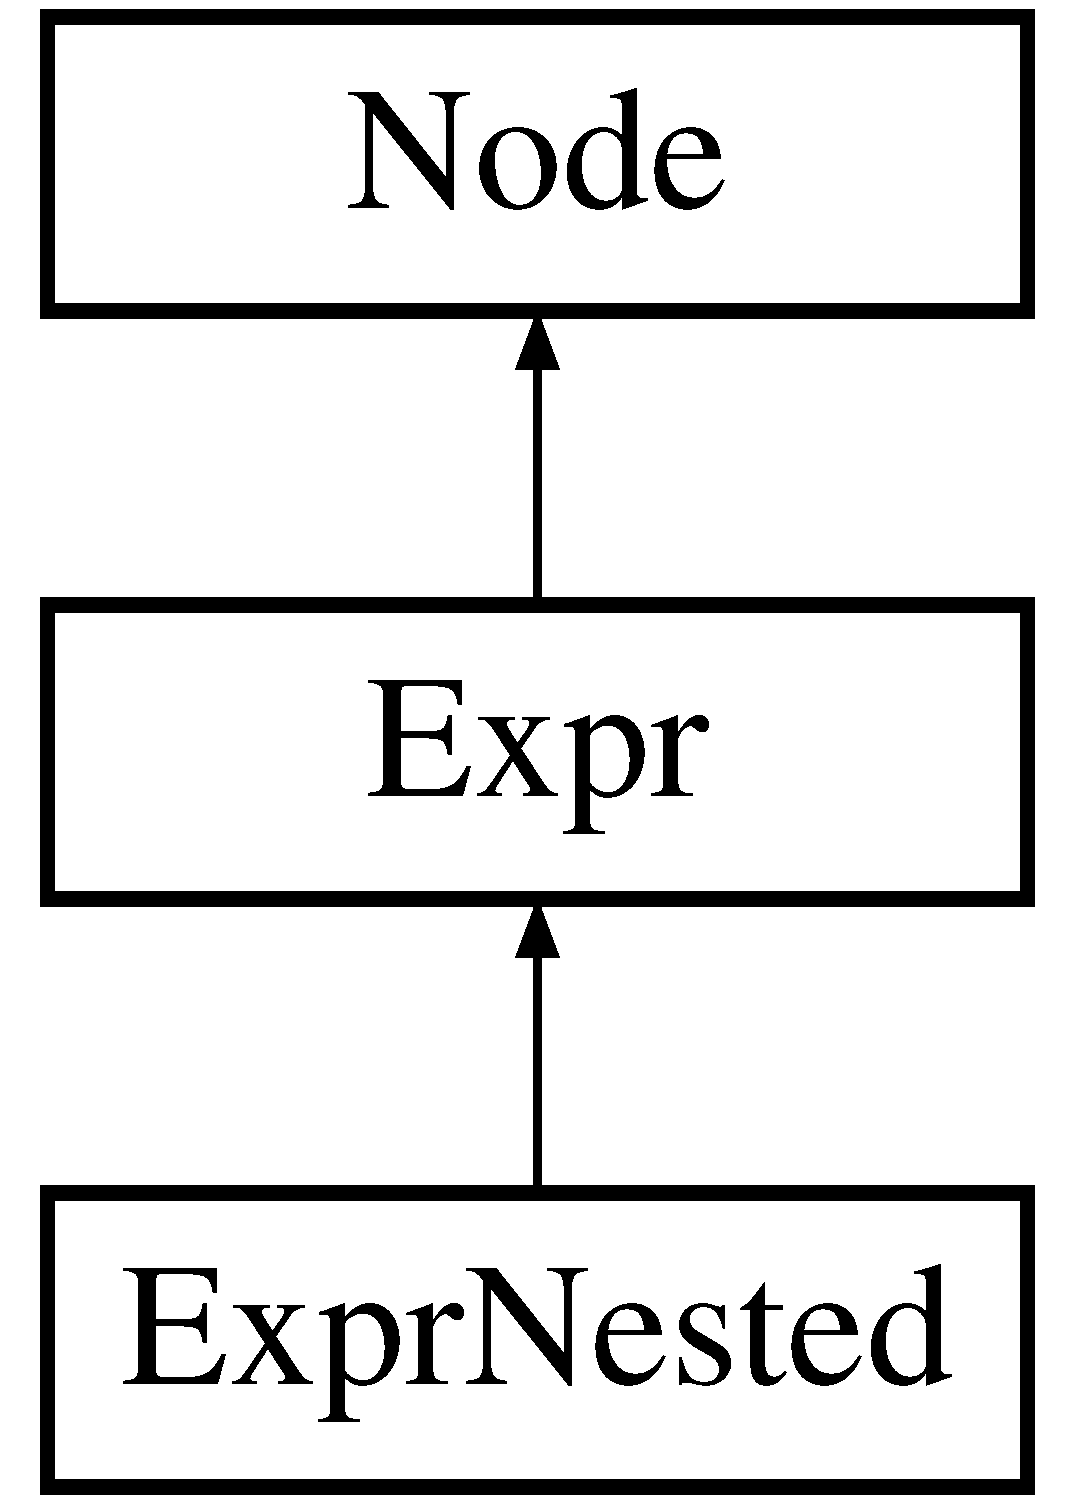
\includegraphics[height=3.000000cm]{classExprNested}
\end{center}
\end{figure}
\subsection*{Public Member Functions}
\begin{DoxyCompactItemize}
\item 
\hypertarget{classExprNested_a0aa61624ac4528977c3d797715f2a710}{{\bfseries Expr\-Nested} (\hyperlink{classVarname}{Varname} $\ast$\-\_\-v, \hyperlink{classExpr}{Expr} $\ast$\-\_\-expr)}\label{classExprNested_a0aa61624ac4528977c3d797715f2a710}

\item 
\hypertarget{classExprNested_ae896b532fe8b1fd25c0e4d4765458d45}{std\-::string {\bfseries unparse} ()}\label{classExprNested_ae896b532fe8b1fd25c0e4d4765458d45}

\end{DoxyCompactItemize}


\subsection{Detailed Description}
This class is for a nested or function call 

The documentation for this class was generated from the following file\-:\begin{DoxyCompactItemize}
\item 
A\-S\-T.\-h\end{DoxyCompactItemize}

\hypertarget{classExprVar}{\section{Expr\-Var Class Reference}
\label{classExprVar}\index{Expr\-Var@{Expr\-Var}}
}


{\ttfamily \#include $<$A\-S\-T.\-h$>$}

Inheritance diagram for Expr\-Var\-:\begin{figure}[H]
\begin{center}
\leavevmode
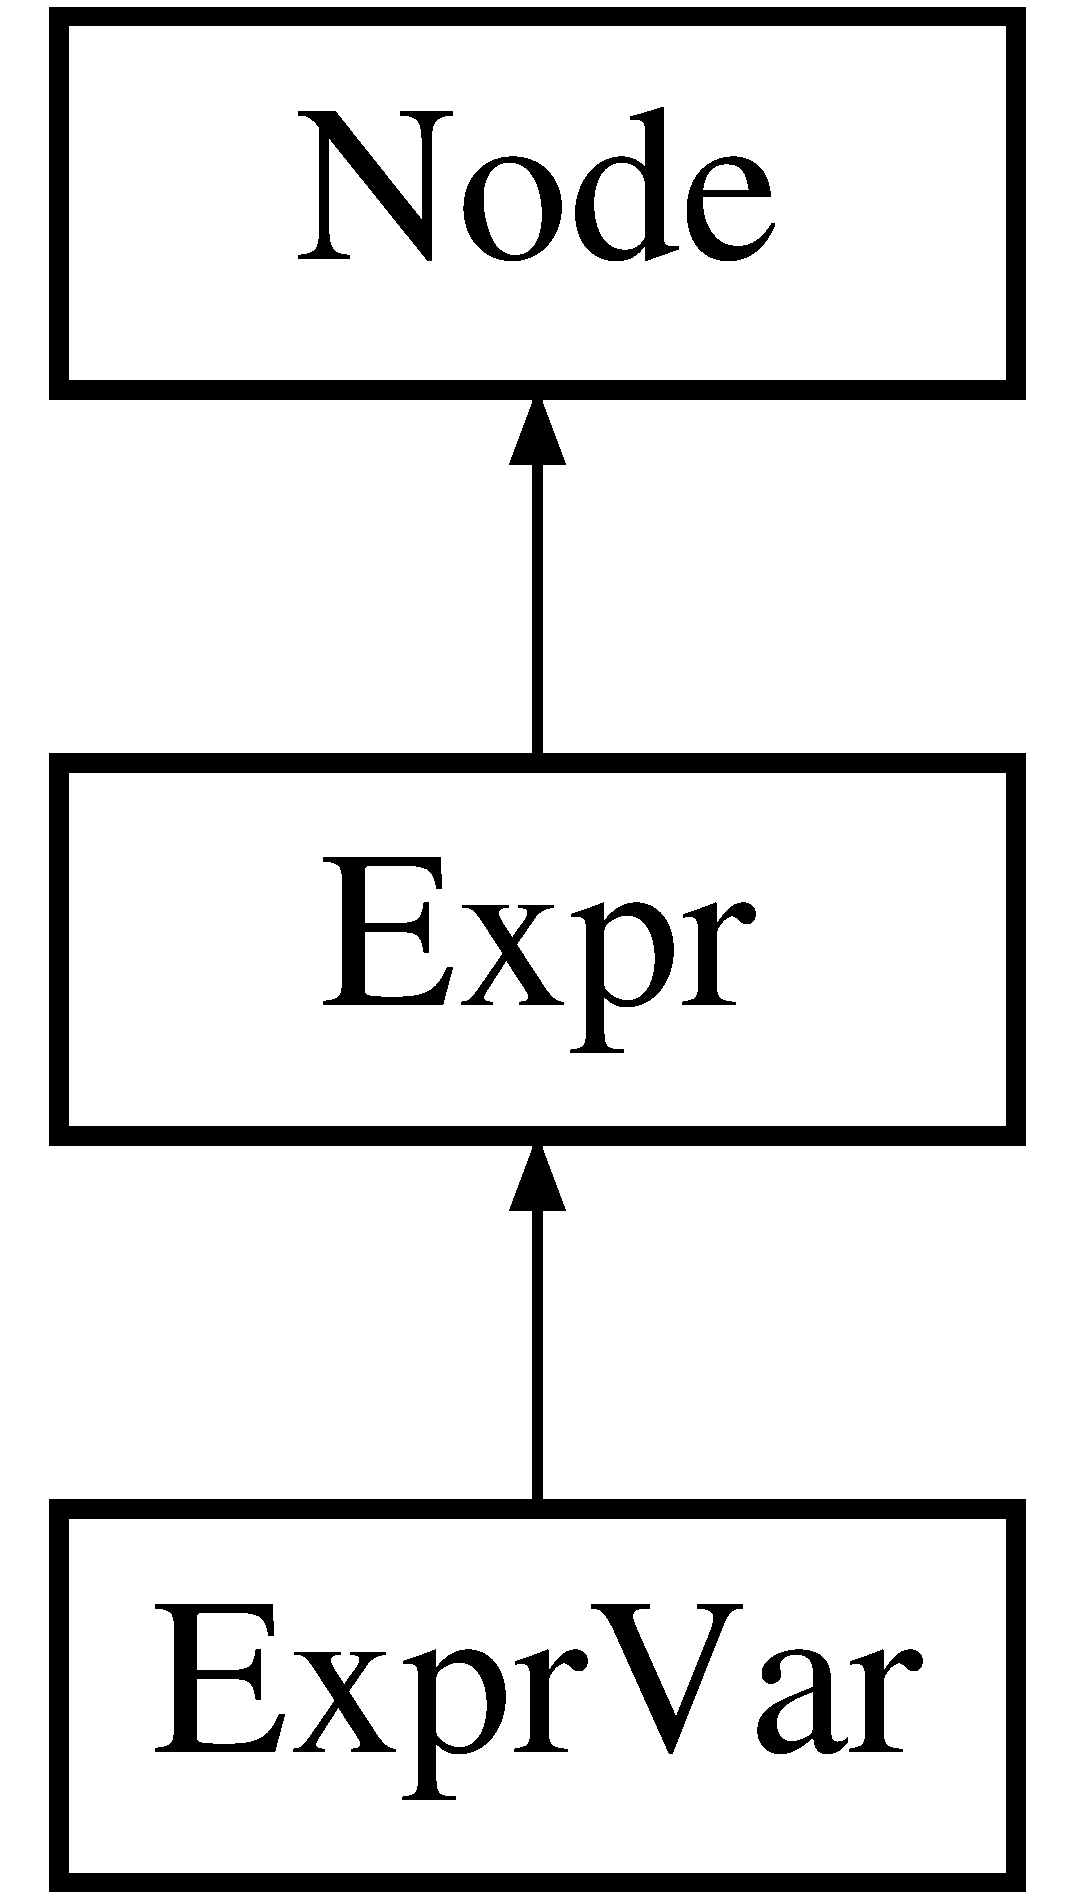
\includegraphics[height=3.000000cm]{classExprVar}
\end{center}
\end{figure}
\subsection*{Public Member Functions}
\begin{DoxyCompactItemize}
\item 
\hypertarget{classExprVar_a1d364d77e8a4eba1ed3c546602b17157}{{\bfseries Expr\-Var} (\hyperlink{classVarname}{Varname} $\ast$\-\_\-v)}\label{classExprVar_a1d364d77e8a4eba1ed3c546602b17157}

\item 
\hypertarget{classExprVar_aea5a227b096764682224ea2cec02a05f}{std\-::string {\bfseries unparse} ()}\label{classExprVar_aea5a227b096764682224ea2cec02a05f}

\end{DoxyCompactItemize}


\subsection{Detailed Description}
This class is for a variable name expression 

The documentation for this class was generated from the following files\-:\begin{DoxyCompactItemize}
\item 
A\-S\-T.\-h\item 
A\-S\-T.\-cpp\end{DoxyCompactItemize}

\hypertarget{classExtToken}{\section{Ext\-Token Class Reference}
\label{classExtToken}\index{Ext\-Token@{Ext\-Token}}
}
Inheritance diagram for Ext\-Token\-:\begin{figure}[H]
\begin{center}
\leavevmode
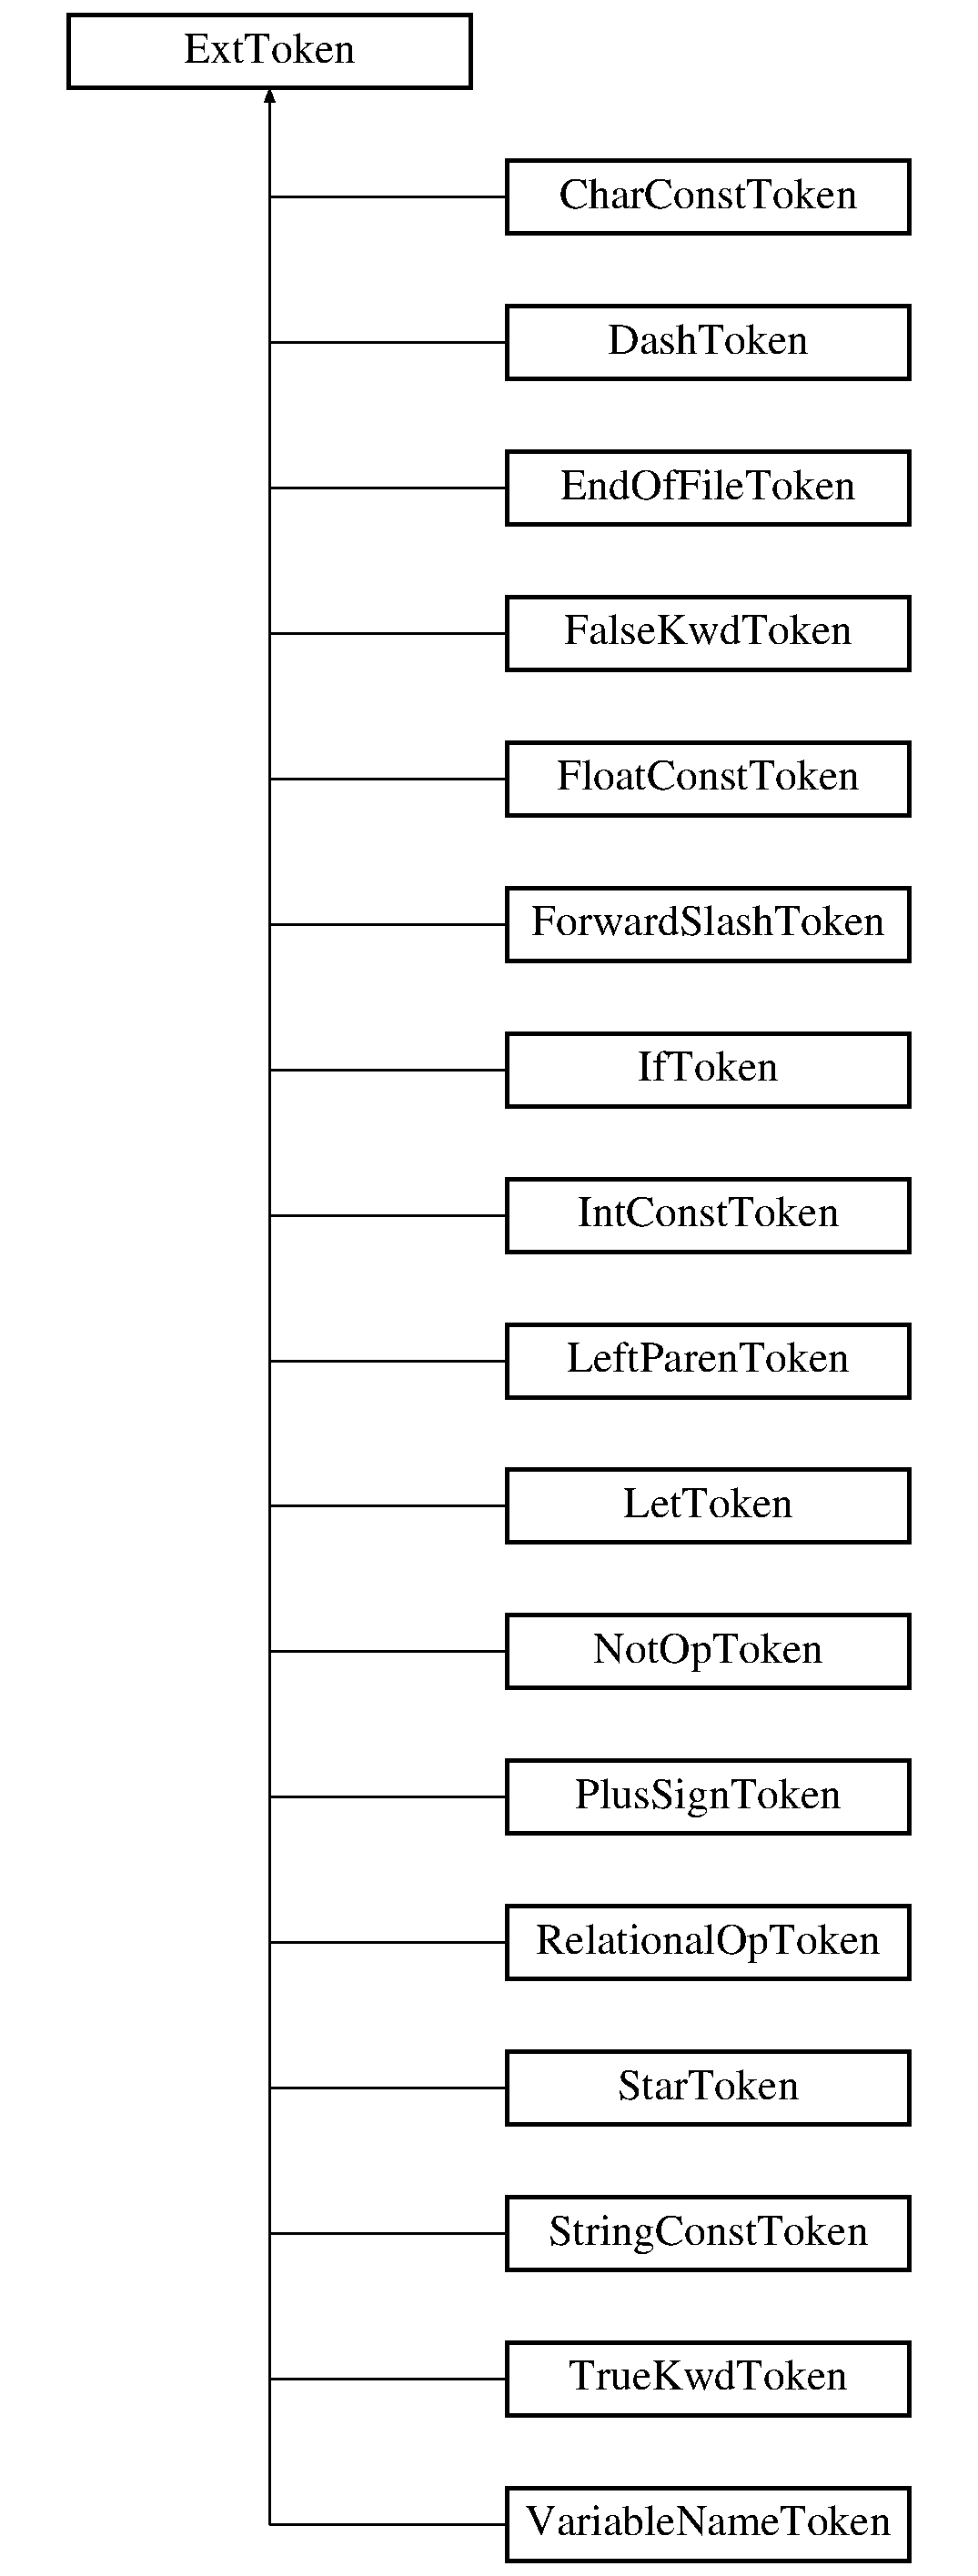
\includegraphics[height=12.000000cm]{classExtToken}
\end{center}
\end{figure}
\subsection*{Public Member Functions}
\begin{DoxyCompactItemize}
\item 
\hypertarget{classExtToken_a45a27528f391faf5679b7b30563ce846}{{\bfseries Ext\-Token} (\hyperlink{classParser}{Parser} $\ast$p, \hyperlink{classToken}{Token} $\ast$t)}\label{classExtToken_a45a27528f391faf5679b7b30563ce846}

\item 
\hypertarget{classExtToken_afa8972152abec42cd52b6f6f70a9a179}{{\bfseries Ext\-Token} (\hyperlink{classParser}{Parser} $\ast$p, \hyperlink{classToken}{Token} $\ast$t, std\-::string d)}\label{classExtToken_afa8972152abec42cd52b6f6f70a9a179}

\item 
\hypertarget{classExtToken_a5c21a5ffe91f212085259126652ab77c}{virtual \hyperlink{classParseResult}{Parse\-Result} {\bfseries nud} ()}\label{classExtToken_a5c21a5ffe91f212085259126652ab77c}

\item 
\hypertarget{classExtToken_afb2c9b0040e198d1d8aa2e041c5a7211}{virtual \hyperlink{classParseResult}{Parse\-Result} {\bfseries led} (\hyperlink{classParseResult}{Parse\-Result} left)}\label{classExtToken_afb2c9b0040e198d1d8aa2e041c5a7211}

\item 
\hypertarget{classExtToken_a6c0d61faa058b71147dd54bacee1db94}{virtual int {\bfseries lbp} ()}\label{classExtToken_a6c0d61faa058b71147dd54bacee1db94}

\item 
\hypertarget{classExtToken_a4ab6e72ac23235650b1756f794172ebb}{virtual std\-::string {\bfseries description} ()}\label{classExtToken_a4ab6e72ac23235650b1756f794172ebb}

\end{DoxyCompactItemize}
\subsection*{Public Attributes}
\begin{DoxyCompactItemize}
\item 
\hypertarget{classExtToken_a5af1643a542ef7ee8ca0f82706383ae3}{std\-::string {\bfseries lexeme}}\label{classExtToken_a5af1643a542ef7ee8ca0f82706383ae3}

\item 
\hypertarget{classExtToken_abbdaef42b65403cdc0247839ef95c875}{token\-Type {\bfseries terminal}}\label{classExtToken_abbdaef42b65403cdc0247839ef95c875}

\item 
\hypertarget{classExtToken_aa02995a897183b2a6ef758e541534e46}{\hyperlink{classExtToken}{Ext\-Token} $\ast$ {\bfseries next}}\label{classExtToken_aa02995a897183b2a6ef758e541534e46}

\item 
\hypertarget{classExtToken_af70d22156d5f8e855a8b0d92a82706ba}{\hyperlink{classParser}{Parser} $\ast$ {\bfseries parser}}\label{classExtToken_af70d22156d5f8e855a8b0d92a82706ba}

\end{DoxyCompactItemize}


The documentation for this class was generated from the following file\-:\begin{DoxyCompactItemize}
\item 
ext\-Token.\-h\end{DoxyCompactItemize}

\hypertarget{classFalseKwdToken}{\section{False\-Kwd\-Token Class Reference}
\label{classFalseKwdToken}\index{False\-Kwd\-Token@{False\-Kwd\-Token}}
}
Inheritance diagram for False\-Kwd\-Token\-:\begin{figure}[H]
\begin{center}
\leavevmode
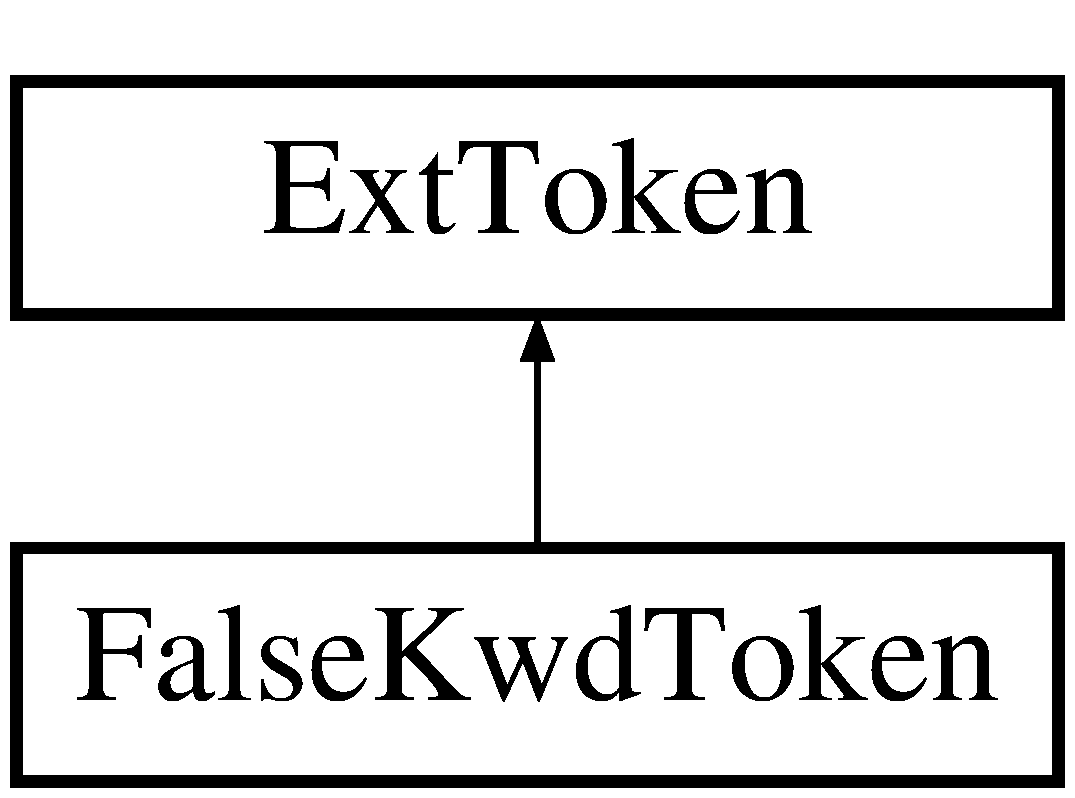
\includegraphics[height=2.000000cm]{classFalseKwdToken}
\end{center}
\end{figure}
\subsection*{Public Member Functions}
\begin{DoxyCompactItemize}
\item 
\hypertarget{classFalseKwdToken_add6402d29fd7b22253a0dc73370597e4}{{\bfseries False\-Kwd\-Token} (\hyperlink{classParser}{Parser} $\ast$p, \hyperlink{classToken}{Token} $\ast$t)}\label{classFalseKwdToken_add6402d29fd7b22253a0dc73370597e4}

\item 
\hypertarget{classFalseKwdToken_adc06b0433535d552c1e7f8076d756fb3}{\hyperlink{classParseResult}{Parse\-Result} {\bfseries nud} ()}\label{classFalseKwdToken_adc06b0433535d552c1e7f8076d756fb3}

\item 
\hypertarget{classFalseKwdToken_a8351fad7090214687138e113b5a581f1}{std\-::string {\bfseries description} ()}\label{classFalseKwdToken_a8351fad7090214687138e113b5a581f1}

\end{DoxyCompactItemize}
\subsection*{Additional Inherited Members}


The documentation for this class was generated from the following file\-:\begin{DoxyCompactItemize}
\item 
ext\-Token.\-h\end{DoxyCompactItemize}

\hypertarget{classFloatConstToken}{\section{Float\-Const\-Token Class Reference}
\label{classFloatConstToken}\index{Float\-Const\-Token@{Float\-Const\-Token}}
}
Inheritance diagram for Float\-Const\-Token\-:\begin{figure}[H]
\begin{center}
\leavevmode
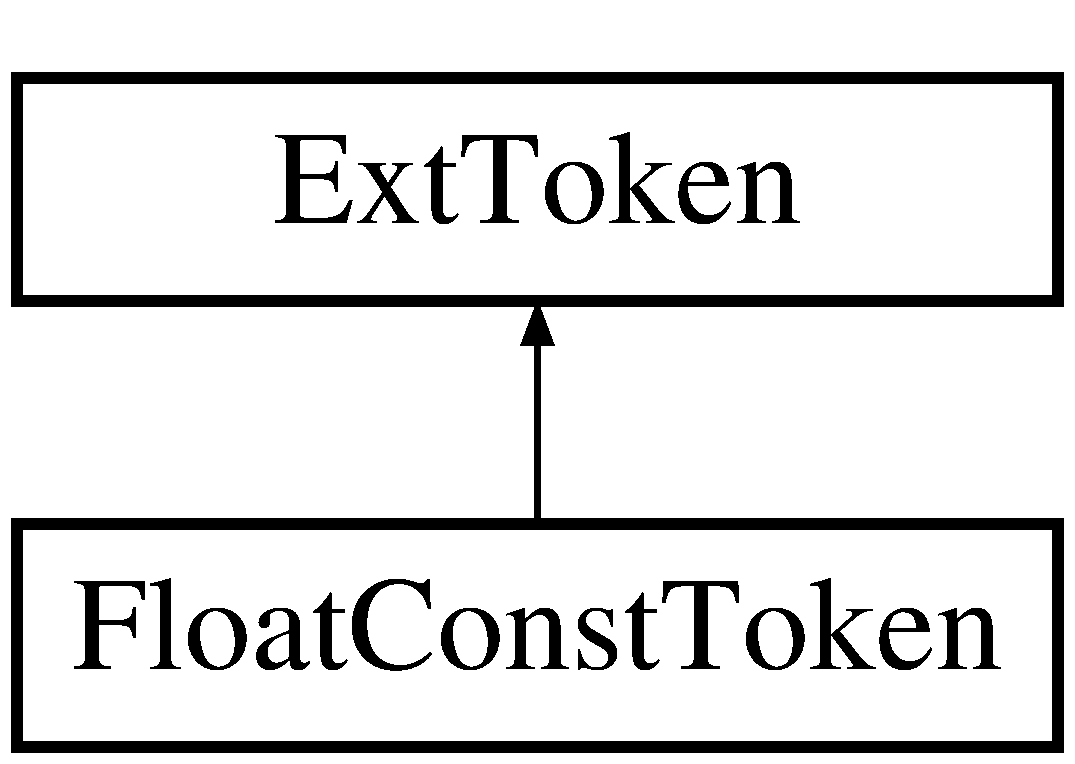
\includegraphics[height=2.000000cm]{classFloatConstToken}
\end{center}
\end{figure}
\subsection*{Public Member Functions}
\begin{DoxyCompactItemize}
\item 
\hypertarget{classFloatConstToken_aecee1d0e4e8a9410701c68c30858a4db}{{\bfseries Float\-Const\-Token} (\hyperlink{classParser}{Parser} $\ast$p, \hyperlink{classToken}{Token} $\ast$t)}\label{classFloatConstToken_aecee1d0e4e8a9410701c68c30858a4db}

\item 
\hypertarget{classFloatConstToken_a991e92ae34d0b01a3b1dd08ed01b8e6e}{\hyperlink{classParseResult}{Parse\-Result} {\bfseries nud} ()}\label{classFloatConstToken_a991e92ae34d0b01a3b1dd08ed01b8e6e}

\item 
\hypertarget{classFloatConstToken_a529b6d3ad479b0f6b940a82ba48b98c0}{std\-::string {\bfseries description} ()}\label{classFloatConstToken_a529b6d3ad479b0f6b940a82ba48b98c0}

\end{DoxyCompactItemize}
\subsection*{Additional Inherited Members}


The documentation for this class was generated from the following file\-:\begin{DoxyCompactItemize}
\item 
ext\-Token.\-h\end{DoxyCompactItemize}

\hypertarget{classForwardSlashToken}{\section{Forward\-Slash\-Token Class Reference}
\label{classForwardSlashToken}\index{Forward\-Slash\-Token@{Forward\-Slash\-Token}}
}
Inheritance diagram for Forward\-Slash\-Token\-:\begin{figure}[H]
\begin{center}
\leavevmode
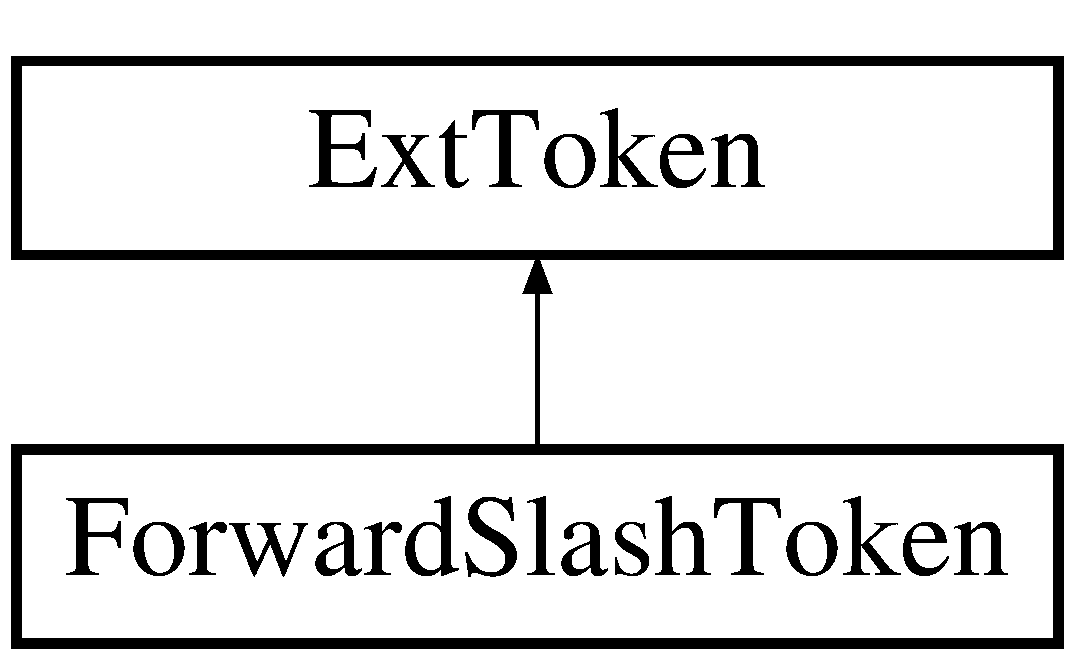
\includegraphics[height=2.000000cm]{classForwardSlashToken}
\end{center}
\end{figure}
\subsection*{Public Member Functions}
\begin{DoxyCompactItemize}
\item 
\hypertarget{classForwardSlashToken_ae818840269cd15f6f6b00929fb4eb979}{{\bfseries Forward\-Slash\-Token} (\hyperlink{classParser}{Parser} $\ast$p, \hyperlink{classToken}{Token} $\ast$t)}\label{classForwardSlashToken_ae818840269cd15f6f6b00929fb4eb979}

\item 
\hypertarget{classForwardSlashToken_ac2dda7b791ab555e4323f17baaf323e1}{\hyperlink{classParseResult}{Parse\-Result} {\bfseries led} (\hyperlink{classParseResult}{Parse\-Result} left)}\label{classForwardSlashToken_ac2dda7b791ab555e4323f17baaf323e1}

\item 
\hypertarget{classForwardSlashToken_ac27b1ab175ec08c468bd0d4c41636a5c}{std\-::string {\bfseries description} ()}\label{classForwardSlashToken_ac27b1ab175ec08c468bd0d4c41636a5c}

\item 
\hypertarget{classForwardSlashToken_ad65829044355922a291dfbfd3052b183}{int {\bfseries lbp} ()}\label{classForwardSlashToken_ad65829044355922a291dfbfd3052b183}

\end{DoxyCompactItemize}
\subsection*{Additional Inherited Members}


The documentation for this class was generated from the following file\-:\begin{DoxyCompactItemize}
\item 
ext\-Token.\-h\end{DoxyCompactItemize}

\hypertarget{classIfExpr}{\section{If\-Expr Class Reference}
\label{classIfExpr}\index{If\-Expr@{If\-Expr}}
}


{\ttfamily \#include $<$A\-S\-T.\-h$>$}

Inheritance diagram for If\-Expr\-:\begin{figure}[H]
\begin{center}
\leavevmode
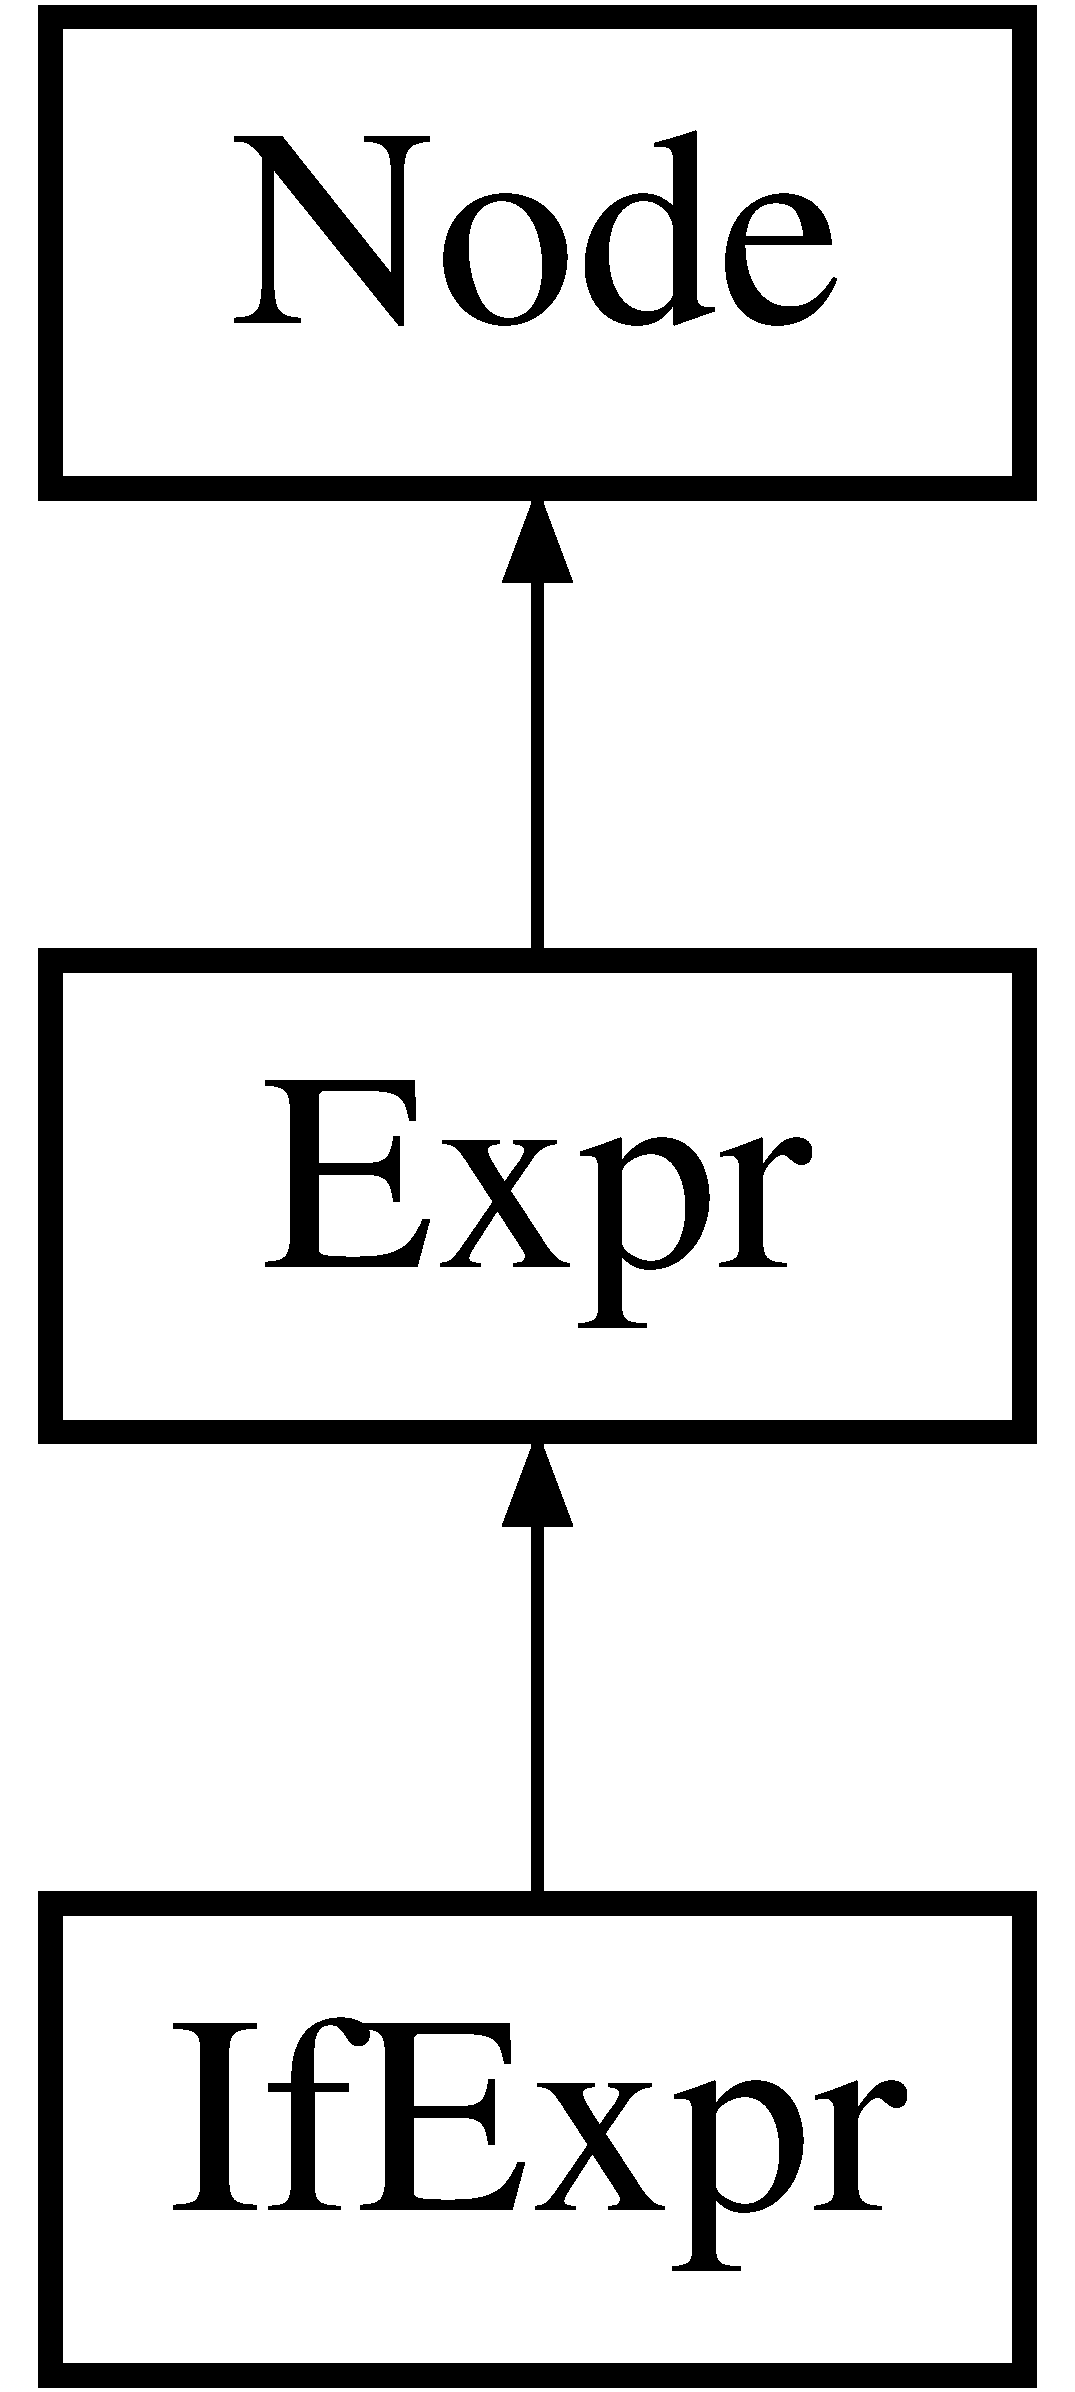
\includegraphics[height=3.000000cm]{classIfExpr}
\end{center}
\end{figure}
\subsection*{Public Member Functions}
\begin{DoxyCompactItemize}
\item 
\hypertarget{classIfExpr_a3c49b1c3aea31559e36e8fb6443726ed}{{\bfseries If\-Expr} (\hyperlink{classExpr}{Expr} $\ast$\-\_\-e, \hyperlink{classExpr}{Expr} $\ast$\-\_\-left, \hyperlink{classExpr}{Expr} $\ast$\-\_\-right)}\label{classIfExpr_a3c49b1c3aea31559e36e8fb6443726ed}

\item 
\hypertarget{classIfExpr_a49667b0be8ad229abbd8666fea195028}{std\-::string {\bfseries unparse} ()}\label{classIfExpr_a49667b0be8ad229abbd8666fea195028}

\end{DoxyCompactItemize}


\subsection{Detailed Description}
This class is for an if-\/then-\/else expression 

The documentation for this class was generated from the following file\-:\begin{DoxyCompactItemize}
\item 
A\-S\-T.\-h\end{DoxyCompactItemize}

\hypertarget{classIfToken}{\section{If\-Token Class Reference}
\label{classIfToken}\index{If\-Token@{If\-Token}}
}
Inheritance diagram for If\-Token\-:\begin{figure}[H]
\begin{center}
\leavevmode
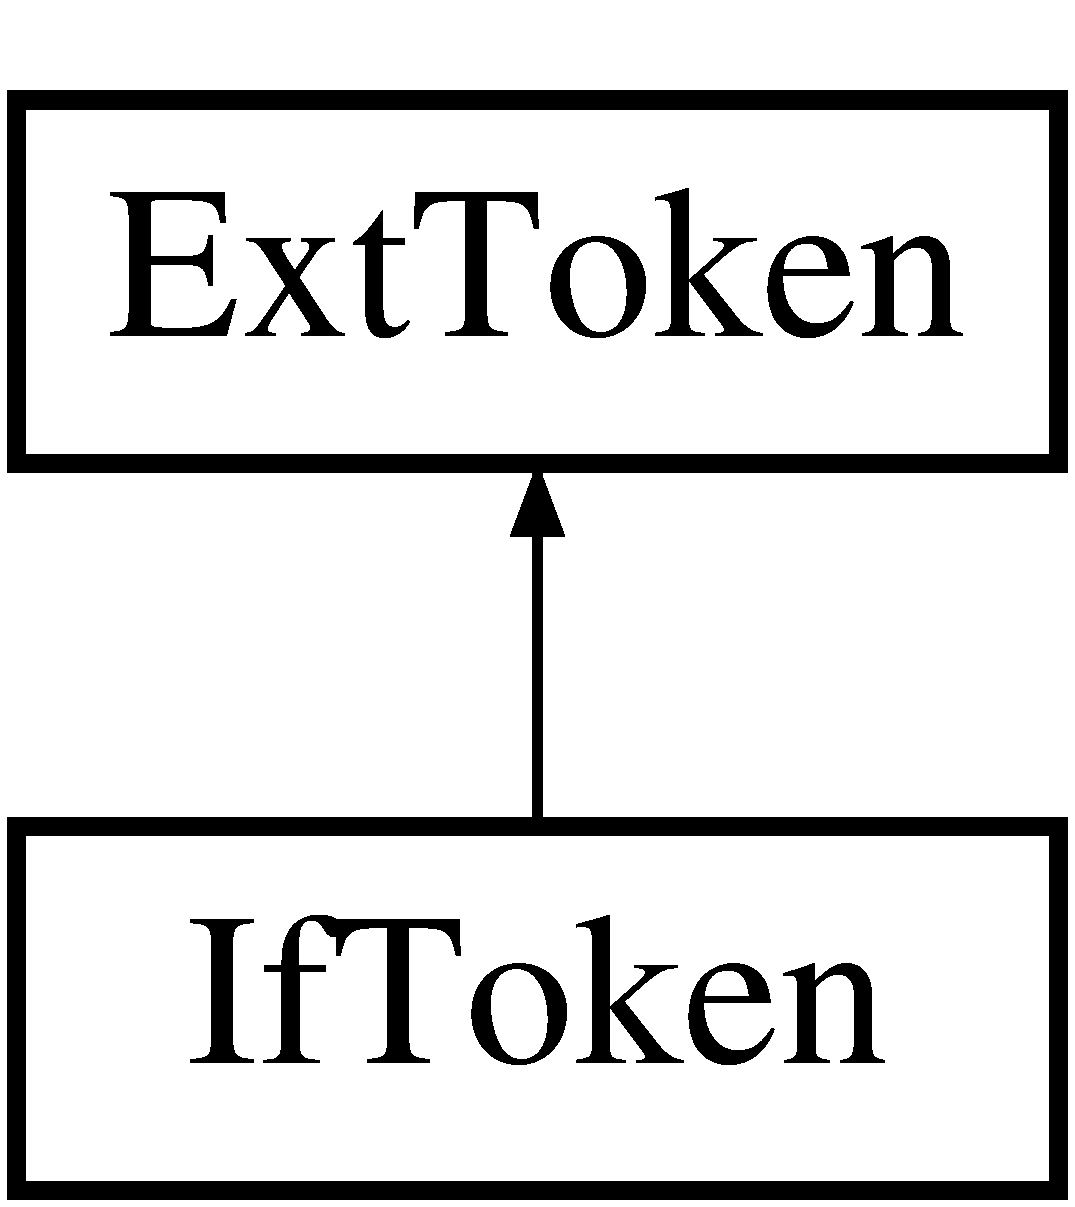
\includegraphics[height=2.000000cm]{classIfToken}
\end{center}
\end{figure}
\subsection*{Public Member Functions}
\begin{DoxyCompactItemize}
\item 
\hypertarget{classIfToken_a607028595b06b8a950000ba3e82329db}{{\bfseries If\-Token} (\hyperlink{classParser}{Parser} $\ast$p, \hyperlink{classToken}{Token} $\ast$t)}\label{classIfToken_a607028595b06b8a950000ba3e82329db}

\item 
\hypertarget{classIfToken_add06bd79ce755fd5503f78e507109e52}{\hyperlink{classParseResult}{Parse\-Result} {\bfseries nud} ()}\label{classIfToken_add06bd79ce755fd5503f78e507109e52}

\item 
\hypertarget{classIfToken_aad226162c5649920c13c2a9e9e7a3617}{std\-::string {\bfseries description} ()}\label{classIfToken_aad226162c5649920c13c2a9e9e7a3617}

\item 
\hypertarget{classIfToken_abfd39ff4c4818d382bf0b97fd097c478}{int {\bfseries lbp} ()}\label{classIfToken_abfd39ff4c4818d382bf0b97fd097c478}

\end{DoxyCompactItemize}
\subsection*{Additional Inherited Members}


The documentation for this class was generated from the following file\-:\begin{DoxyCompactItemize}
\item 
ext\-Token.\-h\end{DoxyCompactItemize}

\hypertarget{classIntConstToken}{\section{Int\-Const\-Token Class Reference}
\label{classIntConstToken}\index{Int\-Const\-Token@{Int\-Const\-Token}}
}
Inheritance diagram for Int\-Const\-Token\-:\begin{figure}[H]
\begin{center}
\leavevmode
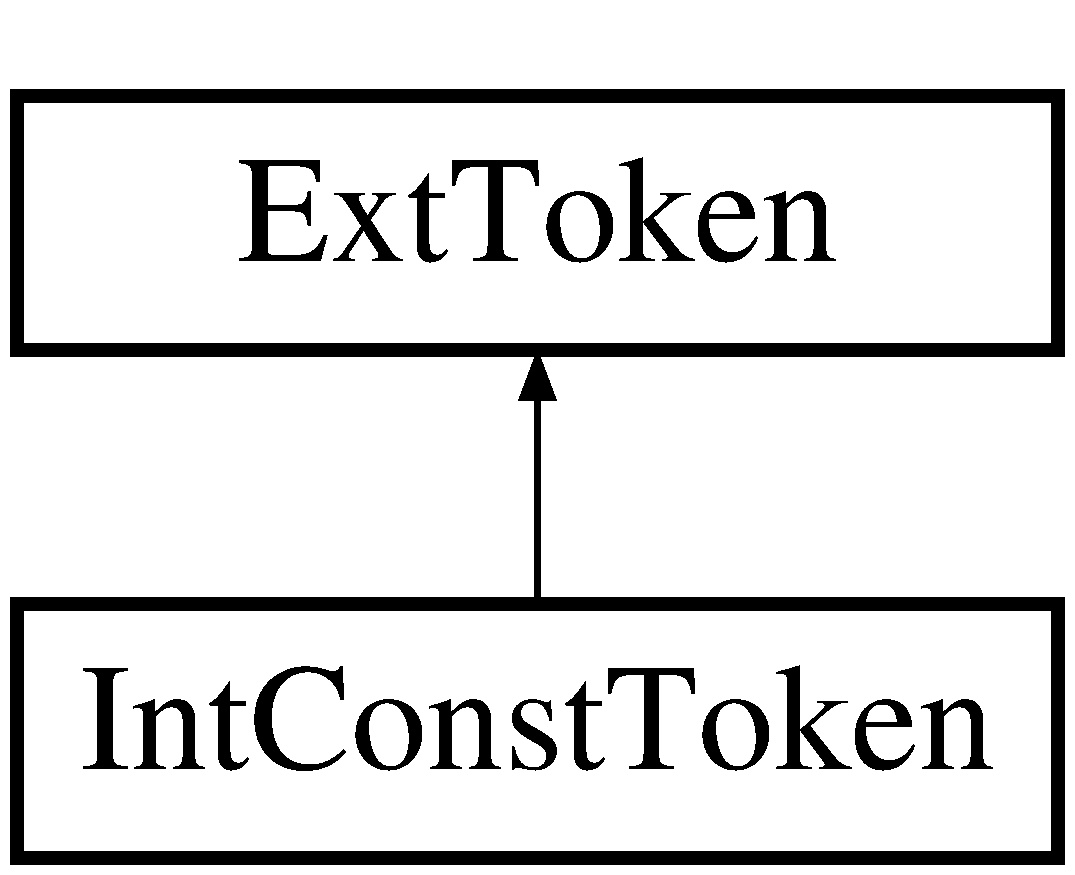
\includegraphics[height=2.000000cm]{classIntConstToken}
\end{center}
\end{figure}
\subsection*{Public Member Functions}
\begin{DoxyCompactItemize}
\item 
\hypertarget{classIntConstToken_a14c6bf0af5a915969b4fef1758067af3}{{\bfseries Int\-Const\-Token} (\hyperlink{classParser}{Parser} $\ast$p, \hyperlink{classToken}{Token} $\ast$t)}\label{classIntConstToken_a14c6bf0af5a915969b4fef1758067af3}

\item 
\hypertarget{classIntConstToken_ae1f720d6006c47e145cae7879d09c708}{\hyperlink{classParseResult}{Parse\-Result} {\bfseries nud} ()}\label{classIntConstToken_ae1f720d6006c47e145cae7879d09c708}

\item 
\hypertarget{classIntConstToken_a98191508d849878d40800e447a0f1892}{std\-::string {\bfseries description} ()}\label{classIntConstToken_a98191508d849878d40800e447a0f1892}

\end{DoxyCompactItemize}
\subsection*{Additional Inherited Members}


The documentation for this class was generated from the following file\-:\begin{DoxyCompactItemize}
\item 
ext\-Token.\-h\end{DoxyCompactItemize}

\hypertarget{classKwdDecl}{\section{Kwd\-Decl Class Reference}
\label{classKwdDecl}\index{Kwd\-Decl@{Kwd\-Decl}}
}


{\ttfamily \#include $<$A\-S\-T.\-h$>$}

Inheritance diagram for Kwd\-Decl\-:\begin{figure}[H]
\begin{center}
\leavevmode
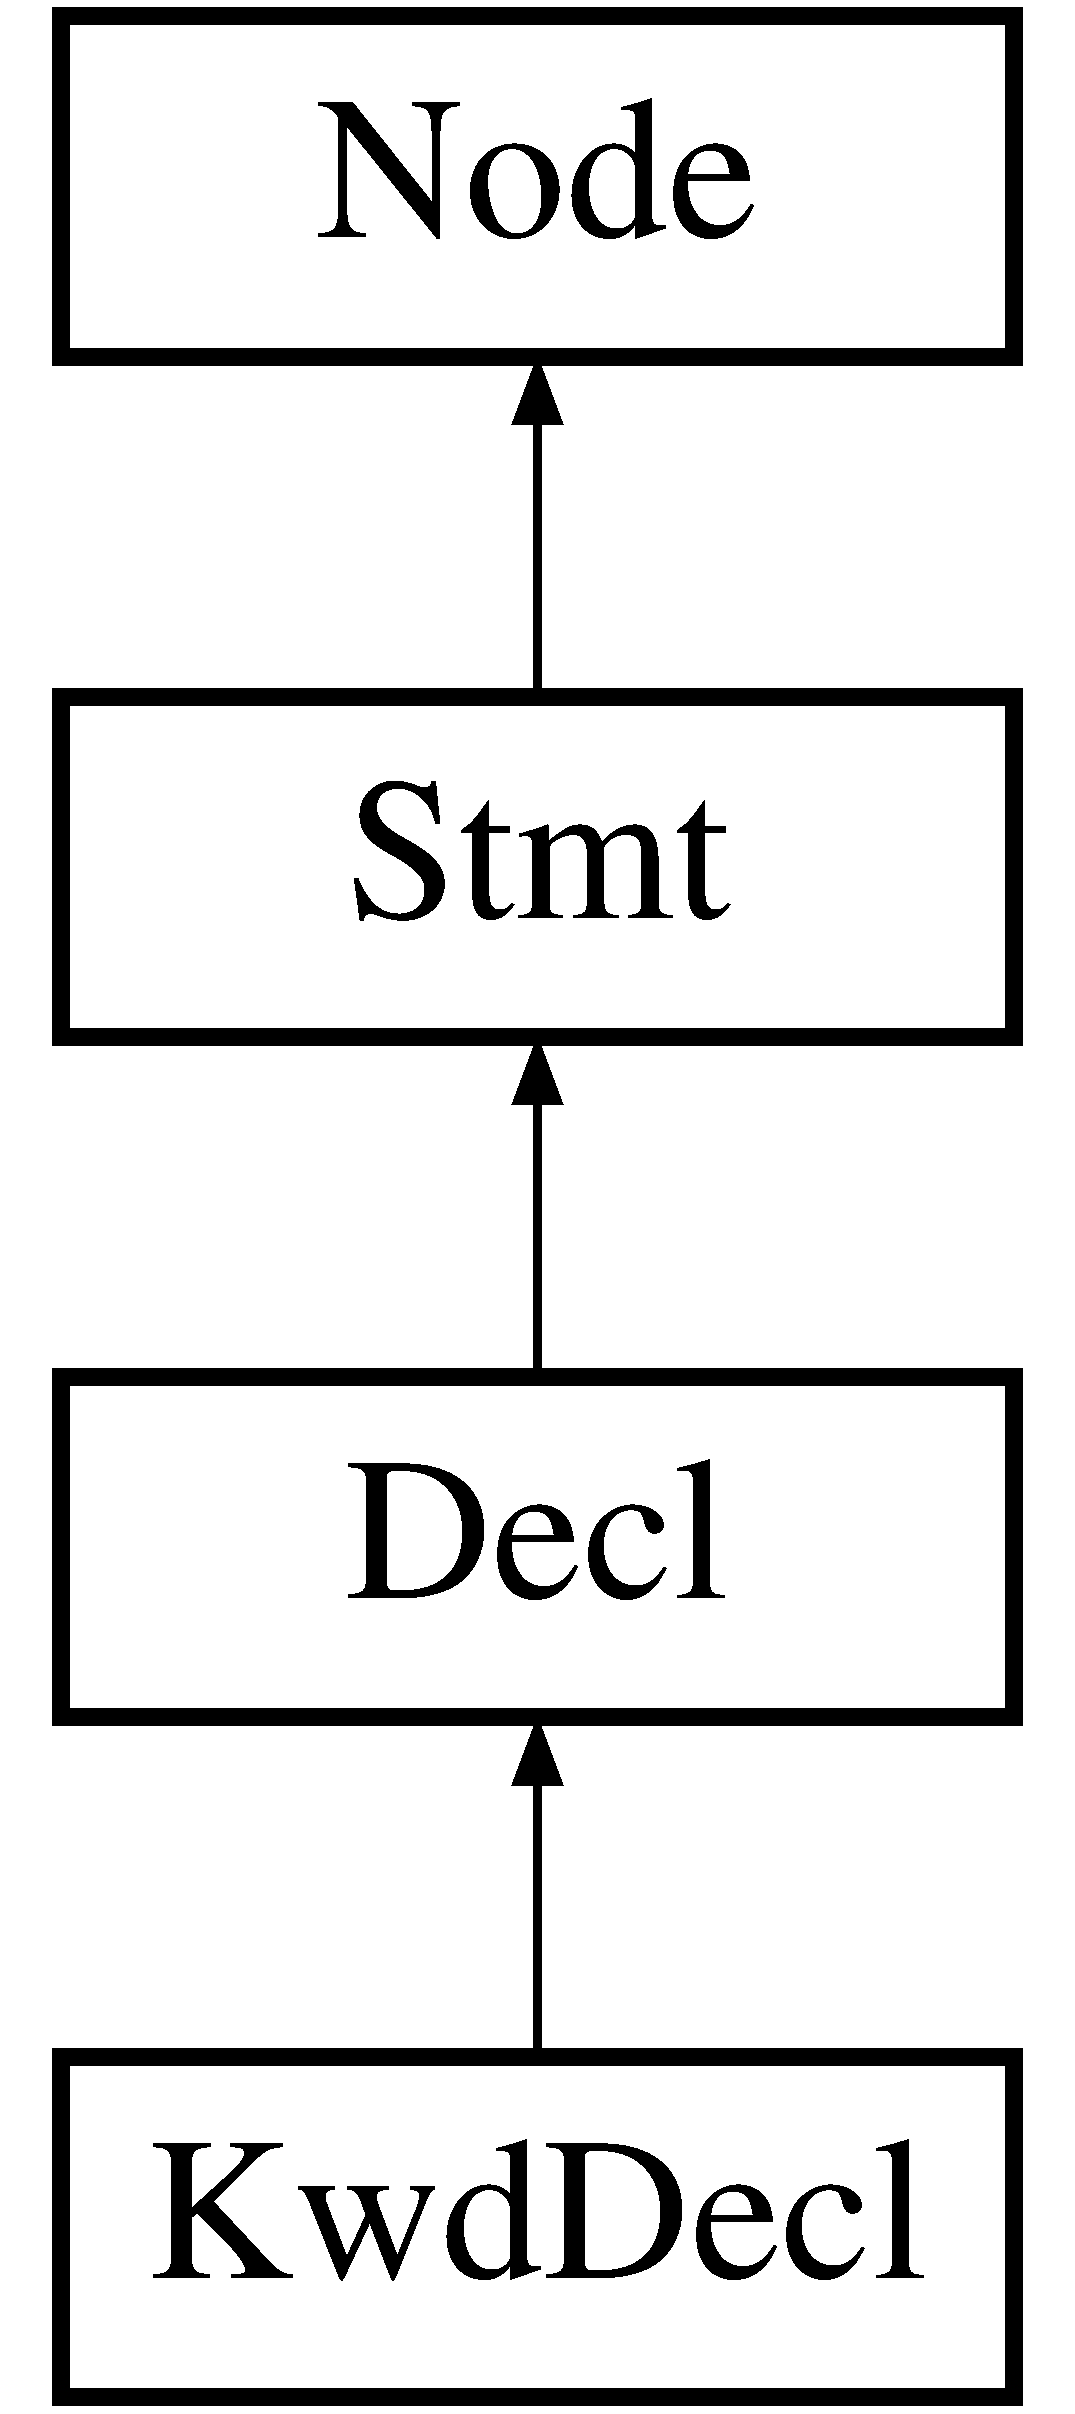
\includegraphics[height=4.000000cm]{classKwdDecl}
\end{center}
\end{figure}
\subsection*{Public Member Functions}
\begin{DoxyCompactItemize}
\item 
\hypertarget{classKwdDecl_a676b9e05697b0acf311b3c57456d7304}{{\bfseries Kwd\-Decl} (token\-Type \-\_\-kwd, \hyperlink{classVarname}{Varname} $\ast$\-\_\-varname)}\label{classKwdDecl_a676b9e05697b0acf311b3c57456d7304}

\item 
\hypertarget{classKwdDecl_ac5f258785ee2a869413772b32c627973}{std\-::string {\bfseries unparse} ()}\label{classKwdDecl_ac5f258785ee2a869413772b32c627973}

\end{DoxyCompactItemize}


\subsection{Detailed Description}
This class is for a keyword declaration, like Int q or anything else  use this for all 4 keyword because they are essentially all similarly implemented (string as the keyword) 

The documentation for this class was generated from the following files\-:\begin{DoxyCompactItemize}
\item 
A\-S\-T.\-h\item 
A\-S\-T.\-cpp\end{DoxyCompactItemize}

\hypertarget{classLeftParenToken}{\section{Left\-Paren\-Token Class Reference}
\label{classLeftParenToken}\index{Left\-Paren\-Token@{Left\-Paren\-Token}}
}
Inheritance diagram for Left\-Paren\-Token\-:\begin{figure}[H]
\begin{center}
\leavevmode
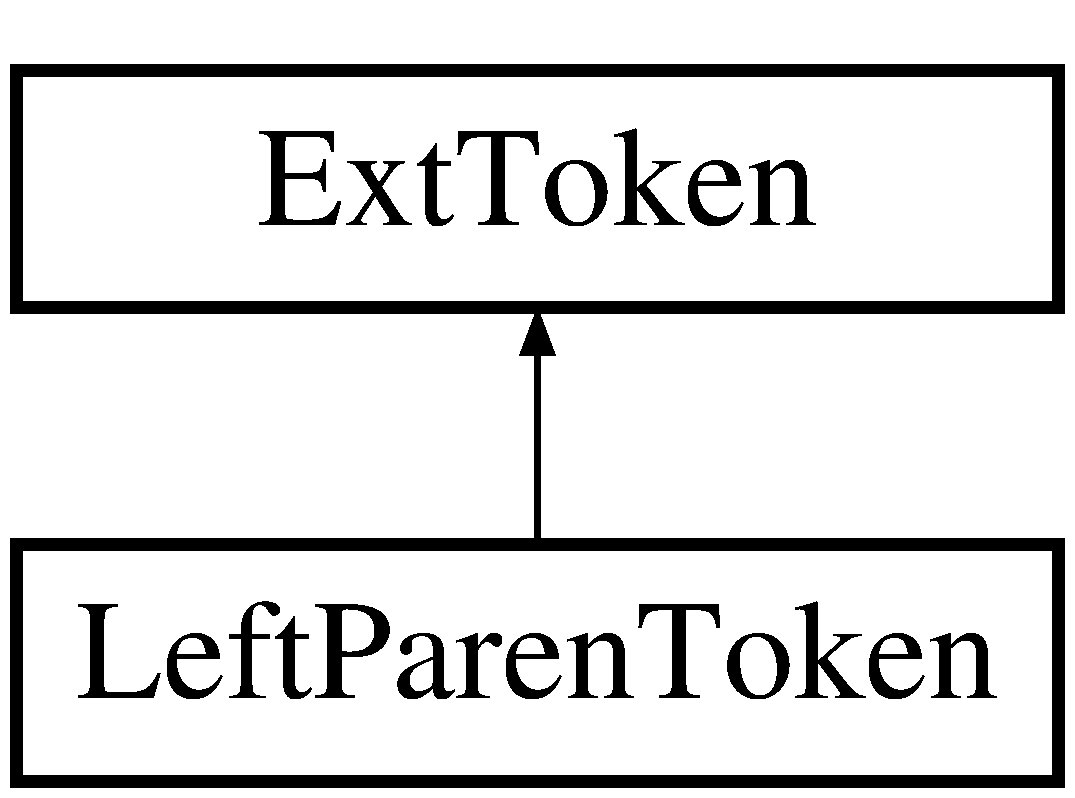
\includegraphics[height=2.000000cm]{classLeftParenToken}
\end{center}
\end{figure}
\subsection*{Public Member Functions}
\begin{DoxyCompactItemize}
\item 
\hypertarget{classLeftParenToken_aecdc6faf48a1a7192ec55712f0264cba}{{\bfseries Left\-Paren\-Token} (\hyperlink{classParser}{Parser} $\ast$p, \hyperlink{classToken}{Token} $\ast$t)}\label{classLeftParenToken_aecdc6faf48a1a7192ec55712f0264cba}

\item 
\hypertarget{classLeftParenToken_a3cb3ae9ab2647e5534c85529d314f08b}{\hyperlink{classParseResult}{Parse\-Result} {\bfseries nud} ()}\label{classLeftParenToken_a3cb3ae9ab2647e5534c85529d314f08b}

\item 
\hypertarget{classLeftParenToken_a2df35684bd2081c3bdfe2357946917bc}{std\-::string {\bfseries description} ()}\label{classLeftParenToken_a2df35684bd2081c3bdfe2357946917bc}

\item 
\hypertarget{classLeftParenToken_afa1b94645278f097bb097d3b24445d14}{int {\bfseries lbp} ()}\label{classLeftParenToken_afa1b94645278f097bb097d3b24445d14}

\end{DoxyCompactItemize}
\subsection*{Additional Inherited Members}


The documentation for this class was generated from the following file\-:\begin{DoxyCompactItemize}
\item 
ext\-Token.\-h\end{DoxyCompactItemize}

\hypertarget{classLetExpr}{\section{Let\-Expr Class Reference}
\label{classLetExpr}\index{Let\-Expr@{Let\-Expr}}
}


{\ttfamily \#include $<$A\-S\-T.\-h$>$}

Inheritance diagram for Let\-Expr\-:\begin{figure}[H]
\begin{center}
\leavevmode
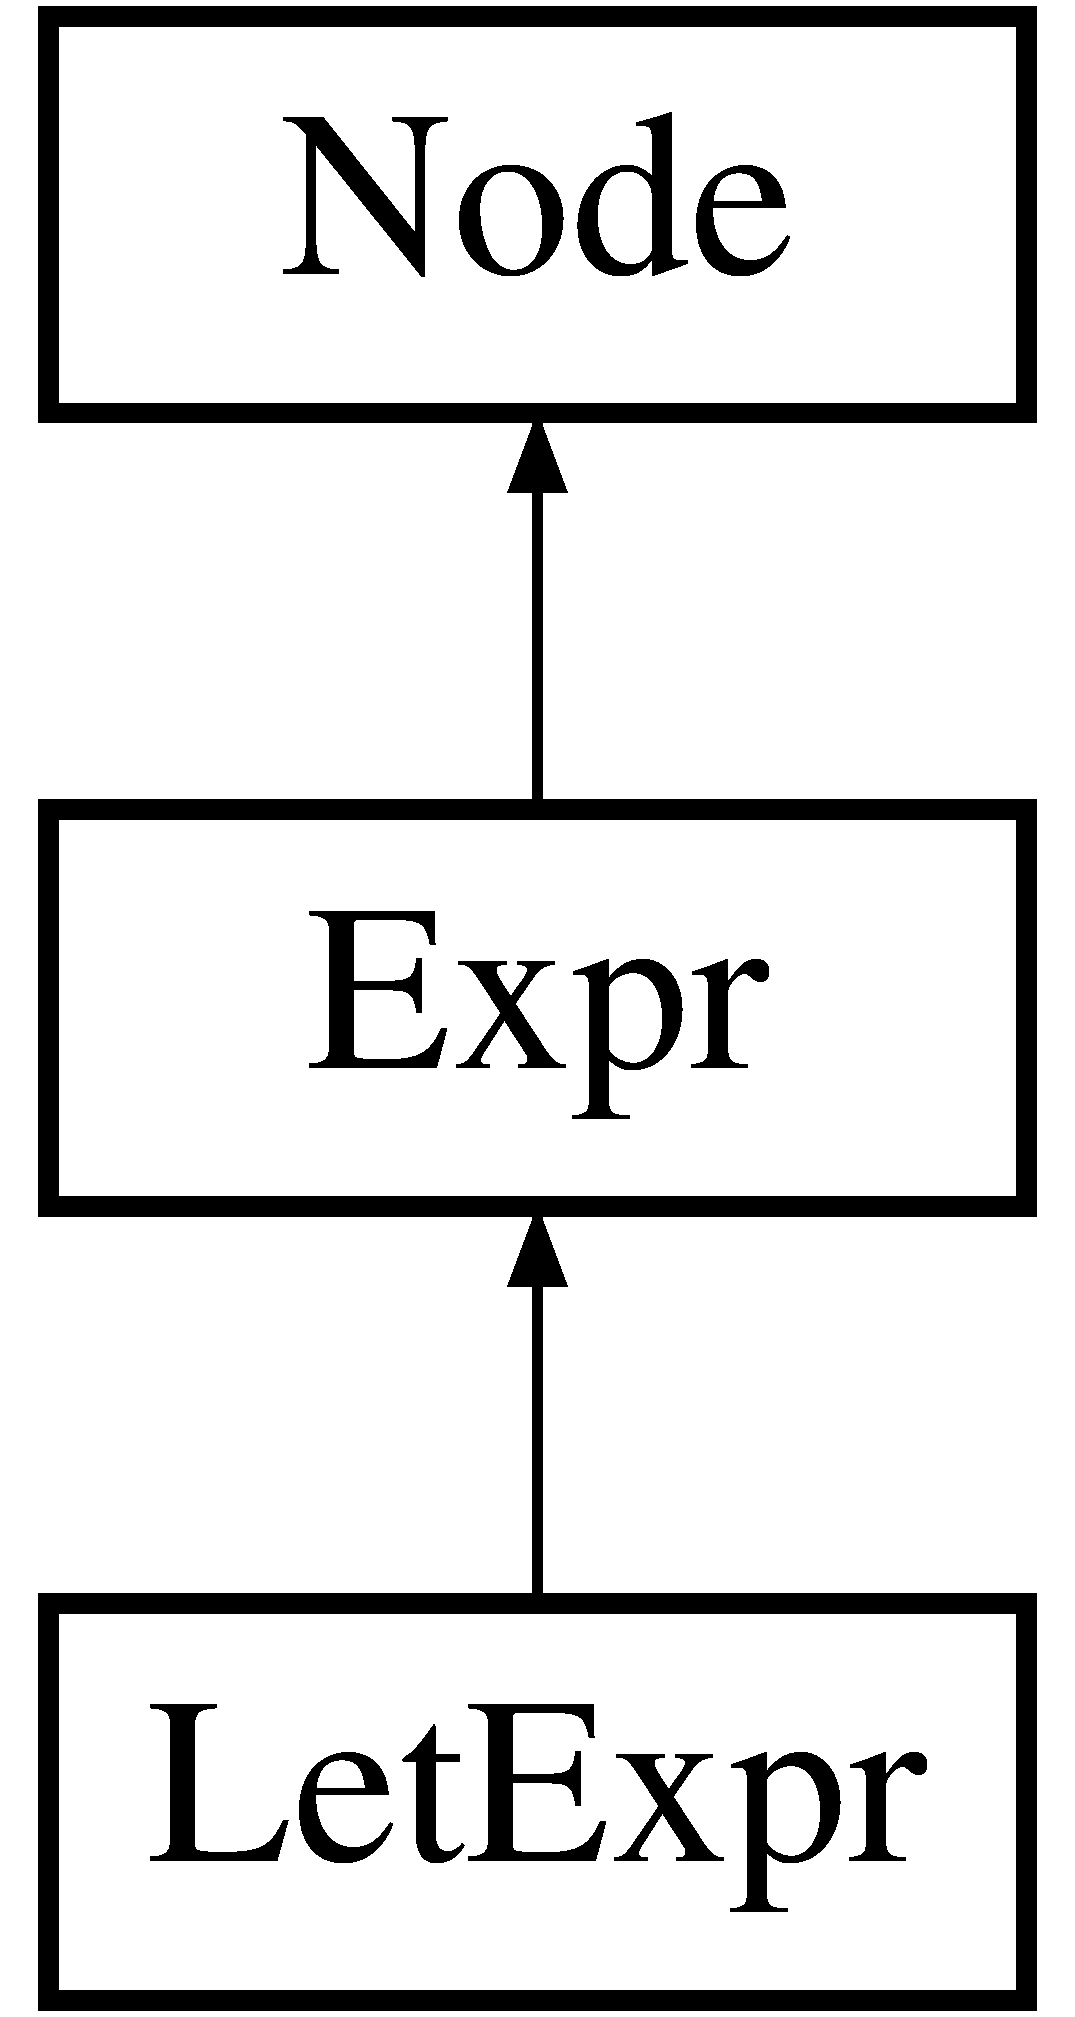
\includegraphics[height=3.000000cm]{classLetExpr}
\end{center}
\end{figure}
\subsection*{Public Member Functions}
\begin{DoxyCompactItemize}
\item 
\hypertarget{classLetExpr_a738f5ec4b4bca67ed0a285891c184f6f}{{\bfseries Let\-Expr} (\hyperlink{classStmts}{Stmts} $\ast$\-\_\-s, \hyperlink{classExpr}{Expr} $\ast$\-\_\-expr)}\label{classLetExpr_a738f5ec4b4bca67ed0a285891c184f6f}

\item 
\hypertarget{classLetExpr_a47e9e62ebec3114d50c127223fff126b}{std\-::string {\bfseries unparse} ()}\label{classLetExpr_a47e9e62ebec3114d50c127223fff126b}

\end{DoxyCompactItemize}


\subsection{Detailed Description}
This class is for a let expression 

The documentation for this class was generated from the following files\-:\begin{DoxyCompactItemize}
\item 
A\-S\-T.\-h\item 
A\-S\-T.\-cpp\end{DoxyCompactItemize}

\hypertarget{classLetToken}{\section{Let\-Token Class Reference}
\label{classLetToken}\index{Let\-Token@{Let\-Token}}
}
Inheritance diagram for Let\-Token\-:\begin{figure}[H]
\begin{center}
\leavevmode
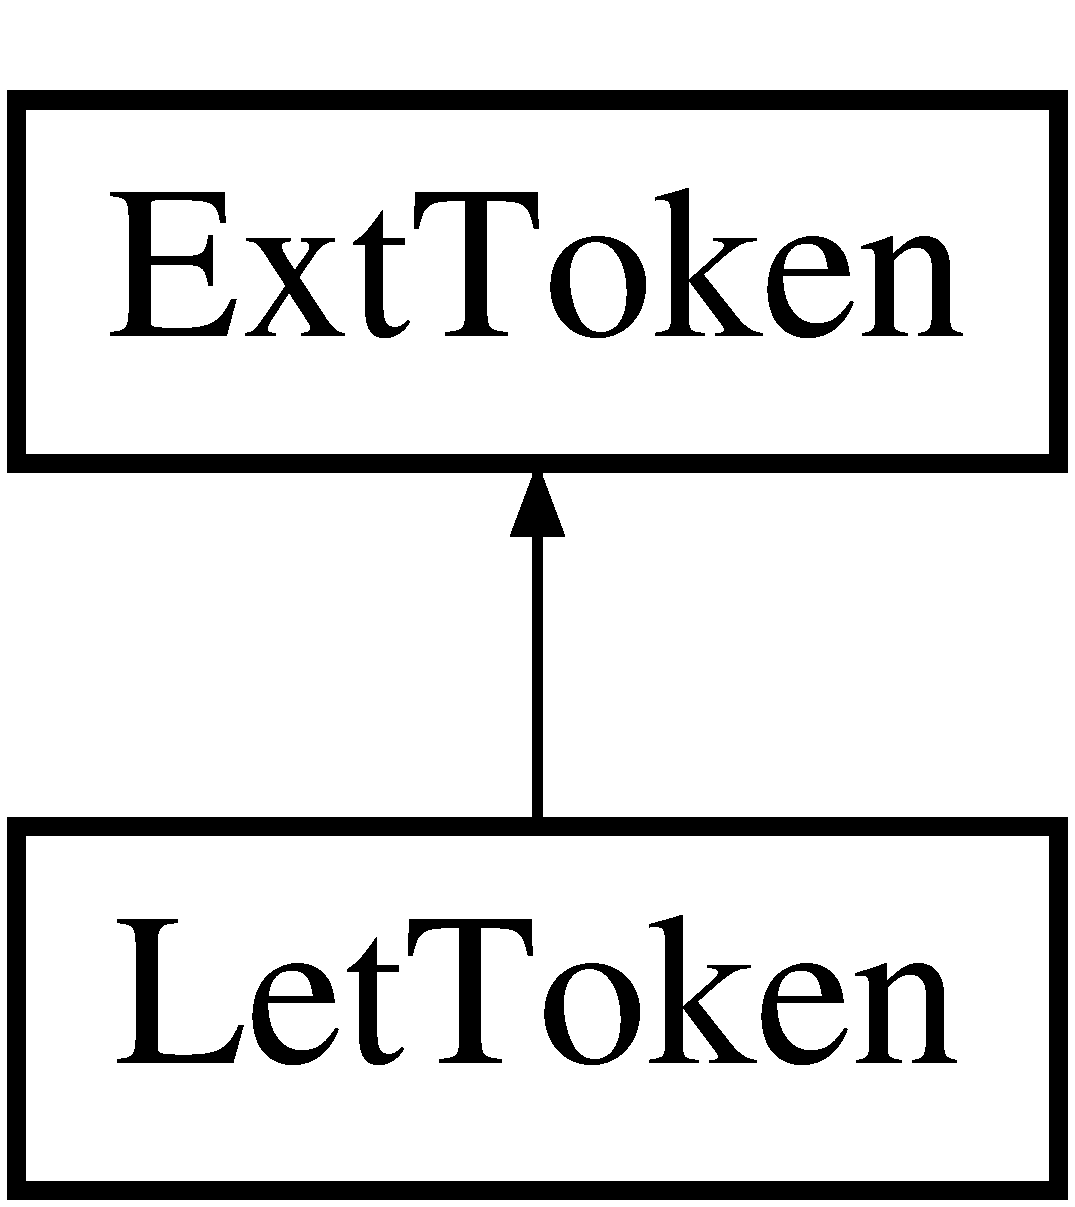
\includegraphics[height=2.000000cm]{classLetToken}
\end{center}
\end{figure}
\subsection*{Public Member Functions}
\begin{DoxyCompactItemize}
\item 
\hypertarget{classLetToken_a94651a82207e47cd2c1066a58cb1fe08}{{\bfseries Let\-Token} (\hyperlink{classParser}{Parser} $\ast$p, \hyperlink{classToken}{Token} $\ast$t)}\label{classLetToken_a94651a82207e47cd2c1066a58cb1fe08}

\item 
\hypertarget{classLetToken_a14df948cdf775bde8392bf58d53b91f3}{\hyperlink{classParseResult}{Parse\-Result} {\bfseries nud} ()}\label{classLetToken_a14df948cdf775bde8392bf58d53b91f3}

\item 
\hypertarget{classLetToken_a2c5ba0489774bf6468a26f4e19d7fab4}{std\-::string {\bfseries description} ()}\label{classLetToken_a2c5ba0489774bf6468a26f4e19d7fab4}

\item 
\hypertarget{classLetToken_a2a5ab5bc5897340513480c162bb2b065}{int {\bfseries lbp} ()}\label{classLetToken_a2a5ab5bc5897340513480c162bb2b065}

\end{DoxyCompactItemize}
\subsection*{Additional Inherited Members}


The documentation for this class was generated from the following file\-:\begin{DoxyCompactItemize}
\item 
ext\-Token.\-h\end{DoxyCompactItemize}

\hypertarget{classmysequence}{\section{mysequence$<$ T, N $>$ Class Template Reference}
\label{classmysequence}\index{mysequence$<$ T, N $>$@{mysequence$<$ T, N $>$}}
}
\subsection*{Public Member Functions}
\begin{DoxyCompactItemize}
\item 
\hypertarget{classmysequence_a424313e94366d76e54e3cee1baebd154}{void {\bfseries setmember} (int x, T value)}\label{classmysequence_a424313e94366d76e54e3cee1baebd154}

\item 
\hypertarget{classmysequence_adb9bfa60748ca425827b7a0145e4ac5c}{T {\bfseries getmember} (int x)}\label{classmysequence_adb9bfa60748ca425827b7a0145e4ac5c}

\end{DoxyCompactItemize}


The documentation for this class was generated from the following file\-:\begin{DoxyCompactItemize}
\item 
templates.\-cpp\end{DoxyCompactItemize}

\hypertarget{classNode}{\section{Node Class Reference}
\label{classNode}\index{Node@{Node}}
}


{\ttfamily \#include $<$A\-S\-T.\-h$>$}

Inheritance diagram for Node\-:\begin{figure}[H]
\begin{center}
\leavevmode
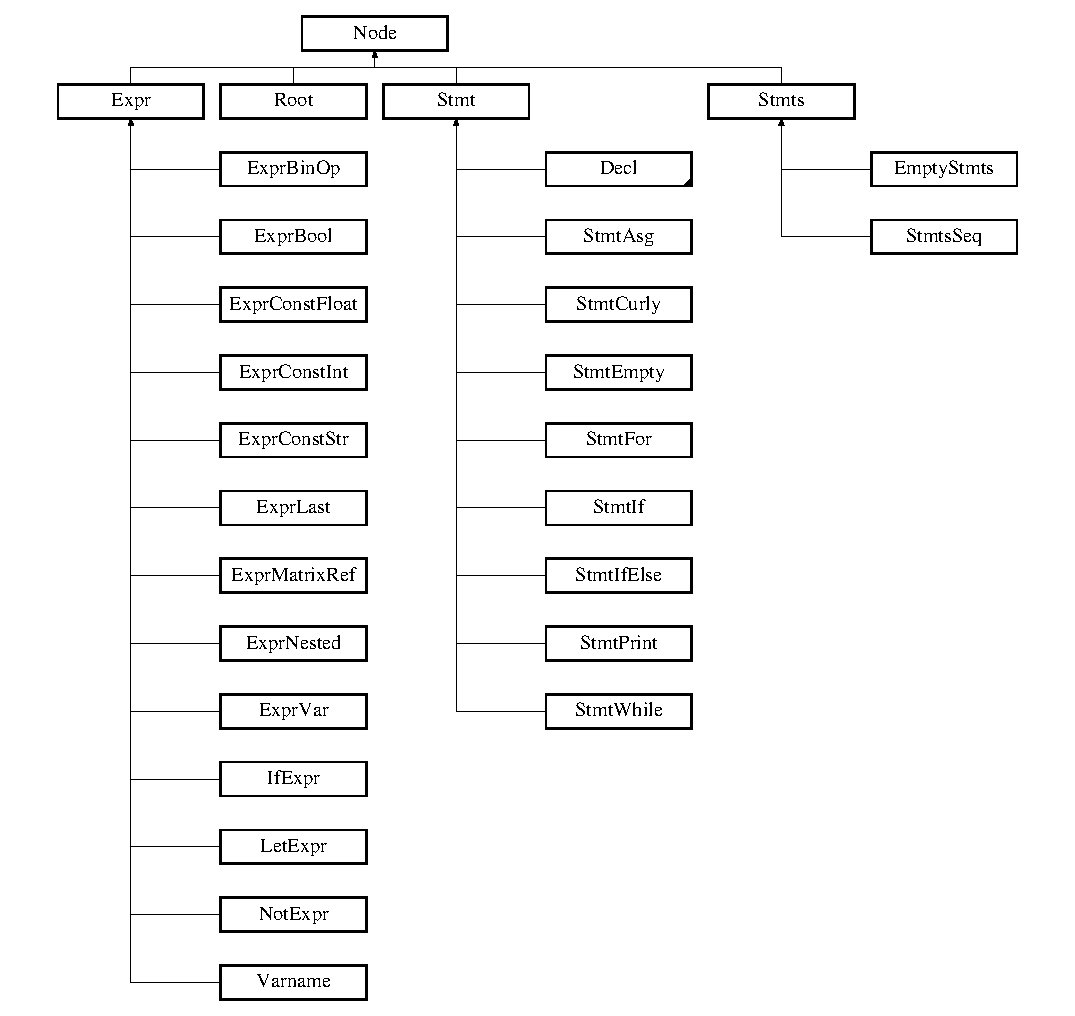
\includegraphics[height=12.000000cm]{classNode}
\end{center}
\end{figure}
\subsection*{Public Member Functions}
\begin{DoxyCompactItemize}
\item 
\hypertarget{classNode_a60ea533e0900961c05e701db70097136}{virtual std\-::string {\bfseries unparse} ()=0}\label{classNode_a60ea533e0900961c05e701db70097136}

\end{DoxyCompactItemize}


\subsection{Detailed Description}
\hyperlink{classNode}{Node} is the primary class from which all other classes inherit. Note that it is pure virtual, and thus cannot be instantiated 

The documentation for this class was generated from the following file\-:\begin{DoxyCompactItemize}
\item 
A\-S\-T.\-h\end{DoxyCompactItemize}

\hypertarget{classNotExpr}{\section{Not\-Expr Class Reference}
\label{classNotExpr}\index{Not\-Expr@{Not\-Expr}}
}


{\ttfamily \#include $<$A\-S\-T.\-h$>$}

Inheritance diagram for Not\-Expr\-:\begin{figure}[H]
\begin{center}
\leavevmode
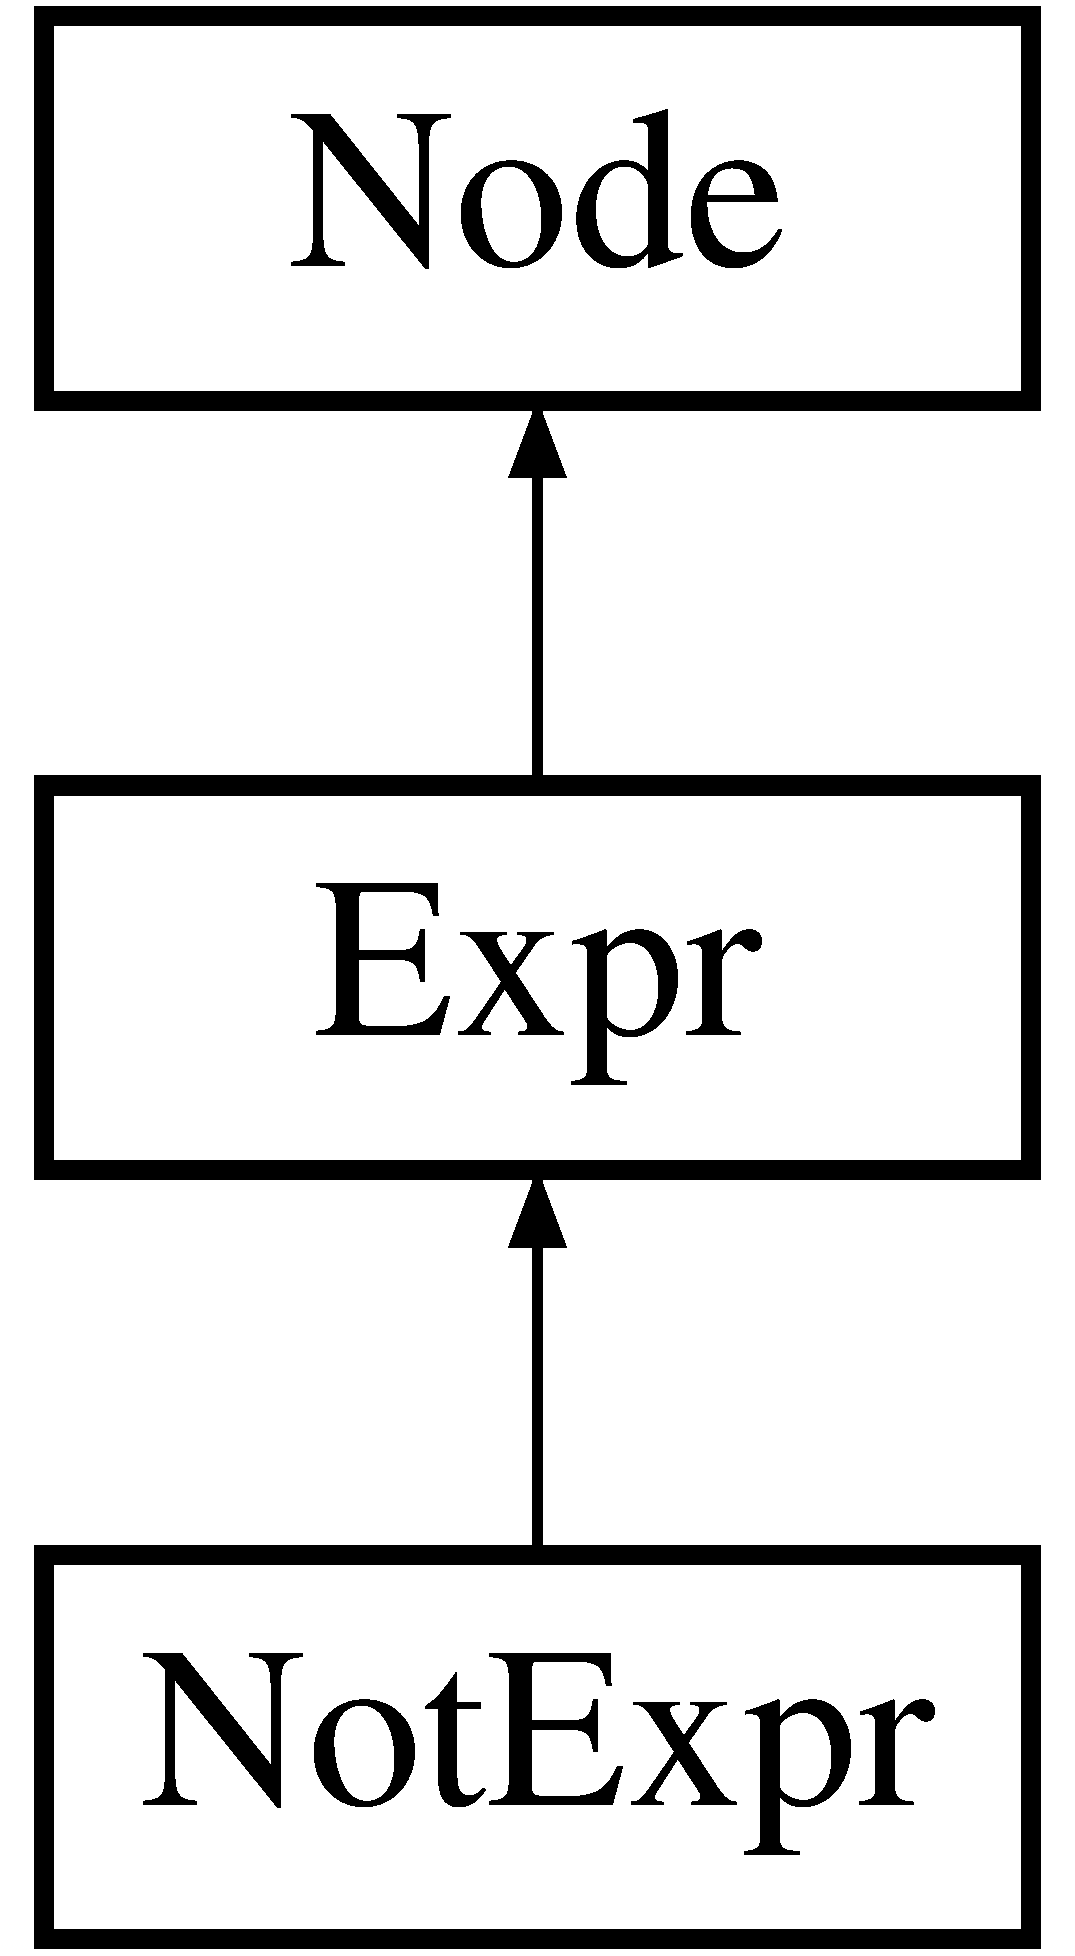
\includegraphics[height=3.000000cm]{classNotExpr}
\end{center}
\end{figure}
\subsection*{Public Member Functions}
\begin{DoxyCompactItemize}
\item 
\hypertarget{classNotExpr_a32d8529fc0f1e411b6a652a372202c7a}{{\bfseries Not\-Expr} (\hyperlink{classExpr}{Expr} $\ast$\-\_\-expr)}\label{classNotExpr_a32d8529fc0f1e411b6a652a372202c7a}

\item 
\hypertarget{classNotExpr_ab49f96d8f23e3fa6bb21376dc0fa5215}{std\-::string {\bfseries unparse} ()}\label{classNotExpr_ab49f96d8f23e3fa6bb21376dc0fa5215}

\end{DoxyCompactItemize}


\subsection{Detailed Description}
This class is for a 'not' expression 

The documentation for this class was generated from the following files\-:\begin{DoxyCompactItemize}
\item 
A\-S\-T.\-h\item 
A\-S\-T.\-cpp\end{DoxyCompactItemize}

\hypertarget{classNotOpToken}{\section{Not\-Op\-Token Class Reference}
\label{classNotOpToken}\index{Not\-Op\-Token@{Not\-Op\-Token}}
}
Inheritance diagram for Not\-Op\-Token\-:\begin{figure}[H]
\begin{center}
\leavevmode
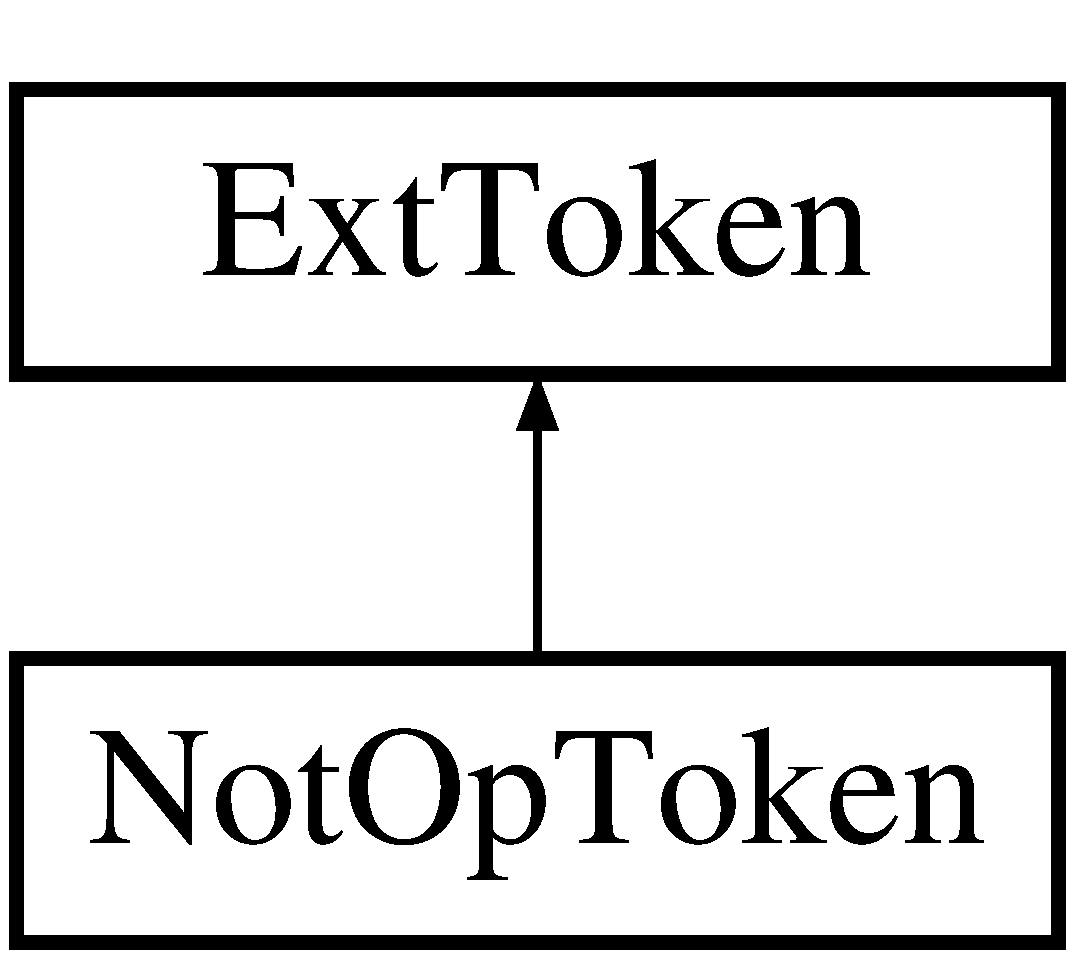
\includegraphics[height=2.000000cm]{classNotOpToken}
\end{center}
\end{figure}
\subsection*{Public Member Functions}
\begin{DoxyCompactItemize}
\item 
\hypertarget{classNotOpToken_afb8b9e96a178b1dfd69abf0a901dfddf}{{\bfseries Not\-Op\-Token} (\hyperlink{classParser}{Parser} $\ast$p, \hyperlink{classToken}{Token} $\ast$t)}\label{classNotOpToken_afb8b9e96a178b1dfd69abf0a901dfddf}

\item 
\hypertarget{classNotOpToken_a55a0dd53742aaca04338c16be079b031}{\hyperlink{classParseResult}{Parse\-Result} {\bfseries nud} ()}\label{classNotOpToken_a55a0dd53742aaca04338c16be079b031}

\item 
\hypertarget{classNotOpToken_a136a11f1e42542a9a58b7c14249c9d23}{std\-::string {\bfseries description} ()}\label{classNotOpToken_a136a11f1e42542a9a58b7c14249c9d23}

\end{DoxyCompactItemize}
\subsection*{Additional Inherited Members}


The documentation for this class was generated from the following file\-:\begin{DoxyCompactItemize}
\item 
ext\-Token.\-h\end{DoxyCompactItemize}

\hypertarget{classParser}{\section{Parser Class Reference}
\label{classParser}\index{Parser@{Parser}}
}
\subsection*{Public Member Functions}
\begin{DoxyCompactItemize}
\item 
\hyperlink{classParser_a12234f6cd36b61af4b50c94a179422c1}{Parser} ()
\item 
\hyperlink{classParseResult}{Parse\-Result} \hyperlink{classParser_a2c1a7aa0b09a43bc1eef460817efb1d6}{parse} (const char $\ast$text)
\item 
\hyperlink{classParseResult}{Parse\-Result} \hyperlink{classParser_a14e25c84322809e2f060dc530362ea71}{parse\-Program} ()
\item 
\hyperlink{classParseResult}{Parse\-Result} \hyperlink{classParser_ac646227983887c1cd13dae67fa1bc142}{parse\-Decl} ()
\item 
\hyperlink{classParseResult}{Parse\-Result} \hyperlink{classParser_a1e1f83c0f4b11148a356d951f191425e}{parse\-Standard\-Decl} ()
\item 
\hyperlink{classParseResult}{Parse\-Result} \hyperlink{classParser_a3a00df25fda2af308b69f05eed14ac69}{parse\-Matrix\-Decl} ()
\item 
\hypertarget{classParser_a452db3def31683cb0305e57a01489bd4}{\hyperlink{classParseResult}{Parse\-Result} {\bfseries parse\-Stmts} ()}\label{classParser_a452db3def31683cb0305e57a01489bd4}

\item 
\hyperlink{classParseResult}{Parse\-Result} \hyperlink{classParser_a9709c4793d0cce012d595f3ee416cd25}{parse\-Stmt} ()
\item 
\hypertarget{classParser_a50227dc24dc7a175ac0533d9957dfcf8}{\hyperlink{classParseResult}{Parse\-Result} {\bfseries parse\-Expr} (int rbp)}\label{classParser_a50227dc24dc7a175ac0533d9957dfcf8}

\item 
\hypertarget{classParser_ad40f1e5e4c66814f959d982f94b767a3}{\hyperlink{classParseResult}{Parse\-Result} {\bfseries parse\-True\-Kwd} ()}\label{classParser_ad40f1e5e4c66814f959d982f94b767a3}

\item 
\hypertarget{classParser_a56f03d2e70d12648c55ce56a11e63324}{\hyperlink{classParseResult}{Parse\-Result} {\bfseries parse\-False\-Kwd} ()}\label{classParser_a56f03d2e70d12648c55ce56a11e63324}

\item 
\hypertarget{classParser_a2b200b744e5bedf82ef6f610d7877cfc}{\hyperlink{classParseResult}{Parse\-Result} {\bfseries parse\-Int\-Const} ()}\label{classParser_a2b200b744e5bedf82ef6f610d7877cfc}

\item 
\hypertarget{classParser_aaf7b1176fd53246f59577c7eec8b9d22}{\hyperlink{classParseResult}{Parse\-Result} {\bfseries parse\-Float\-Const} ()}\label{classParser_aaf7b1176fd53246f59577c7eec8b9d22}

\item 
\hypertarget{classParser_a4d8930d45c2b730912154c46cc54833c}{\hyperlink{classParseResult}{Parse\-Result} {\bfseries parse\-String\-Const} ()}\label{classParser_a4d8930d45c2b730912154c46cc54833c}

\item 
\hypertarget{classParser_a49c9b3d31ca060c97873e5485d518da3}{\hyperlink{classParseResult}{Parse\-Result} {\bfseries parse\-Char\-Const} ()}\label{classParser_a49c9b3d31ca060c97873e5485d518da3}

\item 
\hypertarget{classParser_a8c1baf62f71da64590e883e51ce622ca}{\hyperlink{classParseResult}{Parse\-Result} {\bfseries parse\-Variable\-Name} ()}\label{classParser_a8c1baf62f71da64590e883e51ce622ca}

\item 
\hypertarget{classParser_aec4c38e1e63c9becfd3a8fc4a1a73f01}{\hyperlink{classParseResult}{Parse\-Result} {\bfseries parse\-Nested\-Expr} ()}\label{classParser_aec4c38e1e63c9becfd3a8fc4a1a73f01}

\item 
\hypertarget{classParser_a1503ceff46112d6d4f0e01b5fb77afcd}{\hyperlink{classParseResult}{Parse\-Result} {\bfseries parse\-Not\-Expr} ()}\label{classParser_a1503ceff46112d6d4f0e01b5fb77afcd}

\item 
\hypertarget{classParser_aa24c33b04779801b330d7fe5a74349e5}{\hyperlink{classParseResult}{Parse\-Result} {\bfseries parse\-Let\-Expr} ()}\label{classParser_aa24c33b04779801b330d7fe5a74349e5}

\item 
\hypertarget{classParser_a555bc6f671d408208e6d049f8e9f3c86}{\hyperlink{classParseResult}{Parse\-Result} {\bfseries parse\-If\-Expr} ()}\label{classParser_a555bc6f671d408208e6d049f8e9f3c86}

\item 
\hypertarget{classParser_ae09cb2b5a7f80c6ad4ad9ccf27a746ca}{\hyperlink{classParseResult}{Parse\-Result} {\bfseries parse\-Addition} (\hyperlink{classParseResult}{Parse\-Result} left)}\label{classParser_ae09cb2b5a7f80c6ad4ad9ccf27a746ca}

\item 
\hypertarget{classParser_a52e6a57d53fc98e5819cc51b3cbe5bd5}{\hyperlink{classParseResult}{Parse\-Result} {\bfseries parse\-Multiplication} (\hyperlink{classParseResult}{Parse\-Result} left)}\label{classParser_a52e6a57d53fc98e5819cc51b3cbe5bd5}

\item 
\hypertarget{classParser_ac22cf1f77e0ca4c23942d5cbcc47eb37}{\hyperlink{classParseResult}{Parse\-Result} {\bfseries parse\-Subtraction} (\hyperlink{classParseResult}{Parse\-Result} left)}\label{classParser_ac22cf1f77e0ca4c23942d5cbcc47eb37}

\item 
\hypertarget{classParser_ad05e6cd1bf83179ecb727b83cbbd0c4e}{\hyperlink{classParseResult}{Parse\-Result} {\bfseries parse\-Division} (\hyperlink{classParseResult}{Parse\-Result} left)}\label{classParser_ad05e6cd1bf83179ecb727b83cbbd0c4e}

\item 
\hypertarget{classParser_ab42ecabc4dbe601d5ed9667351c0c0b8}{\hyperlink{classParseResult}{Parse\-Result} {\bfseries parse\-Relational\-Expr} (\hyperlink{classParseResult}{Parse\-Result} left)}\label{classParser_ab42ecabc4dbe601d5ed9667351c0c0b8}

\item 
\hypertarget{classParser_a3199aab5275c8b6477245eb866fabf35}{void {\bfseries match} (token\-Type tt)}\label{classParser_a3199aab5275c8b6477245eb866fabf35}

\item 
\hypertarget{classParser_a151ffb920a67527813d77bc4ba44c4a7}{bool {\bfseries attempt\-Match} (token\-Type tt)}\label{classParser_a151ffb920a67527813d77bc4ba44c4a7}

\item 
\hypertarget{classParser_a67a10b685bd263477b5f59f1923cdec3}{bool {\bfseries next\-Is} (token\-Type tt)}\label{classParser_a67a10b685bd263477b5f59f1923cdec3}

\item 
\hypertarget{classParser_a324a5bb61c9dfc645300a92aecd6fe69}{void {\bfseries next\-Token} ()}\label{classParser_a324a5bb61c9dfc645300a92aecd6fe69}

\item 
\hypertarget{classParser_af65b651dfccdd3644c27ec5ae3e82b9d}{std\-::string {\bfseries terminal\-Description} (token\-Type terminal)}\label{classParser_af65b651dfccdd3644c27ec5ae3e82b9d}

\item 
\hypertarget{classParser_a72a0ed0baf243132fc4656c89bddc852}{std\-::string {\bfseries make\-Error\-Msg} (token\-Type terminal)}\label{classParser_a72a0ed0baf243132fc4656c89bddc852}

\item 
\hypertarget{classParser_a4daf7772e349c22a3eb942021a242167}{std\-::string {\bfseries make\-Error\-Msg\-Expected} (token\-Type terminal)}\label{classParser_a4daf7772e349c22a3eb942021a242167}

\item 
\hypertarget{classParser_a17cffdf7846dd5506546b7f9d83d4d36}{std\-::string {\bfseries make\-Error\-Msg} (const char $\ast$msg)}\label{classParser_a17cffdf7846dd5506546b7f9d83d4d36}

\end{DoxyCompactItemize}
\subsection*{Public Attributes}
\begin{DoxyCompactItemize}
\item 
\hypertarget{classParser_a3606ff327be18af7f76df95f50851633}{\hyperlink{classExtToken}{Ext\-Token} $\ast$ {\bfseries tokens}}\label{classParser_a3606ff327be18af7f76df95f50851633}

\item 
\hypertarget{classParser_a75ab2e2b9385c14e5f967f873340ed11}{\hyperlink{classExtToken}{Ext\-Token} $\ast$ {\bfseries curr\-Token}}\label{classParser_a75ab2e2b9385c14e5f967f873340ed11}

\item 
\hypertarget{classParser_a4bcf7560a5ea1b486bbe4bb54a5a22eb}{\hyperlink{classExtToken}{Ext\-Token} $\ast$ {\bfseries prev\-Token}}\label{classParser_a4bcf7560a5ea1b486bbe4bb54a5a22eb}

\item 
\hypertarget{classParser_a0910de176dcc1cdfbf7ad99622ce9dd5}{\hyperlink{classToken}{Token} $\ast$ {\bfseries stokens}}\label{classParser_a0910de176dcc1cdfbf7ad99622ce9dd5}

\item 
\hypertarget{classParser_ab2ef99ea9e732f5fd176b3949a6c32af}{\hyperlink{classScanner}{Scanner} $\ast$ {\bfseries s}}\label{classParser_ab2ef99ea9e732f5fd176b3949a6c32af}

\end{DoxyCompactItemize}


\subsection{Constructor \& Destructor Documentation}
\hypertarget{classParser_a12234f6cd36b61af4b50c94a179422c1}{\index{Parser@{Parser}!Parser@{Parser}}
\index{Parser@{Parser}!Parser@{Parser}}
\subsubsection[{Parser}]{\setlength{\rightskip}{0pt plus 5cm}Parser\-::\-Parser (
\begin{DoxyParamCaption}
{}
\end{DoxyParamCaption}
)}}\label{classParser_a12234f6cd36b61af4b50c94a179422c1}
This is the constructor for the parser, it sets up the members that we need to parse the program. In this case, it really may as well be the default constructor with an empty body 

\subsection{Member Function Documentation}
\hypertarget{classParser_a2c1a7aa0b09a43bc1eef460817efb1d6}{\index{Parser@{Parser}!parse@{parse}}
\index{parse@{parse}!Parser@{Parser}}
\subsubsection[{parse}]{\setlength{\rightskip}{0pt plus 5cm}{\bf Parse\-Result} Parser\-::parse (
\begin{DoxyParamCaption}
\item[{const char $\ast$}]{text}
\end{DoxyParamCaption}
)}}\label{classParser_a2c1a7aa0b09a43bc1eef460817efb1d6}
\hyperlink{classParser}{Parser} obtains the necessary data, by setting up the scanner, extending the token list, etc. \hypertarget{classParser_ac646227983887c1cd13dae67fa1bc142}{\index{Parser@{Parser}!parse\-Decl@{parse\-Decl}}
\index{parse\-Decl@{parse\-Decl}!Parser@{Parser}}
\subsubsection[{parse\-Decl}]{\setlength{\rightskip}{0pt plus 5cm}{\bf Parse\-Result} Parser\-::parse\-Decl (
\begin{DoxyParamCaption}
{}
\end{DoxyParamCaption}
)}}\label{classParser_ac646227983887c1cd13dae67fa1bc142}
parse\-Decl is the general declaration, figures out if it should use standard or matrix decl parsing \hyperlink{classDecl}{Decl} \-:\-: Matrix variable\-Name ....

\hyperlink{classDecl}{Decl} \-:\-:= Type variable\-Name semi\-Colon \hypertarget{classParser_a3a00df25fda2af308b69f05eed14ac69}{\index{Parser@{Parser}!parse\-Matrix\-Decl@{parse\-Matrix\-Decl}}
\index{parse\-Matrix\-Decl@{parse\-Matrix\-Decl}!Parser@{Parser}}
\subsubsection[{parse\-Matrix\-Decl}]{\setlength{\rightskip}{0pt plus 5cm}{\bf Parse\-Result} Parser\-::parse\-Matrix\-Decl (
\begin{DoxyParamCaption}
{}
\end{DoxyParamCaption}
)}}\label{classParser_a3a00df25fda2af308b69f05eed14ac69}
Matrix\-Decl identical purpose of parse\-Decl, handles special matrix syntax. \hyperlink{classDecl}{Decl} \-:\-:= 'Matrix' var\-Name '\mbox{[}' \hyperlink{classExpr}{Expr} ',' \hyperlink{classExpr}{Expr} '\mbox{]}' var\-Name ',' var\-Name '=' \hyperlink{classExpr}{Expr} ';'

\hyperlink{classDecl}{Decl} \-:\-:= 'Matrix' var\-Name '=' \hyperlink{classExpr}{Expr} ';' \hypertarget{classParser_a14e25c84322809e2f060dc530362ea71}{\index{Parser@{Parser}!parse\-Program@{parse\-Program}}
\index{parse\-Program@{parse\-Program}!Parser@{Parser}}
\subsubsection[{parse\-Program}]{\setlength{\rightskip}{0pt plus 5cm}{\bf Parse\-Result} Parser\-::parse\-Program (
\begin{DoxyParamCaption}
{}
\end{DoxyParamCaption}
)}}\label{classParser_a14e25c84322809e2f060dc530362ea71}
parse\-Program parses the root of the program, i.\-e main()\{statements\}, separating the main method from statements inside. Program \-:\-:= var\-Name '(' ')' '\{' \hyperlink{classStmts}{Stmts} '\}' \hypertarget{classParser_a1e1f83c0f4b11148a356d951f191425e}{\index{Parser@{Parser}!parse\-Standard\-Decl@{parse\-Standard\-Decl}}
\index{parse\-Standard\-Decl@{parse\-Standard\-Decl}!Parser@{Parser}}
\subsubsection[{parse\-Standard\-Decl}]{\setlength{\rightskip}{0pt plus 5cm}{\bf Parse\-Result} Parser\-::parse\-Standard\-Decl (
\begin{DoxyParamCaption}
{}
\end{DoxyParamCaption}
)}}\label{classParser_a1e1f83c0f4b11148a356d951f191425e}
This function parse standard\-Decl parses the nonmatrix declarations \hyperlink{classDecl}{Decl} \-:\-:= integer\-Kwd var\-Name $\vert$ float\-Kwd var\-Name $\vert$ string\-Kwd var\-Name Type \-:\-:= int\-Kwd

Type \-:\-:= float\-Kwd

Type \-:\-:= string\-Kwd

Type \-:\-:= bool\-Kwd \hypertarget{classParser_a9709c4793d0cce012d595f3ee416cd25}{\index{Parser@{Parser}!parse\-Stmt@{parse\-Stmt}}
\index{parse\-Stmt@{parse\-Stmt}!Parser@{Parser}}
\subsubsection[{parse\-Stmt}]{\setlength{\rightskip}{0pt plus 5cm}{\bf Parse\-Result} Parser\-::parse\-Stmt (
\begin{DoxyParamCaption}
{}
\end{DoxyParamCaption}
)}}\label{classParser_a9709c4793d0cce012d595f3ee416cd25}
\hyperlink{classStmt}{Stmt} general case is handled here and handed off to each specific parser function base on type \hyperlink{classStmt}{Stmt} \-:\-:= \hyperlink{classDecl}{Decl} 

The documentation for this class was generated from the following files\-:\begin{DoxyCompactItemize}
\item 
parser.\-h\item 
parser.\-cpp\end{DoxyCompactItemize}

\hypertarget{classParseResult}{\section{Parse\-Result Class Reference}
\label{classParseResult}\index{Parse\-Result@{Parse\-Result}}
}
\subsection*{Public Attributes}
\begin{DoxyCompactItemize}
\item 
\hypertarget{classParseResult_ab2dd8deb95c5177148f488ca5d31307a}{std\-::string {\bfseries errors}}\label{classParseResult_ab2dd8deb95c5177148f488ca5d31307a}

\item 
\hypertarget{classParseResult_aa04c6ed3cba109f276e5bc089ca2ff15}{\hyperlink{classNode}{Node} $\ast$ {\bfseries ast}}\label{classParseResult_aa04c6ed3cba109f276e5bc089ca2ff15}

\item 
\hypertarget{classParseResult_a64eb6658c1fc5bbf35fdce181f6845d5}{bool {\bfseries ok}}\label{classParseResult_a64eb6658c1fc5bbf35fdce181f6845d5}

\end{DoxyCompactItemize}


The documentation for this class was generated from the following files\-:\begin{DoxyCompactItemize}
\item 
parse\-Result.\-h\item 
parse\-Result.\-cpp\end{DoxyCompactItemize}

\hypertarget{classParserTestSuite}{\section{Parser\-Test\-Suite Class Reference}
\label{classParserTestSuite}\index{Parser\-Test\-Suite@{Parser\-Test\-Suite}}
}
Inheritance diagram for Parser\-Test\-Suite\-:\begin{figure}[H]
\begin{center}
\leavevmode
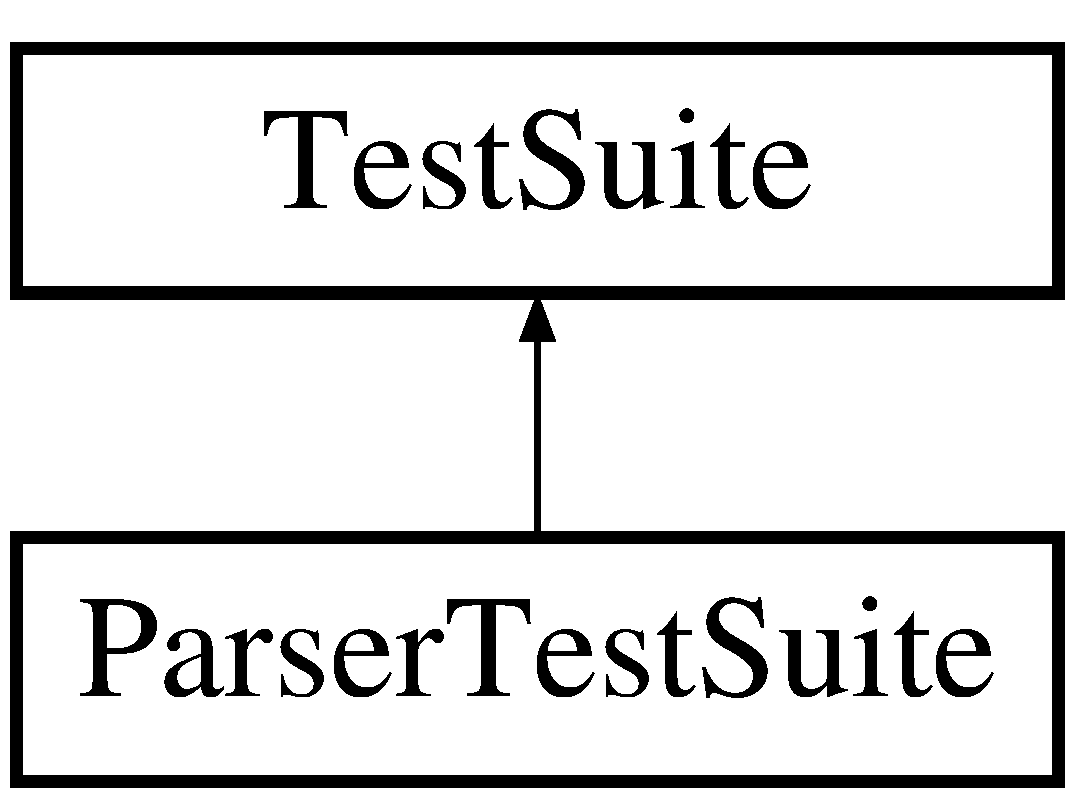
\includegraphics[height=2.000000cm]{classParserTestSuite}
\end{center}
\end{figure}
\subsection*{Public Member Functions}
\begin{DoxyCompactItemize}
\item 
\hypertarget{classParserTestSuite_ab7eff3217b5e28c9003f27c51da107ac}{void {\bfseries test\-\_\-setup\-\_\-code} ()}\label{classParserTestSuite_ab7eff3217b5e28c9003f27c51da107ac}

\item 
\hypertarget{classParserTestSuite_ac4a829a66a1582bee38e90ac3f0355f4}{void {\bfseries test\-\_\-parse\-\_\-bad\-\_\-syntax} ()}\label{classParserTestSuite_ac4a829a66a1582bee38e90ac3f0355f4}

\item 
\hypertarget{classParserTestSuite_a26eed485bc2671f4ac256ef97a21b704}{void {\bfseries test\-\_\-parse\-\_\-sample\-\_\-1} ()}\label{classParserTestSuite_a26eed485bc2671f4ac256ef97a21b704}

\item 
\hypertarget{classParserTestSuite_a0f1d6af1e07e35541fb83416d5e3e229}{void {\bfseries test\-\_\-parse\-\_\-sample\-\_\-2} ()}\label{classParserTestSuite_a0f1d6af1e07e35541fb83416d5e3e229}

\item 
\hypertarget{classParserTestSuite_aecc132f6b6dbb2e5bba08baec64f3f65}{void {\bfseries test\-\_\-parse\-\_\-sample\-\_\-3} ()}\label{classParserTestSuite_aecc132f6b6dbb2e5bba08baec64f3f65}

\item 
\hypertarget{classParserTestSuite_a6e5dfaf7b8ddc98001a4fec39b3f0a79}{void {\bfseries test\-\_\-parse\-\_\-sample\-\_\-4} ()}\label{classParserTestSuite_a6e5dfaf7b8ddc98001a4fec39b3f0a79}

\item 
\hypertarget{classParserTestSuite_a5b9a3cf2b76271244baaaaa4c8b7f7d5}{void {\bfseries test\-\_\-parse\-\_\-sample\-\_\-5} ()}\label{classParserTestSuite_a5b9a3cf2b76271244baaaaa4c8b7f7d5}

\item 
\hypertarget{classParserTestSuite_ae59d0f6d92f8d83833d51ef01479fdeb}{void {\bfseries test\-\_\-parse\-\_\-mysample} ()}\label{classParserTestSuite_ae59d0f6d92f8d83833d51ef01479fdeb}

\item 
\hypertarget{classParserTestSuite_a379db1a22b2c32defb8395b9b2166f76}{void {\bfseries test\-\_\-parse\-\_\-forest\-Loss\-V2} ()}\label{classParserTestSuite_a379db1a22b2c32defb8395b9b2166f76}

\end{DoxyCompactItemize}
\subsection*{Public Attributes}
\begin{DoxyCompactItemize}
\item 
\hypertarget{classParserTestSuite_a0c4943b3d23b79be363ba9e1ac7c02ed}{\hyperlink{classScanner}{Scanner} $\ast$ {\bfseries s}}\label{classParserTestSuite_a0c4943b3d23b79be363ba9e1ac7c02ed}

\item 
\hypertarget{classParserTestSuite_a1d637f2f8be1326423ee5b4fd270c553}{\hyperlink{classParser}{Parser} $\ast$ {\bfseries p}}\label{classParserTestSuite_a1d637f2f8be1326423ee5b4fd270c553}

\end{DoxyCompactItemize}


The documentation for this class was generated from the following file\-:\begin{DoxyCompactItemize}
\item 
parser\-\_\-tests.\-h\end{DoxyCompactItemize}

\hypertarget{classPlusSignToken}{\section{Plus\-Sign\-Token Class Reference}
\label{classPlusSignToken}\index{Plus\-Sign\-Token@{Plus\-Sign\-Token}}
}
Inheritance diagram for Plus\-Sign\-Token\-:\begin{figure}[H]
\begin{center}
\leavevmode
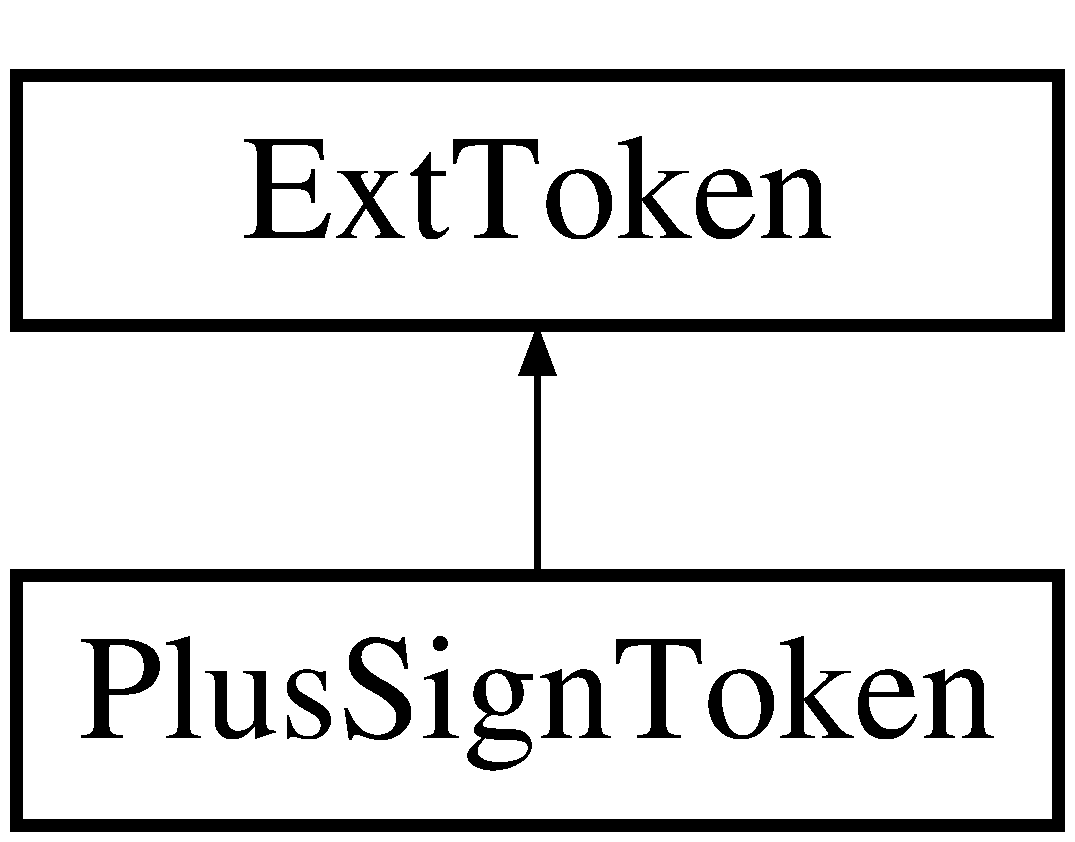
\includegraphics[height=2.000000cm]{classPlusSignToken}
\end{center}
\end{figure}
\subsection*{Public Member Functions}
\begin{DoxyCompactItemize}
\item 
\hypertarget{classPlusSignToken_ad480457c426f911f8286a73e8cf7f949}{{\bfseries Plus\-Sign\-Token} (\hyperlink{classParser}{Parser} $\ast$p, \hyperlink{classToken}{Token} $\ast$t)}\label{classPlusSignToken_ad480457c426f911f8286a73e8cf7f949}

\item 
\hypertarget{classPlusSignToken_a4d79a17891f92800259308ce71402526}{\hyperlink{classParseResult}{Parse\-Result} {\bfseries led} (\hyperlink{classParseResult}{Parse\-Result} left)}\label{classPlusSignToken_a4d79a17891f92800259308ce71402526}

\item 
\hypertarget{classPlusSignToken_a61a05ac9660848e13da97d5746808868}{std\-::string {\bfseries description} ()}\label{classPlusSignToken_a61a05ac9660848e13da97d5746808868}

\item 
\hypertarget{classPlusSignToken_a80753eec970928e042da350df83150f2}{int {\bfseries lbp} ()}\label{classPlusSignToken_a80753eec970928e042da350df83150f2}

\end{DoxyCompactItemize}
\subsection*{Additional Inherited Members}


The documentation for this class was generated from the following file\-:\begin{DoxyCompactItemize}
\item 
ext\-Token.\-h\end{DoxyCompactItemize}

\hypertarget{classRegexTestSuite}{\section{Regex\-Test\-Suite Class Reference}
\label{classRegexTestSuite}\index{Regex\-Test\-Suite@{Regex\-Test\-Suite}}
}
Inheritance diagram for Regex\-Test\-Suite\-:\begin{figure}[H]
\begin{center}
\leavevmode
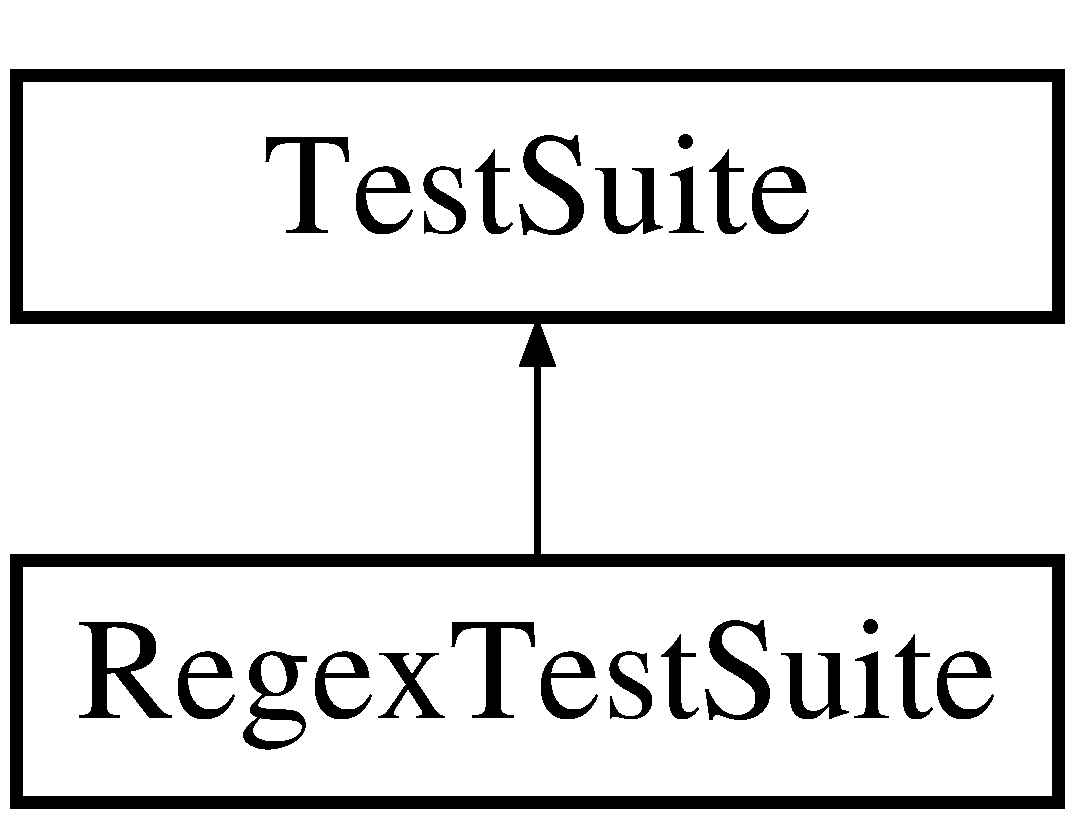
\includegraphics[height=2.000000cm]{classRegexTestSuite}
\end{center}
\end{figure}
\subsection*{Public Member Functions}
\begin{DoxyCompactItemize}
\item 
\hypertarget{classRegexTestSuite_aac0838d917fd9fd6cc71ee086c644555}{void {\bfseries test\-\_\-make\-\_\-match\-Regex\-\_\-match} (void)}\label{classRegexTestSuite_aac0838d917fd9fd6cc71ee086c644555}

\item 
\hypertarget{classRegexTestSuite_ad9c02b9f4fd7feca750d476cda8e0c60}{void {\bfseries test\-\_\-make\-\_\-match\-Regex\-\_\-no\-\_\-match} (void)}\label{classRegexTestSuite_ad9c02b9f4fd7feca750d476cda8e0c60}

\item 
\hypertarget{classRegexTestSuite_a0f46b90e2c0a1c98750a3335d086979a}{void {\bfseries test\-\_\-make\-\_\-match\-Regex\-\_\-match\-\_\-string\-\_\-copy} (void)}\label{classRegexTestSuite_a0f46b90e2c0a1c98750a3335d086979a}

\end{DoxyCompactItemize}


The documentation for this class was generated from the following file\-:\begin{DoxyCompactItemize}
\item 
regex\-\_\-tests.\-h\end{DoxyCompactItemize}

\hypertarget{classRelationalOpToken}{\section{Relational\-Op\-Token Class Reference}
\label{classRelationalOpToken}\index{Relational\-Op\-Token@{Relational\-Op\-Token}}
}
Inheritance diagram for Relational\-Op\-Token\-:\begin{figure}[H]
\begin{center}
\leavevmode
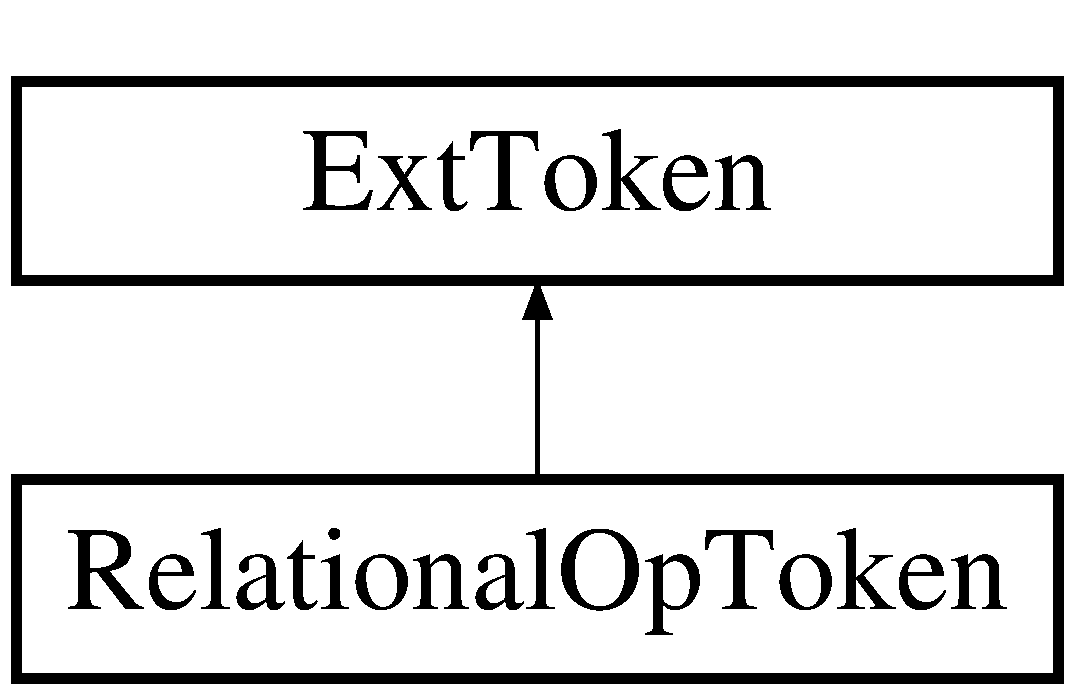
\includegraphics[height=2.000000cm]{classRelationalOpToken}
\end{center}
\end{figure}
\subsection*{Public Member Functions}
\begin{DoxyCompactItemize}
\item 
\hypertarget{classRelationalOpToken_a1ede45cf178138ff12beba209681be51}{{\bfseries Relational\-Op\-Token} (\hyperlink{classParser}{Parser} $\ast$p, \hyperlink{classToken}{Token} $\ast$t, std\-::string d)}\label{classRelationalOpToken_a1ede45cf178138ff12beba209681be51}

\item 
\hypertarget{classRelationalOpToken_a426c64391e7b3272d8e6277964730e05}{\hyperlink{classParseResult}{Parse\-Result} {\bfseries led} (\hyperlink{classParseResult}{Parse\-Result} left)}\label{classRelationalOpToken_a426c64391e7b3272d8e6277964730e05}

\item 
\hypertarget{classRelationalOpToken_ada096491d9553aea21089230489d6aef}{int {\bfseries lbp} ()}\label{classRelationalOpToken_ada096491d9553aea21089230489d6aef}

\end{DoxyCompactItemize}
\subsection*{Additional Inherited Members}


The documentation for this class was generated from the following file\-:\begin{DoxyCompactItemize}
\item 
ext\-Token.\-h\end{DoxyCompactItemize}

\hypertarget{classRoot}{\section{Root Class Reference}
\label{classRoot}\index{Root@{Root}}
}


{\ttfamily \#include $<$A\-S\-T.\-h$>$}

Inheritance diagram for Root\-:\begin{figure}[H]
\begin{center}
\leavevmode
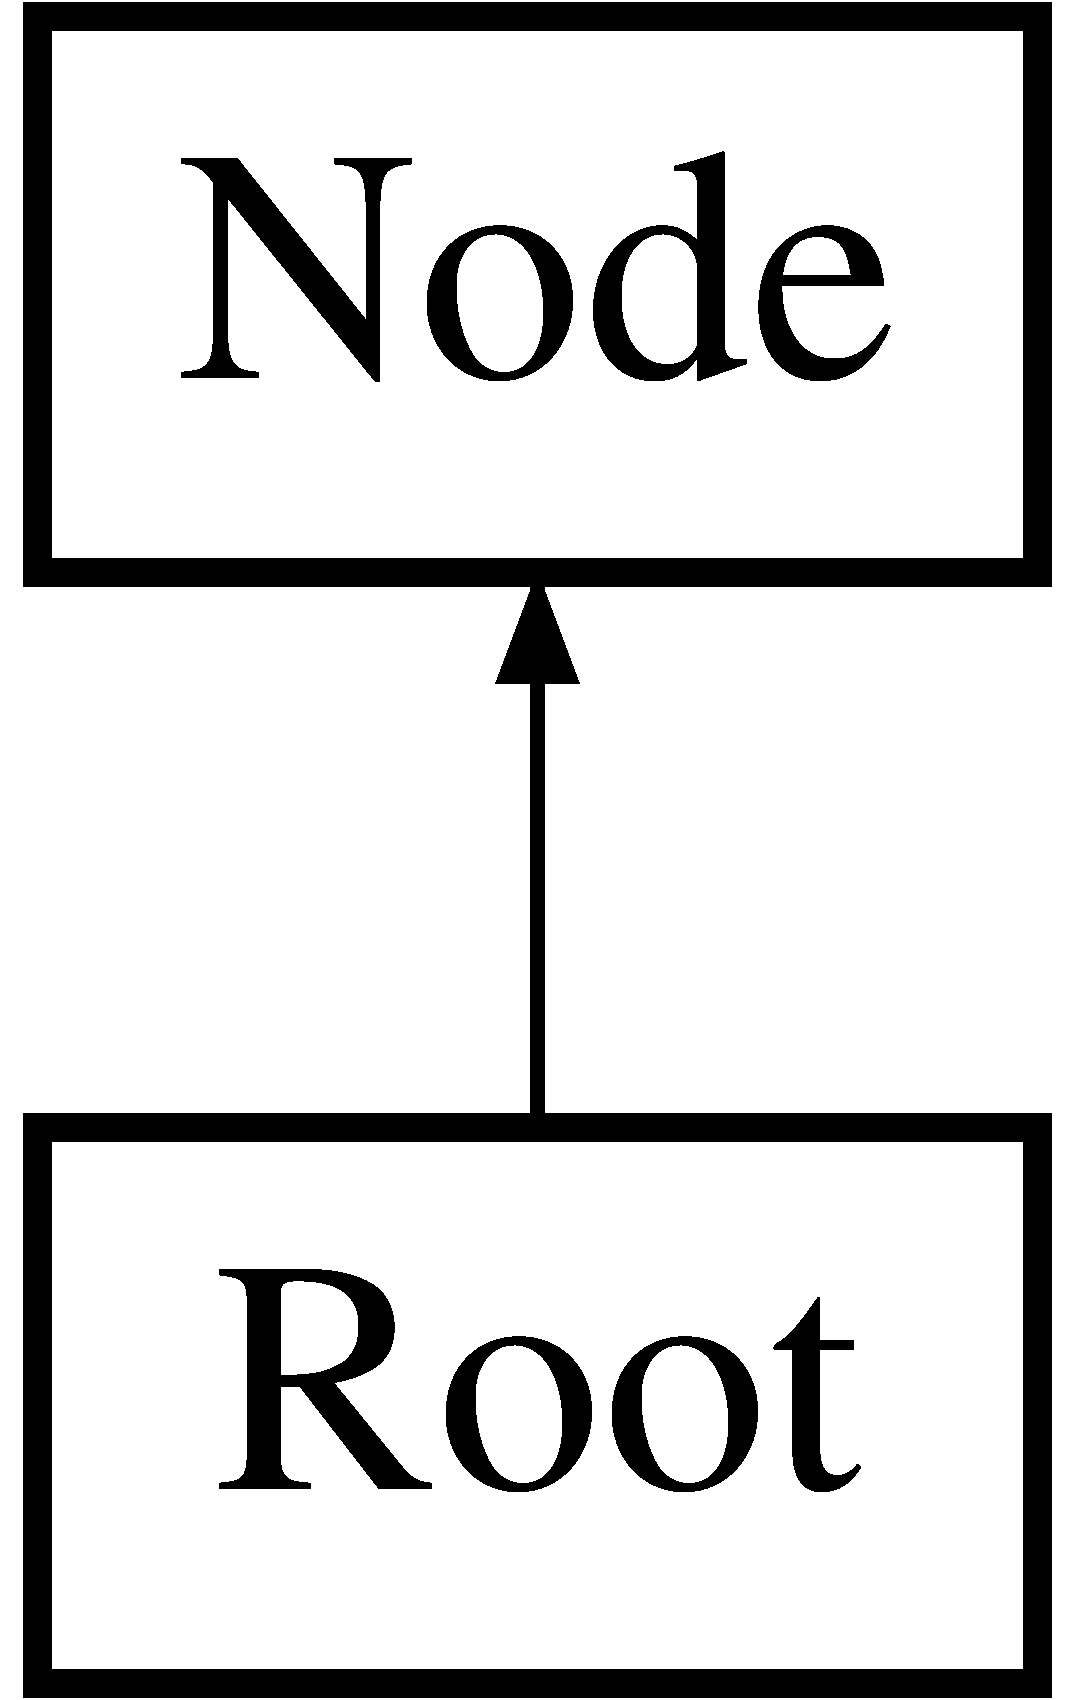
\includegraphics[height=2.000000cm]{classRoot}
\end{center}
\end{figure}
\subsection*{Public Member Functions}
\begin{DoxyCompactItemize}
\item 
\hyperlink{classRoot_a1041d19e10fd8219cb29664831fae8cf}{Root} (\hyperlink{classVarname}{Varname} $\ast$v, \hyperlink{classStmts}{Stmts} $\ast$s)
\item 
std\-::string \hyperlink{classRoot_a3fd0b715e1f0dfa2bb6b40b03f85c982}{unparse} ()
\end{DoxyCompactItemize}


\subsection{Detailed Description}
\hyperlink{classRoot}{Root} puts the first line in the program, \char`\"{}main()\{stmts\}\char`\"{} into the syntax tree 

\subsection{Constructor \& Destructor Documentation}
\hypertarget{classRoot_a1041d19e10fd8219cb29664831fae8cf}{\index{Root@{Root}!Root@{Root}}
\index{Root@{Root}!Root@{Root}}
\subsubsection[{Root}]{\setlength{\rightskip}{0pt plus 5cm}Root\-::\-Root (
\begin{DoxyParamCaption}
\item[{{\bf Varname} $\ast$}]{v, }
\item[{{\bf Stmts} $\ast$}]{s}
\end{DoxyParamCaption}
)\hspace{0.3cm}{\ttfamily [inline]}}}\label{classRoot_a1041d19e10fd8219cb29664831fae8cf}
This constructor takes the main function name, and the statements in the F\-C\-A\-L program as its param 
\begin{DoxyParams}{Parameters}
{\em $\ast$v} & the varname in the first function of the program, i.\-e main \\
\hline
{\em $\ast$s} & the sequence of stmts objects which compose the F\-C\-A\-L program \\
\hline
\end{DoxyParams}


\subsection{Member Function Documentation}
\hypertarget{classRoot_a3fd0b715e1f0dfa2bb6b40b03f85c982}{\index{Root@{Root}!unparse@{unparse}}
\index{unparse@{unparse}!Root@{Root}}
\subsubsection[{unparse}]{\setlength{\rightskip}{0pt plus 5cm}std\-::string Root\-::unparse (
\begin{DoxyParamCaption}
{}
\end{DoxyParamCaption}
)\hspace{0.3cm}{\ttfamily [virtual]}}}\label{classRoot_a3fd0b715e1f0dfa2bb6b40b03f85c982}
We have an unparse string that returns the F\-C\-A\-L string after being parsed, this unparse string is implemented in almost every class 

Implements \hyperlink{classNode}{Node}.



The documentation for this class was generated from the following files\-:\begin{DoxyCompactItemize}
\item 
A\-S\-T.\-h\item 
A\-S\-T.\-cpp\end{DoxyCompactItemize}

\hypertarget{classScanner}{\section{Scanner Class Reference}
\label{classScanner}\index{Scanner@{Scanner}}
}
\subsection*{Public Member Functions}
\begin{DoxyCompactItemize}
\item 
\hypertarget{classScanner_a4cf90c9e68bfb17f23af7368ff15766e}{\hyperlink{classToken}{Token} $\ast$ {\bfseries scan} (const char $\ast$)}\label{classScanner_a4cf90c9e68bfb17f23af7368ff15766e}

\end{DoxyCompactItemize}
\subsection*{Public Attributes}
\begin{DoxyCompactItemize}
\item 
\hypertarget{classScanner_abff69d92b8f5d9112d5af0d106fd42ed}{regex\-\_\-t $\ast$$\ast$ {\bfseries type\-Database}}\label{classScanner_abff69d92b8f5d9112d5af0d106fd42ed}

\end{DoxyCompactItemize}


The documentation for this class was generated from the following files\-:\begin{DoxyCompactItemize}
\item 
scanner.\-h\item 
scanner.\-cpp\end{DoxyCompactItemize}

\hypertarget{classScannerTestSuite}{\section{Scanner\-Test\-Suite Class Reference}
\label{classScannerTestSuite}\index{Scanner\-Test\-Suite@{Scanner\-Test\-Suite}}
}
Inheritance diagram for Scanner\-Test\-Suite\-:\begin{figure}[H]
\begin{center}
\leavevmode
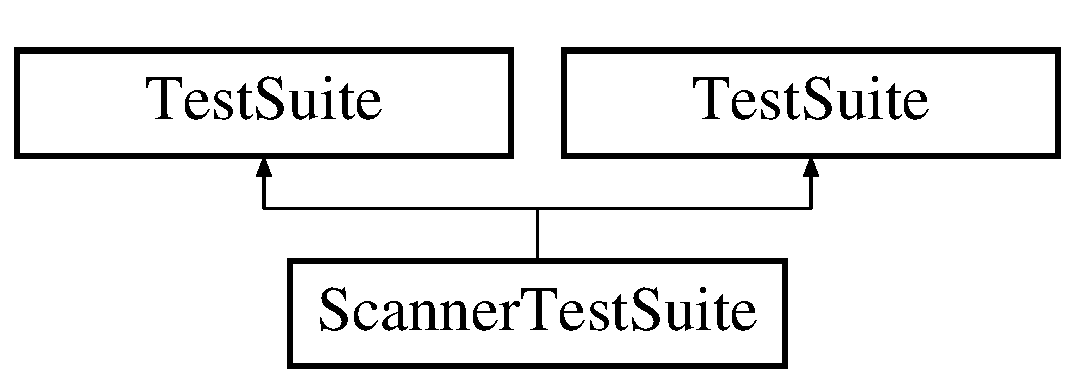
\includegraphics[height=2.000000cm]{classScannerTestSuite}
\end{center}
\end{figure}
\subsection*{Public Member Functions}
\begin{DoxyCompactItemize}
\item 
\hypertarget{classScannerTestSuite_a741342209e22b68988214db2c468a556}{char $\ast$$\ast$ {\bfseries make\-Args} (const char $\ast$a0, const char $\ast$a1)}\label{classScannerTestSuite_a741342209e22b68988214db2c468a556}

\item 
\hypertarget{classScannerTestSuite_ad123ba96fb82266232b05190c14ee65f}{void {\bfseries write\-File} (const string text, const string filename)}\label{classScannerTestSuite_ad123ba96fb82266232b05190c14ee65f}

\item 
\hypertarget{classScannerTestSuite_a5633fb2c0b238cf6a9f03ffa4c6f4257}{char $\ast$ {\bfseries read\-File} (const char $\ast$fn)}\label{classScannerTestSuite_a5633fb2c0b238cf6a9f03ffa4c6f4257}

\item 
void \hyperlink{classScannerTestSuite_a7c1f696a90f5d8f22d6af01daffa4077}{unparse\-\_\-tests} (string file)
\item 
void \hyperlink{classScannerTestSuite_a56fe193039ed980337d33d3a75909f1c}{test\-\_\-sample\-\_\-1} (void)
\item 
\hypertarget{classScannerTestSuite_af299e5c4ea94ee35614df27d42afcccc}{void {\bfseries test\-\_\-sample\-\_\-2} (void)}\label{classScannerTestSuite_af299e5c4ea94ee35614df27d42afcccc}

\item 
\hypertarget{classScannerTestSuite_a6c0f8b7252159b524d9598ca0f2e279a}{void {\bfseries test\-\_\-sample\-\_\-3} (void)}\label{classScannerTestSuite_a6c0f8b7252159b524d9598ca0f2e279a}

\item 
\hypertarget{classScannerTestSuite_a7c4fdc8aa307ee47e810091f8502f1e7}{void {\bfseries test\-\_\-sample\-\_\-4} (void)}\label{classScannerTestSuite_a7c4fdc8aa307ee47e810091f8502f1e7}

\item 
\hypertarget{classScannerTestSuite_a4c82ea28f33bef142a5dd8673c1bf416}{void {\bfseries test\-\_\-sample\-\_\-5} (void)}\label{classScannerTestSuite_a4c82ea28f33bef142a5dd8673c1bf416}

\item 
\hypertarget{classScannerTestSuite_ac299f898f944f3051c6e2cb4317b314a}{void {\bfseries test\-\_\-mysample} (void)}\label{classScannerTestSuite_ac299f898f944f3051c6e2cb4317b314a}

\item 
\hypertarget{classScannerTestSuite_a683cfbeb129ac2f966693c37a9358e06}{void {\bfseries test\-\_\-forest\-\_\-loss} (void)}\label{classScannerTestSuite_a683cfbeb129ac2f966693c37a9358e06}

\item 
\hypertarget{classScannerTestSuite_ade832b9b4b3bd92980d43c4050cebd2c}{void {\bfseries test\-\_\-setup\-\_\-code} ()}\label{classScannerTestSuite_ade832b9b4b3bd92980d43c4050cebd2c}

\item 
\hypertarget{classScannerTestSuite_a681db679ec2418f862f478fa7678942b}{bool {\bfseries no\-Lexical\-Errors} (\hyperlink{classToken}{Token} $\ast$tks)}\label{classScannerTestSuite_a681db679ec2418f862f478fa7678942b}

\item 
\hypertarget{classScannerTestSuite_a01dc6065a02127accc049627ae234129}{void {\bfseries scan\-File\-No\-Lexical\-Errors} (const char $\ast$filename)}\label{classScannerTestSuite_a01dc6065a02127accc049627ae234129}

\item 
\hypertarget{classScannerTestSuite_a97c50725866b3a5b36c36488053a59bc}{bool {\bfseries same\-Terminals} (\hyperlink{classToken}{Token} $\ast$tks, int num\-Terms, token\-Type $\ast$ts)}\label{classScannerTestSuite_a97c50725866b3a5b36c36488053a59bc}

\item 
\hypertarget{classScannerTestSuite_af42f8338bfe7b397ea39f565157f64cc}{void {\bfseries test\-\_\-terminal\-\_\-int\-Kwd} ()}\label{classScannerTestSuite_af42f8338bfe7b397ea39f565157f64cc}

\item 
\hypertarget{classScannerTestSuite_a5c55d99dbc84996abd740fbabb36314b}{void {\bfseries test\-\_\-terminal\-\_\-float\-Kwd} ()}\label{classScannerTestSuite_a5c55d99dbc84996abd740fbabb36314b}

\item 
\hypertarget{classScannerTestSuite_a919ec02392d67e0932affc229b1e72c8}{void {\bfseries test\-\_\-terminal\-\_\-bool\-Kwd} ()}\label{classScannerTestSuite_a919ec02392d67e0932affc229b1e72c8}

\item 
\hypertarget{classScannerTestSuite_a88607da81181c529df9b9edf246dfff6}{void {\bfseries test\-\_\-terminal\-\_\-true\-Kwd} ()}\label{classScannerTestSuite_a88607da81181c529df9b9edf246dfff6}

\item 
\hypertarget{classScannerTestSuite_a6a4395c74f53b0ff0024d6a81999d1b4}{void {\bfseries test\-\_\-terminal\-\_\-false\-Kwd} ()}\label{classScannerTestSuite_a6a4395c74f53b0ff0024d6a81999d1b4}

\item 
\hypertarget{classScannerTestSuite_a141d32b206981d44cbdbf478a20be967}{void {\bfseries test\-\_\-terminal\-\_\-string\-Kwd} ()}\label{classScannerTestSuite_a141d32b206981d44cbdbf478a20be967}

\item 
\hypertarget{classScannerTestSuite_ae2d7798c81ef50444efe99f5c7a89148}{void {\bfseries test\-\_\-terminal\-\_\-matrix\-Kwd} ()}\label{classScannerTestSuite_ae2d7798c81ef50444efe99f5c7a89148}

\item 
\hypertarget{classScannerTestSuite_aa35e7a92f4fdb1b6014ef0ca9df60ecc}{void {\bfseries test\-\_\-terminal\-\_\-let\-Kwd} ()}\label{classScannerTestSuite_aa35e7a92f4fdb1b6014ef0ca9df60ecc}

\item 
\hypertarget{classScannerTestSuite_a1f691532050a3925049694ca6776c08d}{void {\bfseries test\-\_\-terminal\-\_\-in\-Kwd} ()}\label{classScannerTestSuite_a1f691532050a3925049694ca6776c08d}

\item 
\hypertarget{classScannerTestSuite_ae4a9fa8bda3055d8704640f6308a80be}{void {\bfseries test\-\_\-terminal\-\_\-end\-Kwd} ()}\label{classScannerTestSuite_ae4a9fa8bda3055d8704640f6308a80be}

\item 
\hypertarget{classScannerTestSuite_a53ad312be41b5b2e01700f4ef35e3ed2}{void {\bfseries test\-\_\-terminal\-\_\-if\-Kwd} ()}\label{classScannerTestSuite_a53ad312be41b5b2e01700f4ef35e3ed2}

\item 
\hypertarget{classScannerTestSuite_accc9a3822b27c4abeadf5940954df2c6}{void {\bfseries test\-\_\-terminal\-\_\-then\-Kwd} ()}\label{classScannerTestSuite_accc9a3822b27c4abeadf5940954df2c6}

\item 
\hypertarget{classScannerTestSuite_a94ff796af7a2ff4dd70c04615767ab01}{void {\bfseries test\-\_\-terminal\-\_\-else\-Kwd} ()}\label{classScannerTestSuite_a94ff796af7a2ff4dd70c04615767ab01}

\item 
\hypertarget{classScannerTestSuite_a56ea8232db65862a9023cf0989940804}{void {\bfseries test\-\_\-terminal\-\_\-for\-Kwd} ()}\label{classScannerTestSuite_a56ea8232db65862a9023cf0989940804}

\item 
\hypertarget{classScannerTestSuite_a9a67154a3d7fd4888e5c4761065a460a}{void {\bfseries test\-\_\-terminal\-\_\-while\-Kwd} ()}\label{classScannerTestSuite_a9a67154a3d7fd4888e5c4761065a460a}

\item 
\hypertarget{classScannerTestSuite_a9c6323869bea7e4c738cedede8abf7a6}{void {\bfseries test\-\_\-terminal\-\_\-print\-Kwd} ()}\label{classScannerTestSuite_a9c6323869bea7e4c738cedede8abf7a6}

\item 
\hypertarget{classScannerTestSuite_a6f3d0ce7dbbd7f2a10d5223aa27db46e}{void {\bfseries test\-\_\-terminal\-\_\-int\-Const} ()}\label{classScannerTestSuite_a6f3d0ce7dbbd7f2a10d5223aa27db46e}

\item 
\hypertarget{classScannerTestSuite_a4b66e016244a602826a52db100b3628b}{void {\bfseries test\-\_\-terminal\-\_\-float\-Const} ()}\label{classScannerTestSuite_a4b66e016244a602826a52db100b3628b}

\item 
\hypertarget{classScannerTestSuite_ac6fbb996fdc378700e2c46512d3209e2}{void {\bfseries test\-\_\-terminal\-\_\-string\-Const} ()}\label{classScannerTestSuite_ac6fbb996fdc378700e2c46512d3209e2}

\item 
\hypertarget{classScannerTestSuite_a48ba8250d795af0d91f976bd32f67a30}{void {\bfseries test\-\_\-terminal\-\_\-variable\-Name} ()}\label{classScannerTestSuite_a48ba8250d795af0d91f976bd32f67a30}

\item 
\hypertarget{classScannerTestSuite_ac0e5e742c0384a39833b6f7bc71dd427}{void {\bfseries test\-\_\-terminal\-\_\-left\-Paren} ()}\label{classScannerTestSuite_ac0e5e742c0384a39833b6f7bc71dd427}

\item 
\hypertarget{classScannerTestSuite_afb533b7f05e10c3c5b418738dcac30a1}{void {\bfseries test\-\_\-terminal\-\_\-right\-Paren} ()}\label{classScannerTestSuite_afb533b7f05e10c3c5b418738dcac30a1}

\item 
\hypertarget{classScannerTestSuite_a4db81d5329c9c8d379ddab31626e94ab}{void {\bfseries test\-\_\-terminal\-\_\-left\-Curly} ()}\label{classScannerTestSuite_a4db81d5329c9c8d379ddab31626e94ab}

\item 
\hypertarget{classScannerTestSuite_ae493b914c95d91fdd0bf3119086e1873}{void {\bfseries test\-\_\-terminal\-\_\-right\-Curly} ()}\label{classScannerTestSuite_ae493b914c95d91fdd0bf3119086e1873}

\item 
\hypertarget{classScannerTestSuite_ad203f4631b835998a32530095cbfddf3}{void {\bfseries test\-\_\-terminal\-\_\-left\-Square} ()}\label{classScannerTestSuite_ad203f4631b835998a32530095cbfddf3}

\item 
\hypertarget{classScannerTestSuite_a178af38ac3787ec282cf4a6e471f42f8}{void {\bfseries test\-\_\-terminal\-\_\-right\-Square} ()}\label{classScannerTestSuite_a178af38ac3787ec282cf4a6e471f42f8}

\item 
\hypertarget{classScannerTestSuite_a31bf53c4955baf56480b24bf45e0c3de}{void {\bfseries test\-\_\-terminal\-\_\-comma} ()}\label{classScannerTestSuite_a31bf53c4955baf56480b24bf45e0c3de}

\item 
\hypertarget{classScannerTestSuite_abd07d9b6765ebe5315a3af872de282a4}{void {\bfseries test\-\_\-terminal\-\_\-semi\-Colon} ()}\label{classScannerTestSuite_abd07d9b6765ebe5315a3af872de282a4}

\item 
\hypertarget{classScannerTestSuite_a55c90b619b070f4239bdec72979bb5bf}{void {\bfseries test\-\_\-terminal\-\_\-colon} ()}\label{classScannerTestSuite_a55c90b619b070f4239bdec72979bb5bf}

\item 
\hypertarget{classScannerTestSuite_a8fbf222a7c786640d409c73bec29ee29}{void {\bfseries test\-\_\-terminal\-\_\-assign} ()}\label{classScannerTestSuite_a8fbf222a7c786640d409c73bec29ee29}

\item 
\hypertarget{classScannerTestSuite_a481065e6ca8656159bd055281c0f6823}{void {\bfseries test\-\_\-terminal\-\_\-plus\-Sign} ()}\label{classScannerTestSuite_a481065e6ca8656159bd055281c0f6823}

\item 
\hypertarget{classScannerTestSuite_a4a3dd116effbc9b2b137e847e0018c17}{void {\bfseries test\-\_\-terminal\-\_\-star} ()}\label{classScannerTestSuite_a4a3dd116effbc9b2b137e847e0018c17}

\item 
\hypertarget{classScannerTestSuite_ae4e04072daa5ae9e5372442642d10381}{void {\bfseries test\-\_\-terminal\-\_\-dash} ()}\label{classScannerTestSuite_ae4e04072daa5ae9e5372442642d10381}

\item 
\hypertarget{classScannerTestSuite_ae66a5c2bdbad866169648ead8a16bdbb}{void {\bfseries test\-\_\-terminal\-\_\-forward\-Slash} ()}\label{classScannerTestSuite_ae66a5c2bdbad866169648ead8a16bdbb}

\item 
\hypertarget{classScannerTestSuite_ada7c512cc23c4258c004283f215d0781}{void {\bfseries test\-\_\-terminal\-\_\-less\-Than} ()}\label{classScannerTestSuite_ada7c512cc23c4258c004283f215d0781}

\item 
\hypertarget{classScannerTestSuite_a018c232d0f36ba9096d3608230e20444}{void {\bfseries test\-\_\-terminal\-\_\-less\-Than\-Equal} ()}\label{classScannerTestSuite_a018c232d0f36ba9096d3608230e20444}

\item 
\hypertarget{classScannerTestSuite_ac951625ebf72efa7f3a5c23f7314508f}{void {\bfseries test\-\_\-terminal\-\_\-greater\-Than} ()}\label{classScannerTestSuite_ac951625ebf72efa7f3a5c23f7314508f}

\item 
\hypertarget{classScannerTestSuite_adfcd8e8afce3112198872f54a0ca2c2f}{void {\bfseries test\-\_\-terminal\-\_\-greater\-Than\-Equal} ()}\label{classScannerTestSuite_adfcd8e8afce3112198872f54a0ca2c2f}

\item 
\hypertarget{classScannerTestSuite_a4a15e77f16d68048c1a86ae078be2833}{void {\bfseries test\-\_\-terminal\-\_\-equals\-Equals} ()}\label{classScannerTestSuite_a4a15e77f16d68048c1a86ae078be2833}

\item 
\hypertarget{classScannerTestSuite_ac5ef06e31af6d84f45562beeae37cc0c}{void {\bfseries test\-\_\-terminal\-\_\-not\-Equals} ()}\label{classScannerTestSuite_ac5ef06e31af6d84f45562beeae37cc0c}

\item 
\hypertarget{classScannerTestSuite_ac59bf938e379950259fe3dcd7b49fc8e}{void {\bfseries test\-\_\-terminal\-\_\-and\-Op} ()}\label{classScannerTestSuite_ac59bf938e379950259fe3dcd7b49fc8e}

\item 
\hypertarget{classScannerTestSuite_a419f8b30aa9afc64a53dddac255429c2}{void {\bfseries test\-\_\-terminal\-\_\-or\-Op} ()}\label{classScannerTestSuite_a419f8b30aa9afc64a53dddac255429c2}

\item 
\hypertarget{classScannerTestSuite_a188e5bdd91f633e072957fd4e4944522}{void {\bfseries test\-\_\-terminal\-\_\-not\-Op} ()}\label{classScannerTestSuite_a188e5bdd91f633e072957fd4e4944522}

\item 
\hypertarget{classScannerTestSuite_a01beafb44a33f4d80baf9a4208919c07}{void {\bfseries test\-\_\-scan\-\_\-empty} ()}\label{classScannerTestSuite_a01beafb44a33f4d80baf9a4208919c07}

\item 
\hypertarget{classScannerTestSuite_a304719dd961df0714d372010cdf99ef1}{void {\bfseries test\-\_\-scan\-\_\-empty\-\_\-comment} ()}\label{classScannerTestSuite_a304719dd961df0714d372010cdf99ef1}

\item 
\hypertarget{classScannerTestSuite_af85168e66ba2b924488aca9768231367}{void {\bfseries test\-\_\-scan\-\_\-lexical\-Errors} ()}\label{classScannerTestSuite_af85168e66ba2b924488aca9768231367}

\item 
\hypertarget{classScannerTestSuite_a4bd4d5fc2218f3d28b08b2821ecc271b}{void {\bfseries test\-\_\-scan\-\_\-nums\-\_\-vars} ()}\label{classScannerTestSuite_a4bd4d5fc2218f3d28b08b2821ecc271b}

\item 
\hypertarget{classScannerTestSuite_aad7648d262ef3c103f0792ef73aa3bd8}{void {\bfseries test\-\_\-scan\-\_\-bad\-\_\-syntax\-\_\-good\-\_\-tokens} ()}\label{classScannerTestSuite_aad7648d262ef3c103f0792ef73aa3bd8}

\item 
\hypertarget{classScannerTestSuite_a8248f8bda6c9909971ef13f1364ab8f8}{void {\bfseries test\-\_\-scan\-\_\-sample\-\_\-forest\-Loss} ()}\label{classScannerTestSuite_a8248f8bda6c9909971ef13f1364ab8f8}

\end{DoxyCompactItemize}
\subsection*{Public Attributes}
\begin{DoxyCompactItemize}
\item 
\hypertarget{classScannerTestSuite_acd6ab329cae3108c0c2b9cb68f8163b9}{\hyperlink{classParser}{Parser} {\bfseries p}}\label{classScannerTestSuite_acd6ab329cae3108c0c2b9cb68f8163b9}

\item 
\hypertarget{classScannerTestSuite_a6c3059aedcf64eda4d09475fbd5d2742}{\hyperlink{classParseResult}{Parse\-Result} {\bfseries pr}}\label{classScannerTestSuite_a6c3059aedcf64eda4d09475fbd5d2742}

\item 
\hypertarget{classScannerTestSuite_a39987f3459098101d7c7fb5a4492996d}{\hyperlink{classScanner}{Scanner} $\ast$ {\bfseries s}}\label{classScannerTestSuite_a39987f3459098101d7c7fb5a4492996d}

\end{DoxyCompactItemize}


\subsection{Member Function Documentation}
\hypertarget{classScannerTestSuite_a56fe193039ed980337d33d3a75909f1c}{\index{Scanner\-Test\-Suite@{Scanner\-Test\-Suite}!test\-\_\-sample\-\_\-1@{test\-\_\-sample\-\_\-1}}
\index{test\-\_\-sample\-\_\-1@{test\-\_\-sample\-\_\-1}!ScannerTestSuite@{Scanner\-Test\-Suite}}
\subsubsection[{test\-\_\-sample\-\_\-1}]{\setlength{\rightskip}{0pt plus 5cm}void Scanner\-Test\-Suite\-::test\-\_\-sample\-\_\-1 (
\begin{DoxyParamCaption}
\item[{void}]{}
\end{DoxyParamCaption}
)\hspace{0.3cm}{\ttfamily [inline]}}}\label{classScannerTestSuite_a56fe193039ed980337d33d3a75909f1c}
The following code segment checks the parser on several different files in the sample directory \hypertarget{classScannerTestSuite_a7c1f696a90f5d8f22d6af01daffa4077}{\index{Scanner\-Test\-Suite@{Scanner\-Test\-Suite}!unparse\-\_\-tests@{unparse\-\_\-tests}}
\index{unparse\-\_\-tests@{unparse\-\_\-tests}!ScannerTestSuite@{Scanner\-Test\-Suite}}
\subsubsection[{unparse\-\_\-tests}]{\setlength{\rightskip}{0pt plus 5cm}void Scanner\-Test\-Suite\-::unparse\-\_\-tests (
\begin{DoxyParamCaption}
\item[{string}]{file}
\end{DoxyParamCaption}
)\hspace{0.3cm}{\ttfamily [inline]}}}\label{classScannerTestSuite_a7c1f696a90f5d8f22d6af01daffa4077}

\begin{DoxyEnumerate}
\item Test that the file can be parsed.
\item Verify that the ast field is not null
\item Verify that the \char`\"{}unparsing\char`\"{} is non-\/empty.
\item Verify that the un-\/parsed string can be parsed.
\item Verify that the ast field is not null after first unparsing
\item Verify that this second unparsing can be parsed.
\item Verify that the first and second unparsings are the same.
\item Verifty that the second and third unparsings are the same. 
\end{DoxyEnumerate}

The documentation for this class was generated from the following files\-:\begin{DoxyCompactItemize}
\item 
A\-S\-T\-\_\-tests.\-h\item 
scanner\-\_\-tests.\-h\end{DoxyCompactItemize}

\hypertarget{classStarToken}{\section{Star\-Token Class Reference}
\label{classStarToken}\index{Star\-Token@{Star\-Token}}
}
Inheritance diagram for Star\-Token\-:\begin{figure}[H]
\begin{center}
\leavevmode
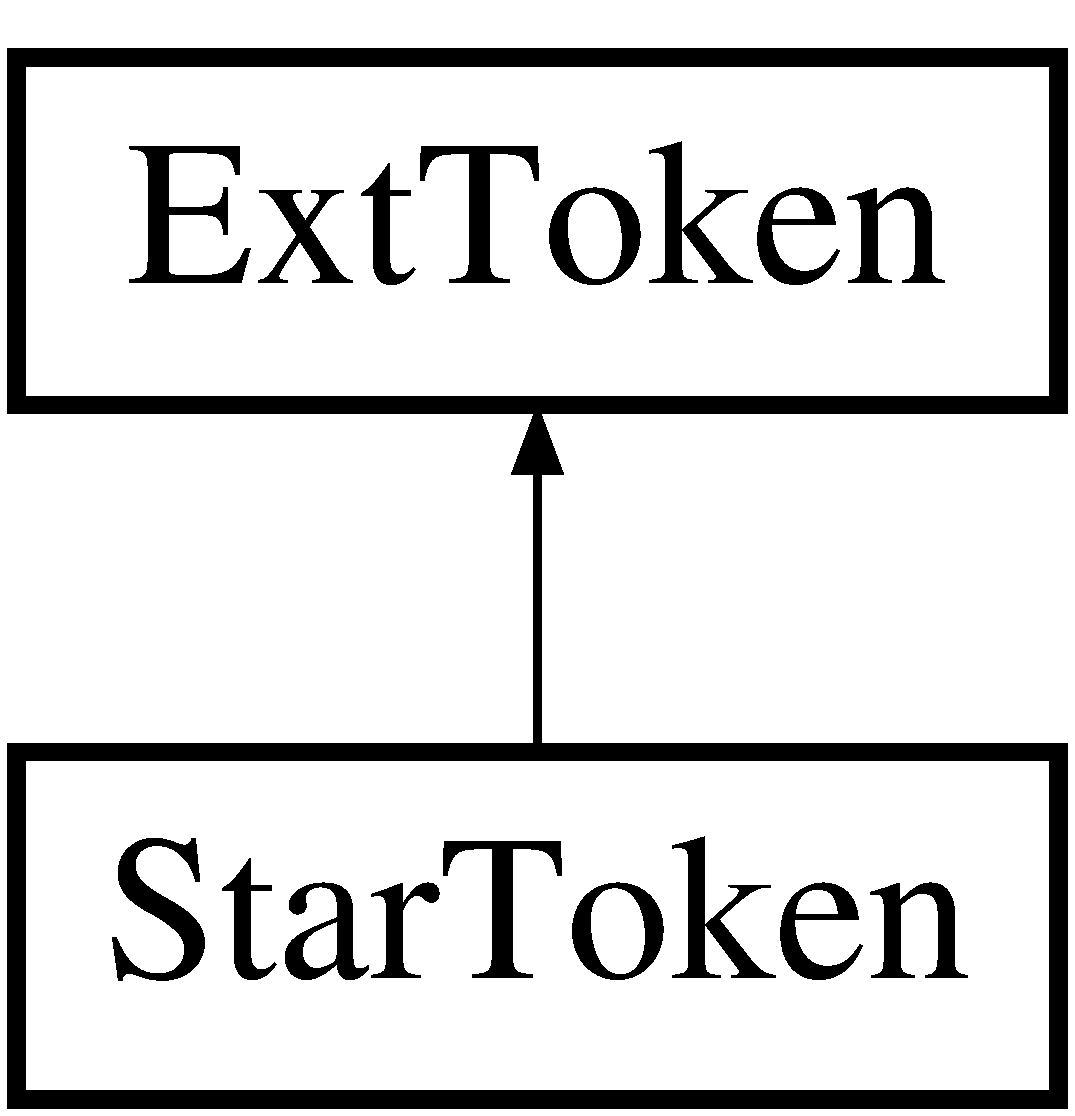
\includegraphics[height=2.000000cm]{classStarToken}
\end{center}
\end{figure}
\subsection*{Public Member Functions}
\begin{DoxyCompactItemize}
\item 
\hypertarget{classStarToken_a9e448a924eb2adbfde602c0590268afd}{{\bfseries Star\-Token} (\hyperlink{classParser}{Parser} $\ast$p, \hyperlink{classToken}{Token} $\ast$t)}\label{classStarToken_a9e448a924eb2adbfde602c0590268afd}

\item 
\hypertarget{classStarToken_aba82bdc81500a58096bfeedad600ad10}{\hyperlink{classParseResult}{Parse\-Result} {\bfseries led} (\hyperlink{classParseResult}{Parse\-Result} left)}\label{classStarToken_aba82bdc81500a58096bfeedad600ad10}

\item 
\hypertarget{classStarToken_a59b81cb08057d75eca4b9a8aad8e2be1}{std\-::string {\bfseries description} ()}\label{classStarToken_a59b81cb08057d75eca4b9a8aad8e2be1}

\item 
\hypertarget{classStarToken_a87682a46d434781795d060e43e7eae23}{int {\bfseries lbp} ()}\label{classStarToken_a87682a46d434781795d060e43e7eae23}

\end{DoxyCompactItemize}
\subsection*{Additional Inherited Members}


The documentation for this class was generated from the following file\-:\begin{DoxyCompactItemize}
\item 
ext\-Token.\-h\end{DoxyCompactItemize}

\hypertarget{classStmt}{\section{Stmt Class Reference}
\label{classStmt}\index{Stmt@{Stmt}}
}
Inheritance diagram for Stmt\-:\begin{figure}[H]
\begin{center}
\leavevmode
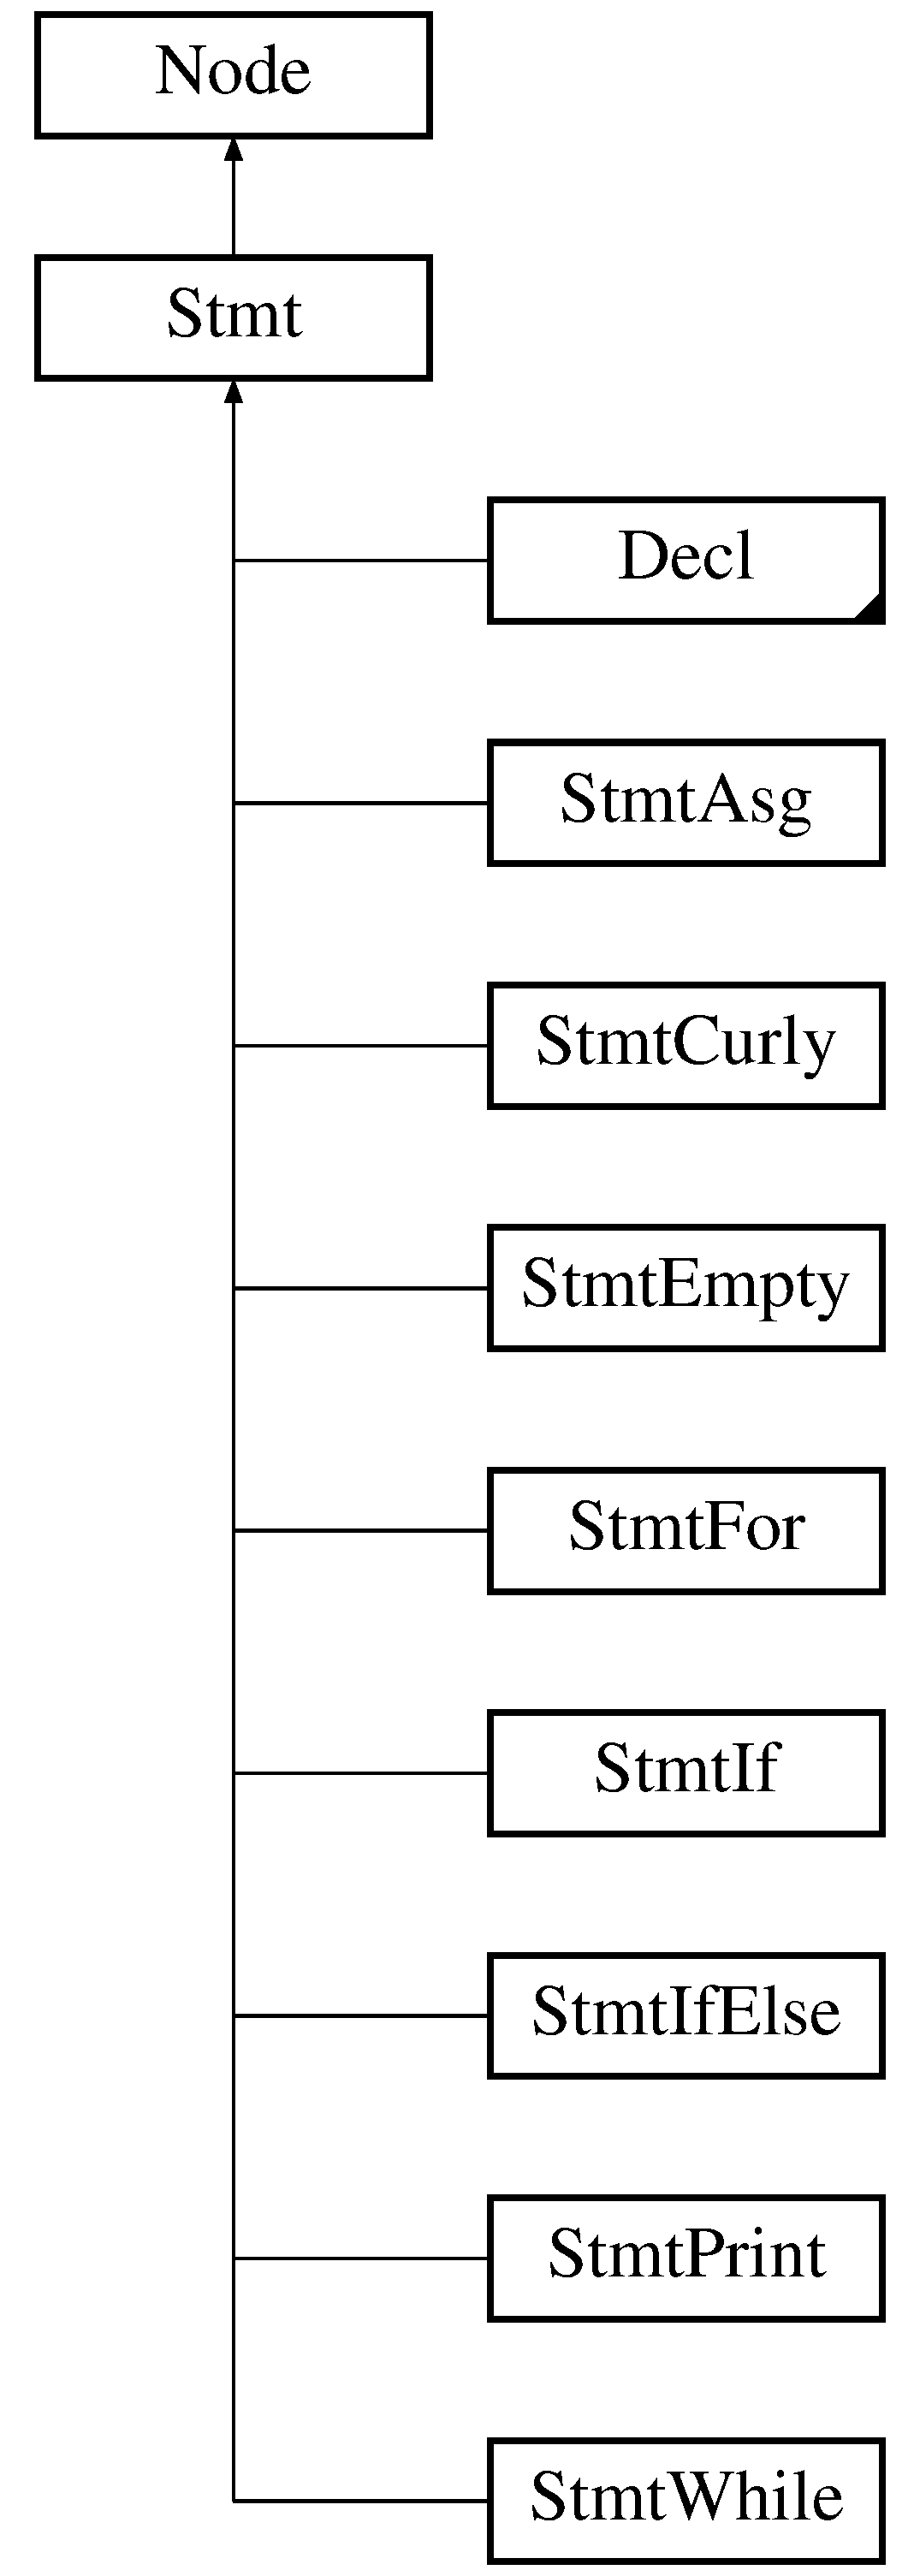
\includegraphics[height=11.000000cm]{classStmt}
\end{center}
\end{figure}
\subsection*{Additional Inherited Members}


The documentation for this class was generated from the following file\-:\begin{DoxyCompactItemize}
\item 
A\-S\-T.\-h\end{DoxyCompactItemize}

\hypertarget{classStmtAsg}{\section{Stmt\-Asg Class Reference}
\label{classStmtAsg}\index{Stmt\-Asg@{Stmt\-Asg}}
}


{\ttfamily \#include $<$A\-S\-T.\-h$>$}

Inheritance diagram for Stmt\-Asg\-:\begin{figure}[H]
\begin{center}
\leavevmode
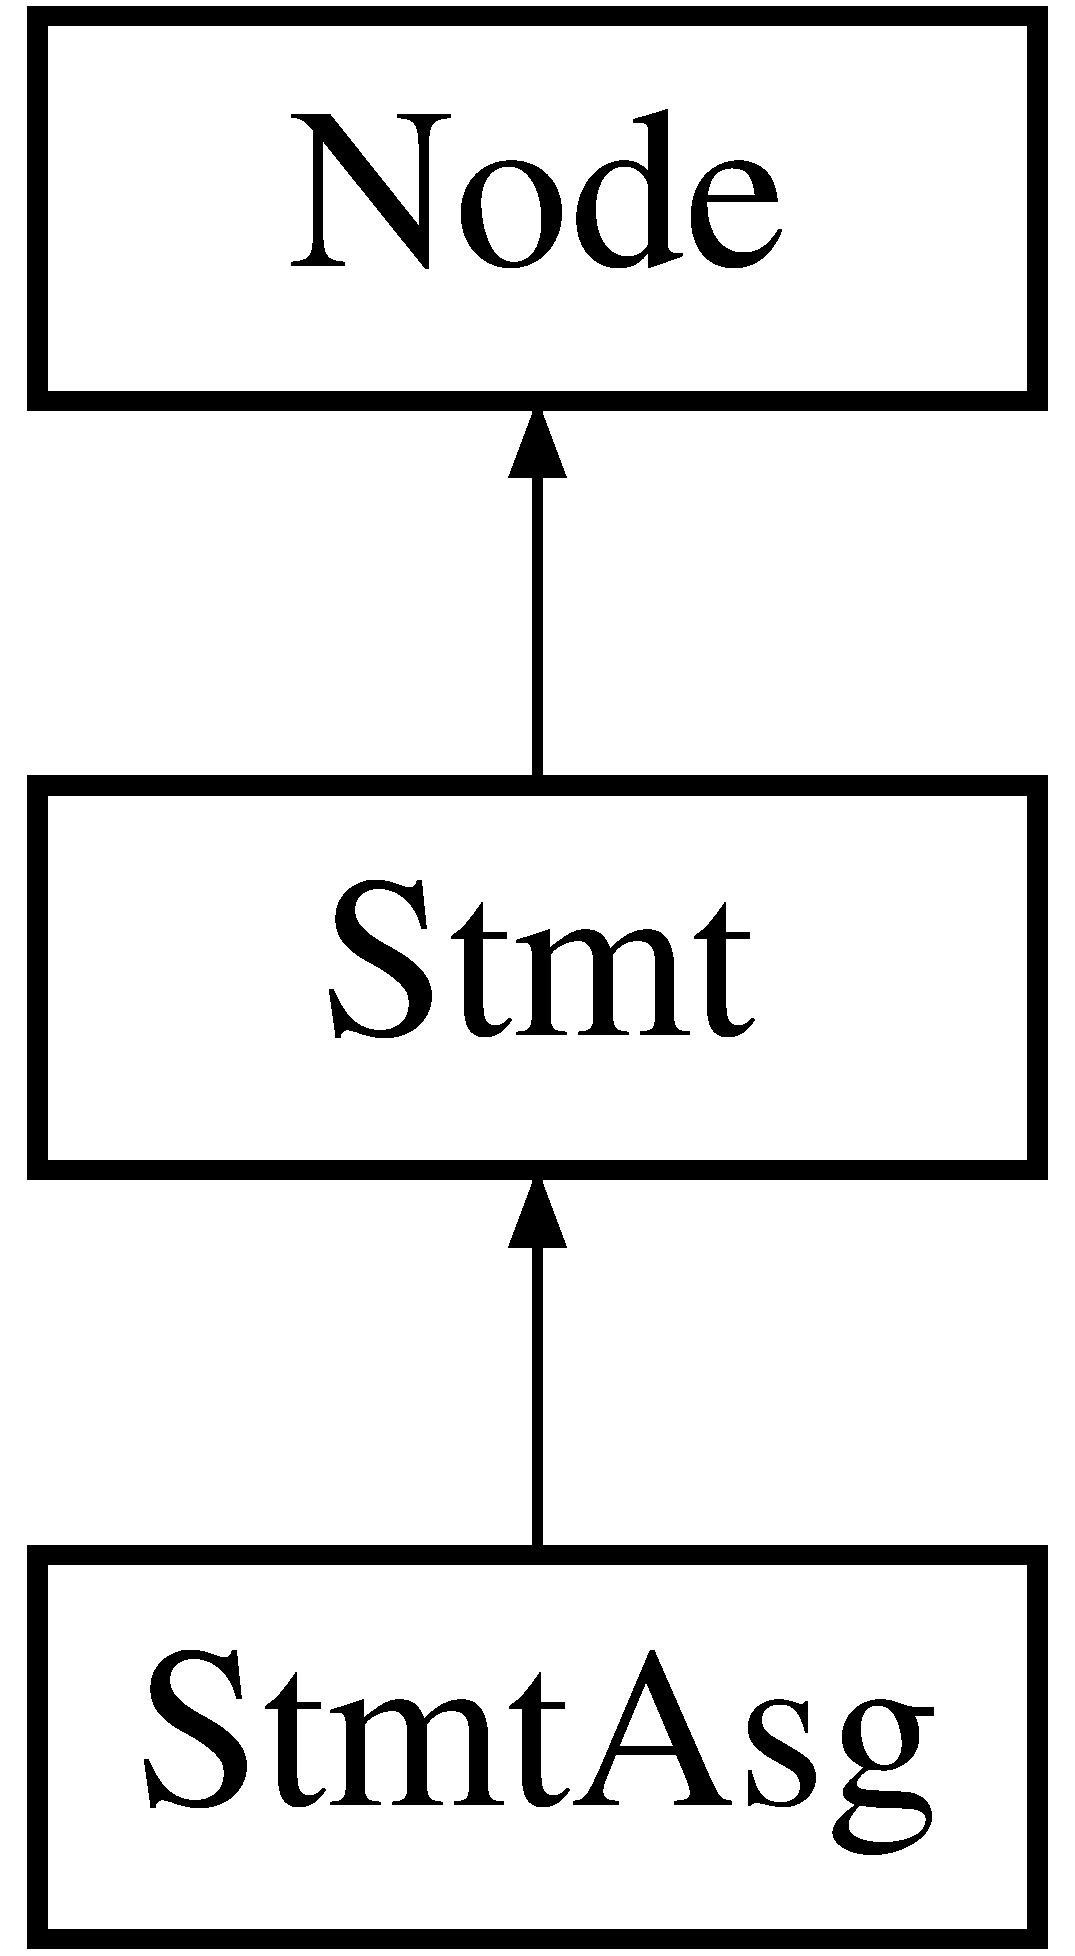
\includegraphics[height=3.000000cm]{classStmtAsg}
\end{center}
\end{figure}
\subsection*{Public Member Functions}
\begin{DoxyCompactItemize}
\item 
\hypertarget{classStmtAsg_a3ba115f325b431815e67cc119445af5d}{{\bfseries Stmt\-Asg} (\hyperlink{classVarname}{Varname} $\ast$\-\_\-varname, \hyperlink{classExpr}{Expr} $\ast$\-\_\-expr)}\label{classStmtAsg_a3ba115f325b431815e67cc119445af5d}

\item 
\hypertarget{classStmtAsg_adec83a1cf5010bdc7863806bd07deb9d}{{\bfseries Stmt\-Asg} (\hyperlink{classVarname}{Varname} $\ast$\-\_\-varname, \hyperlink{classExpr}{Expr} $\ast$\-\_\-expr, \hyperlink{classExpr}{Expr} $\ast$\-\_\-expro, \hyperlink{classExpr}{Expr} $\ast$\-\_\-exprt)}\label{classStmtAsg_adec83a1cf5010bdc7863806bd07deb9d}

\item 
\hypertarget{classStmtAsg_a2a25fa8011c5b33be014e0c1c56bd4d6}{std\-::string {\bfseries unparse} ()}\label{classStmtAsg_a2a25fa8011c5b33be014e0c1c56bd4d6}

\end{DoxyCompactItemize}


\subsection{Detailed Description}
This class below is for an assignment of {\itshape declaration} of variable name and assigning it to an expression 

The documentation for this class was generated from the following file\-:\begin{DoxyCompactItemize}
\item 
A\-S\-T.\-h\end{DoxyCompactItemize}

\hypertarget{classStmtCurly}{\section{Stmt\-Curly Class Reference}
\label{classStmtCurly}\index{Stmt\-Curly@{Stmt\-Curly}}
}


{\ttfamily \#include $<$A\-S\-T.\-h$>$}

Inheritance diagram for Stmt\-Curly\-:\begin{figure}[H]
\begin{center}
\leavevmode
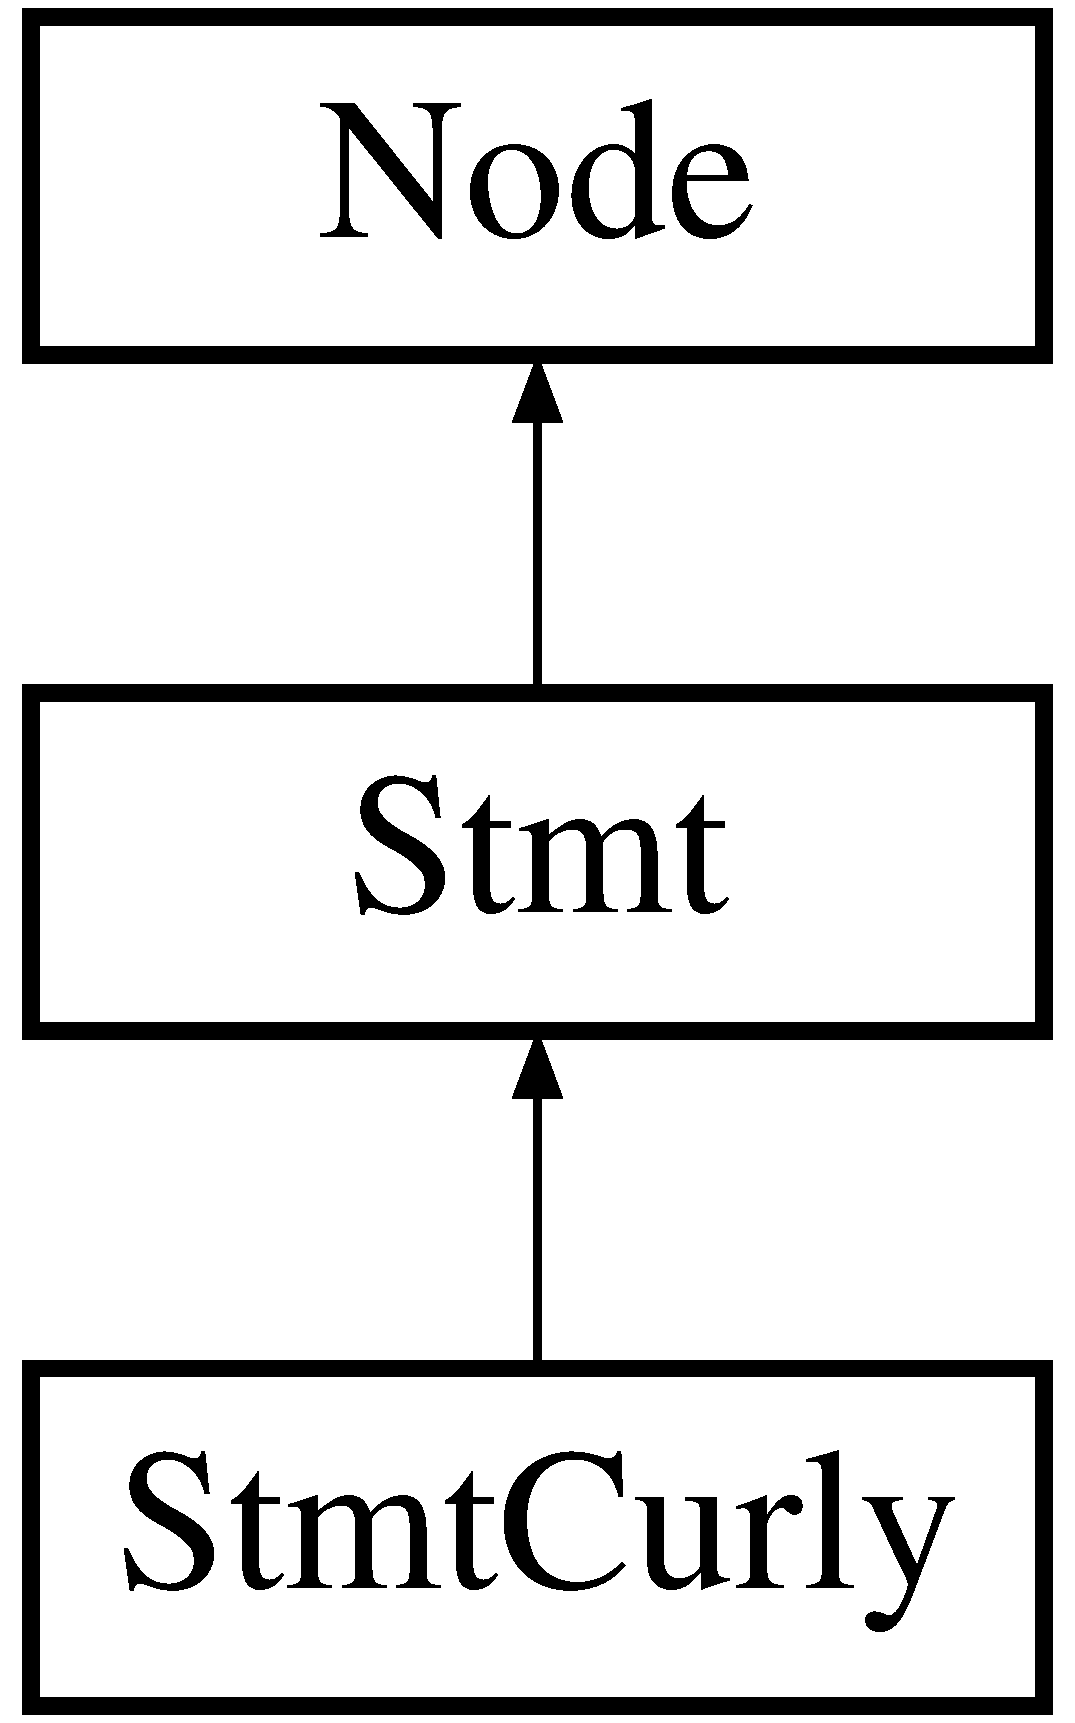
\includegraphics[height=3.000000cm]{classStmtCurly}
\end{center}
\end{figure}
\subsection*{Public Member Functions}
\begin{DoxyCompactItemize}
\item 
\hypertarget{classStmtCurly_a0bd237c8abfe36aca97523792554b758}{{\bfseries Stmt\-Curly} (\hyperlink{classStmts}{Stmts} $\ast$\-\_\-stmts)}\label{classStmtCurly_a0bd237c8abfe36aca97523792554b758}

\item 
\hypertarget{classStmtCurly_a99d6e416a3a1a06034ad9bfa78b8593c}{std\-::string {\bfseries unparse} ()}\label{classStmtCurly_a99d6e416a3a1a06034ad9bfa78b8593c}

\end{DoxyCompactItemize}


\subsection{Detailed Description}
This class is for \hyperlink{classStmts}{Stmts} class that is bound by curly braces 

The documentation for this class was generated from the following file\-:\begin{DoxyCompactItemize}
\item 
A\-S\-T.\-h\end{DoxyCompactItemize}

\hypertarget{classStmtEmpty}{\section{Stmt\-Empty Class Reference}
\label{classStmtEmpty}\index{Stmt\-Empty@{Stmt\-Empty}}
}


{\ttfamily \#include $<$A\-S\-T.\-h$>$}

Inheritance diagram for Stmt\-Empty\-:\begin{figure}[H]
\begin{center}
\leavevmode
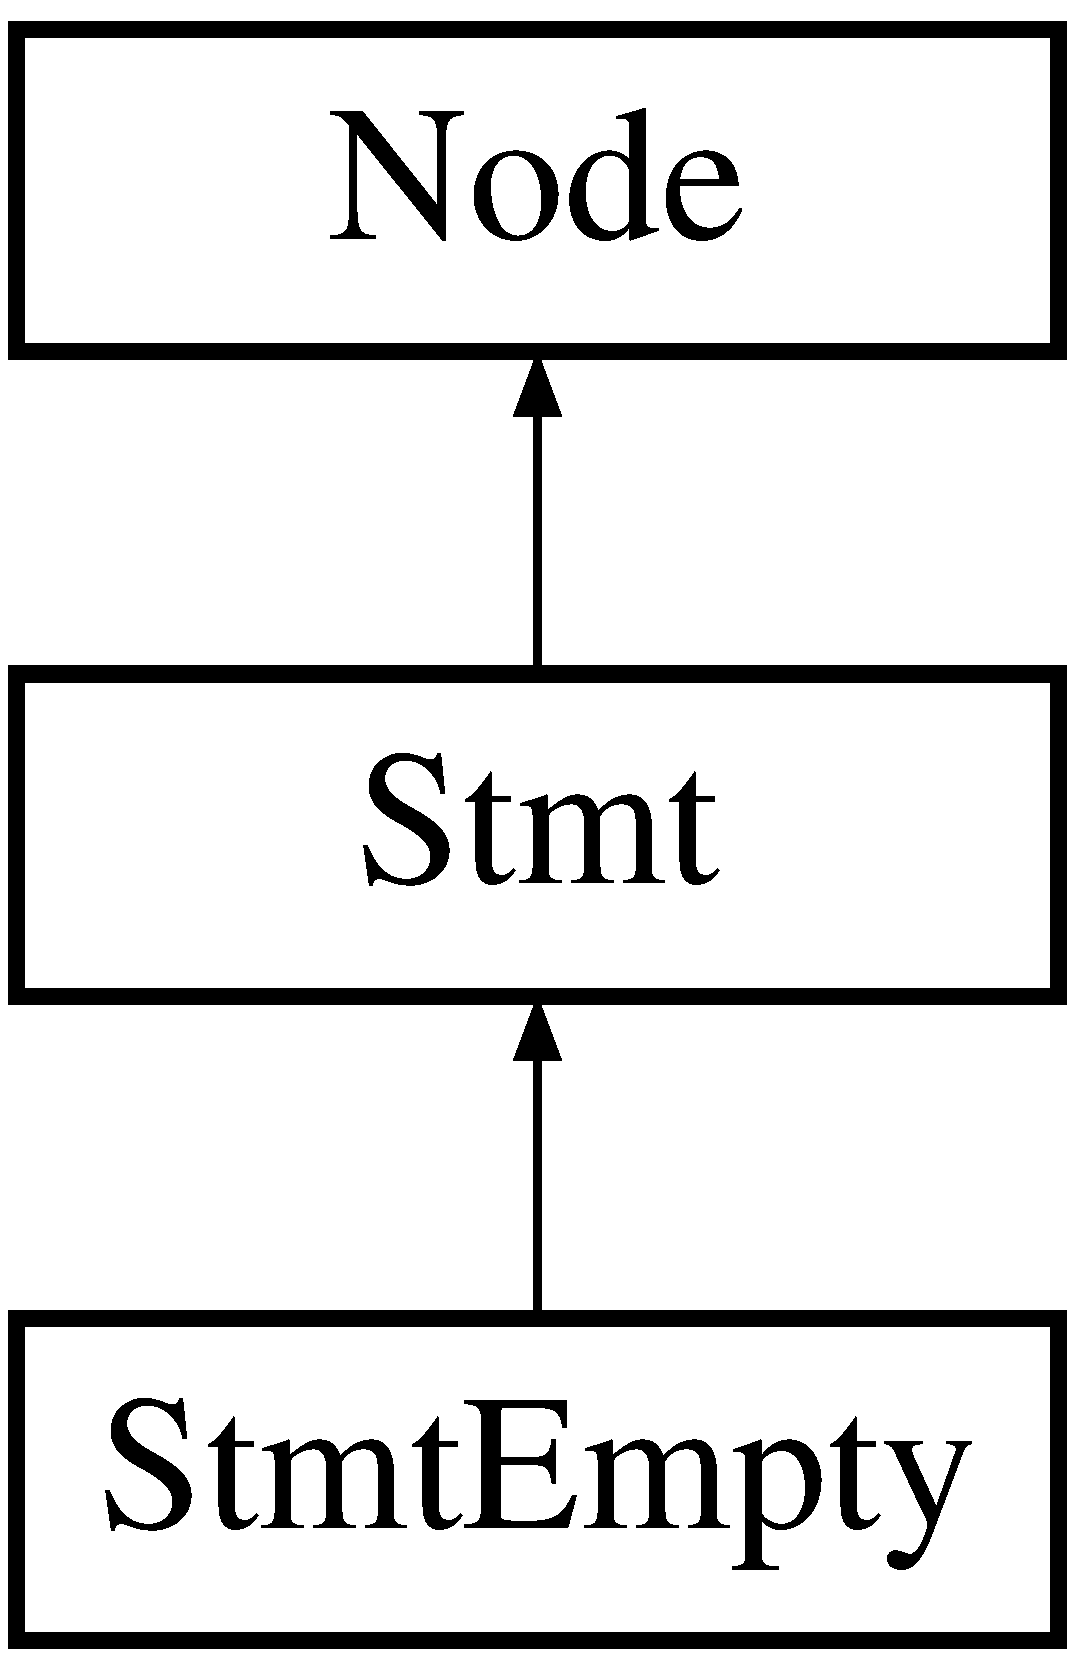
\includegraphics[height=3.000000cm]{classStmtEmpty}
\end{center}
\end{figure}
\subsection*{Public Member Functions}
\begin{DoxyCompactItemize}
\item 
\hypertarget{classStmtEmpty_acb6a58bc9a8734ebc192da9937826273}{std\-::string {\bfseries unparse} ()}\label{classStmtEmpty_acb6a58bc9a8734ebc192da9937826273}

\end{DoxyCompactItemize}


\subsection{Detailed Description}
We call this the empty statement because when we unparse is, it just has a semi-\/colon,  it doesn't have any statements (end) 

The documentation for this class was generated from the following file\-:\begin{DoxyCompactItemize}
\item 
A\-S\-T.\-h\end{DoxyCompactItemize}

\hypertarget{classStmtFor}{\section{Stmt\-For Class Reference}
\label{classStmtFor}\index{Stmt\-For@{Stmt\-For}}
}


{\ttfamily \#include $<$A\-S\-T.\-h$>$}

Inheritance diagram for Stmt\-For\-:\begin{figure}[H]
\begin{center}
\leavevmode
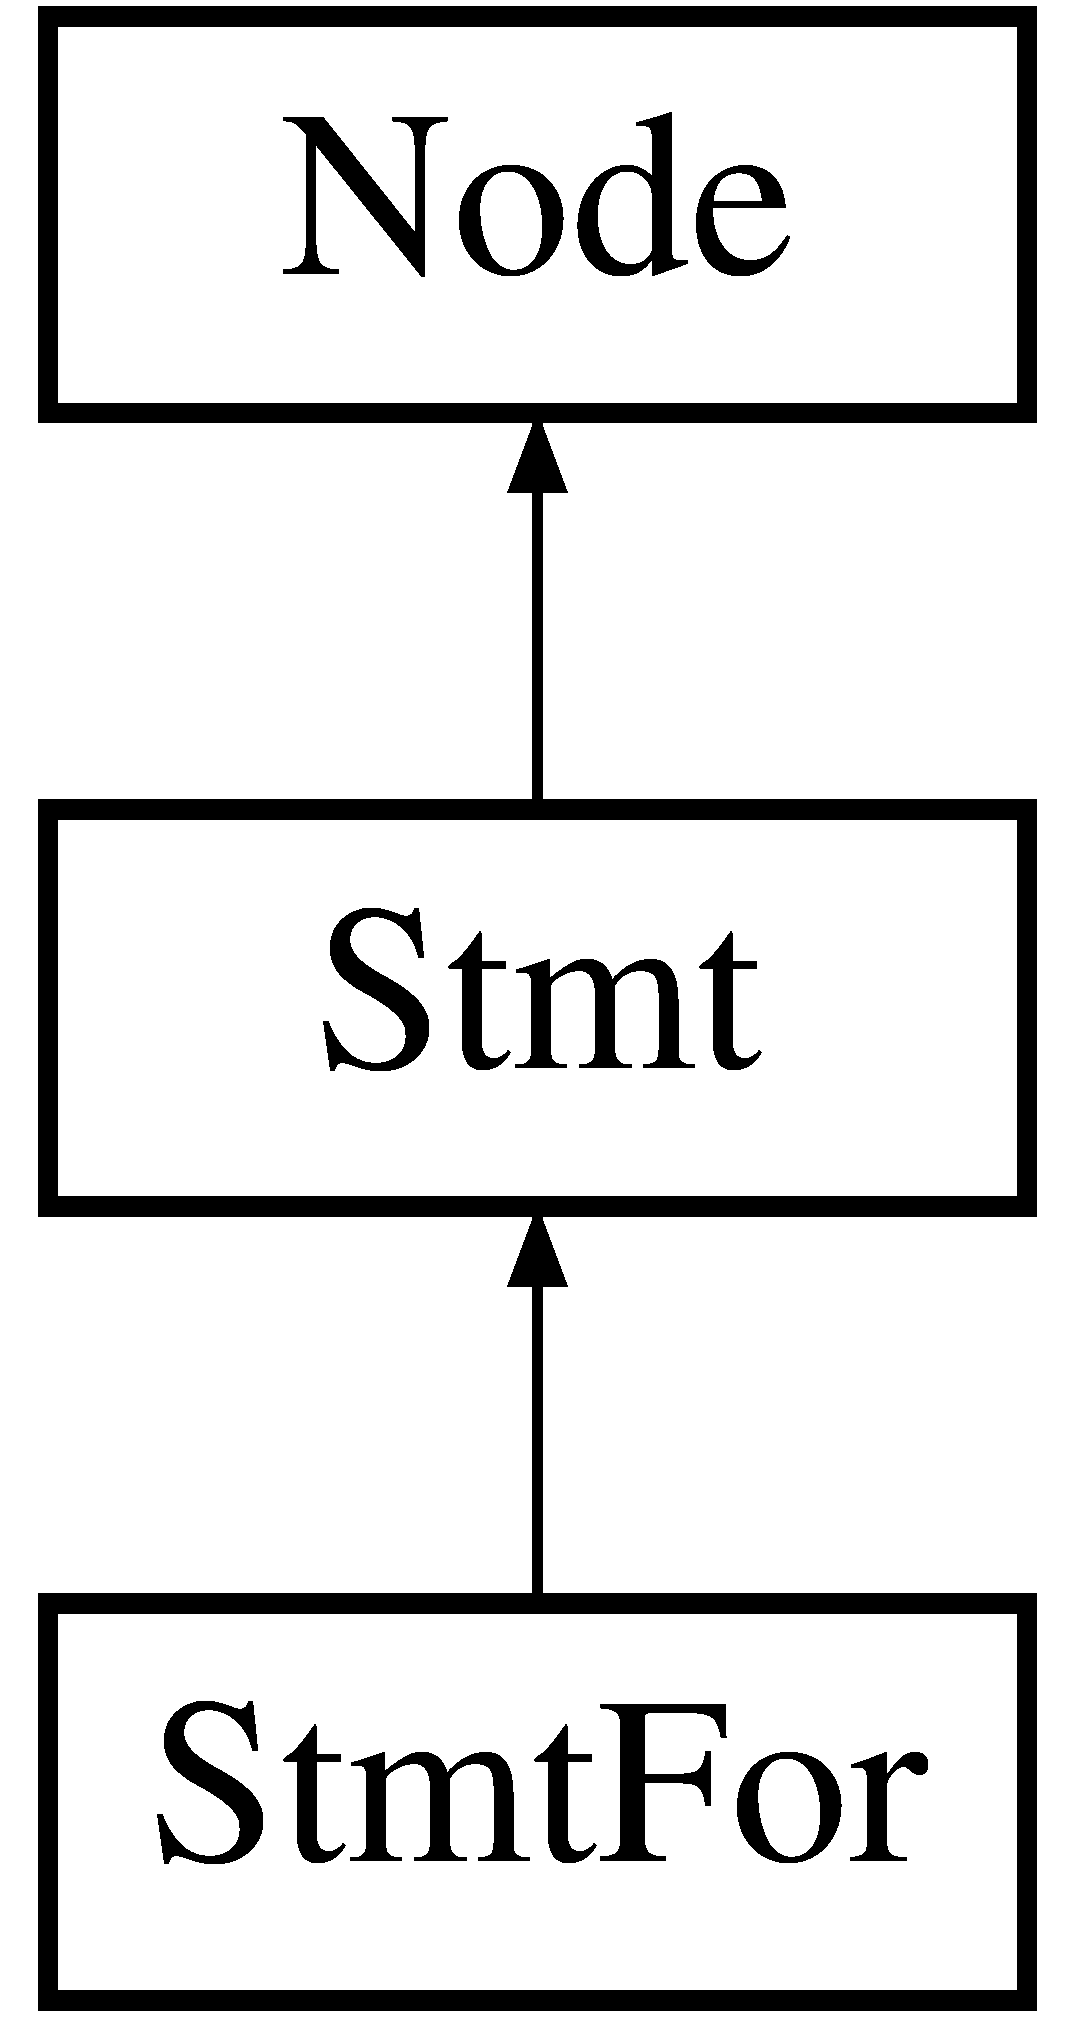
\includegraphics[height=3.000000cm]{classStmtFor}
\end{center}
\end{figure}
\subsection*{Public Member Functions}
\begin{DoxyCompactItemize}
\item 
\hypertarget{classStmtFor_adf16f36352035a80f470b9b655fc2c91}{{\bfseries Stmt\-For} (\hyperlink{classVarname}{Varname} $\ast$\-\_\-v, \hyperlink{classExpr}{Expr} $\ast$\-\_\-e, \hyperlink{classExpr}{Expr} $\ast$\-\_\-s, \hyperlink{classStmt}{Stmt} $\ast$\-\_\-ss)}\label{classStmtFor_adf16f36352035a80f470b9b655fc2c91}

\item 
\hypertarget{classStmtFor_a91c8475d4d4628fed8926ffc22425b95}{std\-::string {\bfseries unparse} ()}\label{classStmtFor_a91c8475d4d4628fed8926ffc22425b95}

\end{DoxyCompactItemize}


\subsection{Detailed Description}
This class is for a for-\/loop statement 

The documentation for this class was generated from the following file\-:\begin{DoxyCompactItemize}
\item 
A\-S\-T.\-h\end{DoxyCompactItemize}

\hypertarget{classStmtIf}{\section{Stmt\-If Class Reference}
\label{classStmtIf}\index{Stmt\-If@{Stmt\-If}}
}


{\ttfamily \#include $<$A\-S\-T.\-h$>$}

Inheritance diagram for Stmt\-If\-:\begin{figure}[H]
\begin{center}
\leavevmode
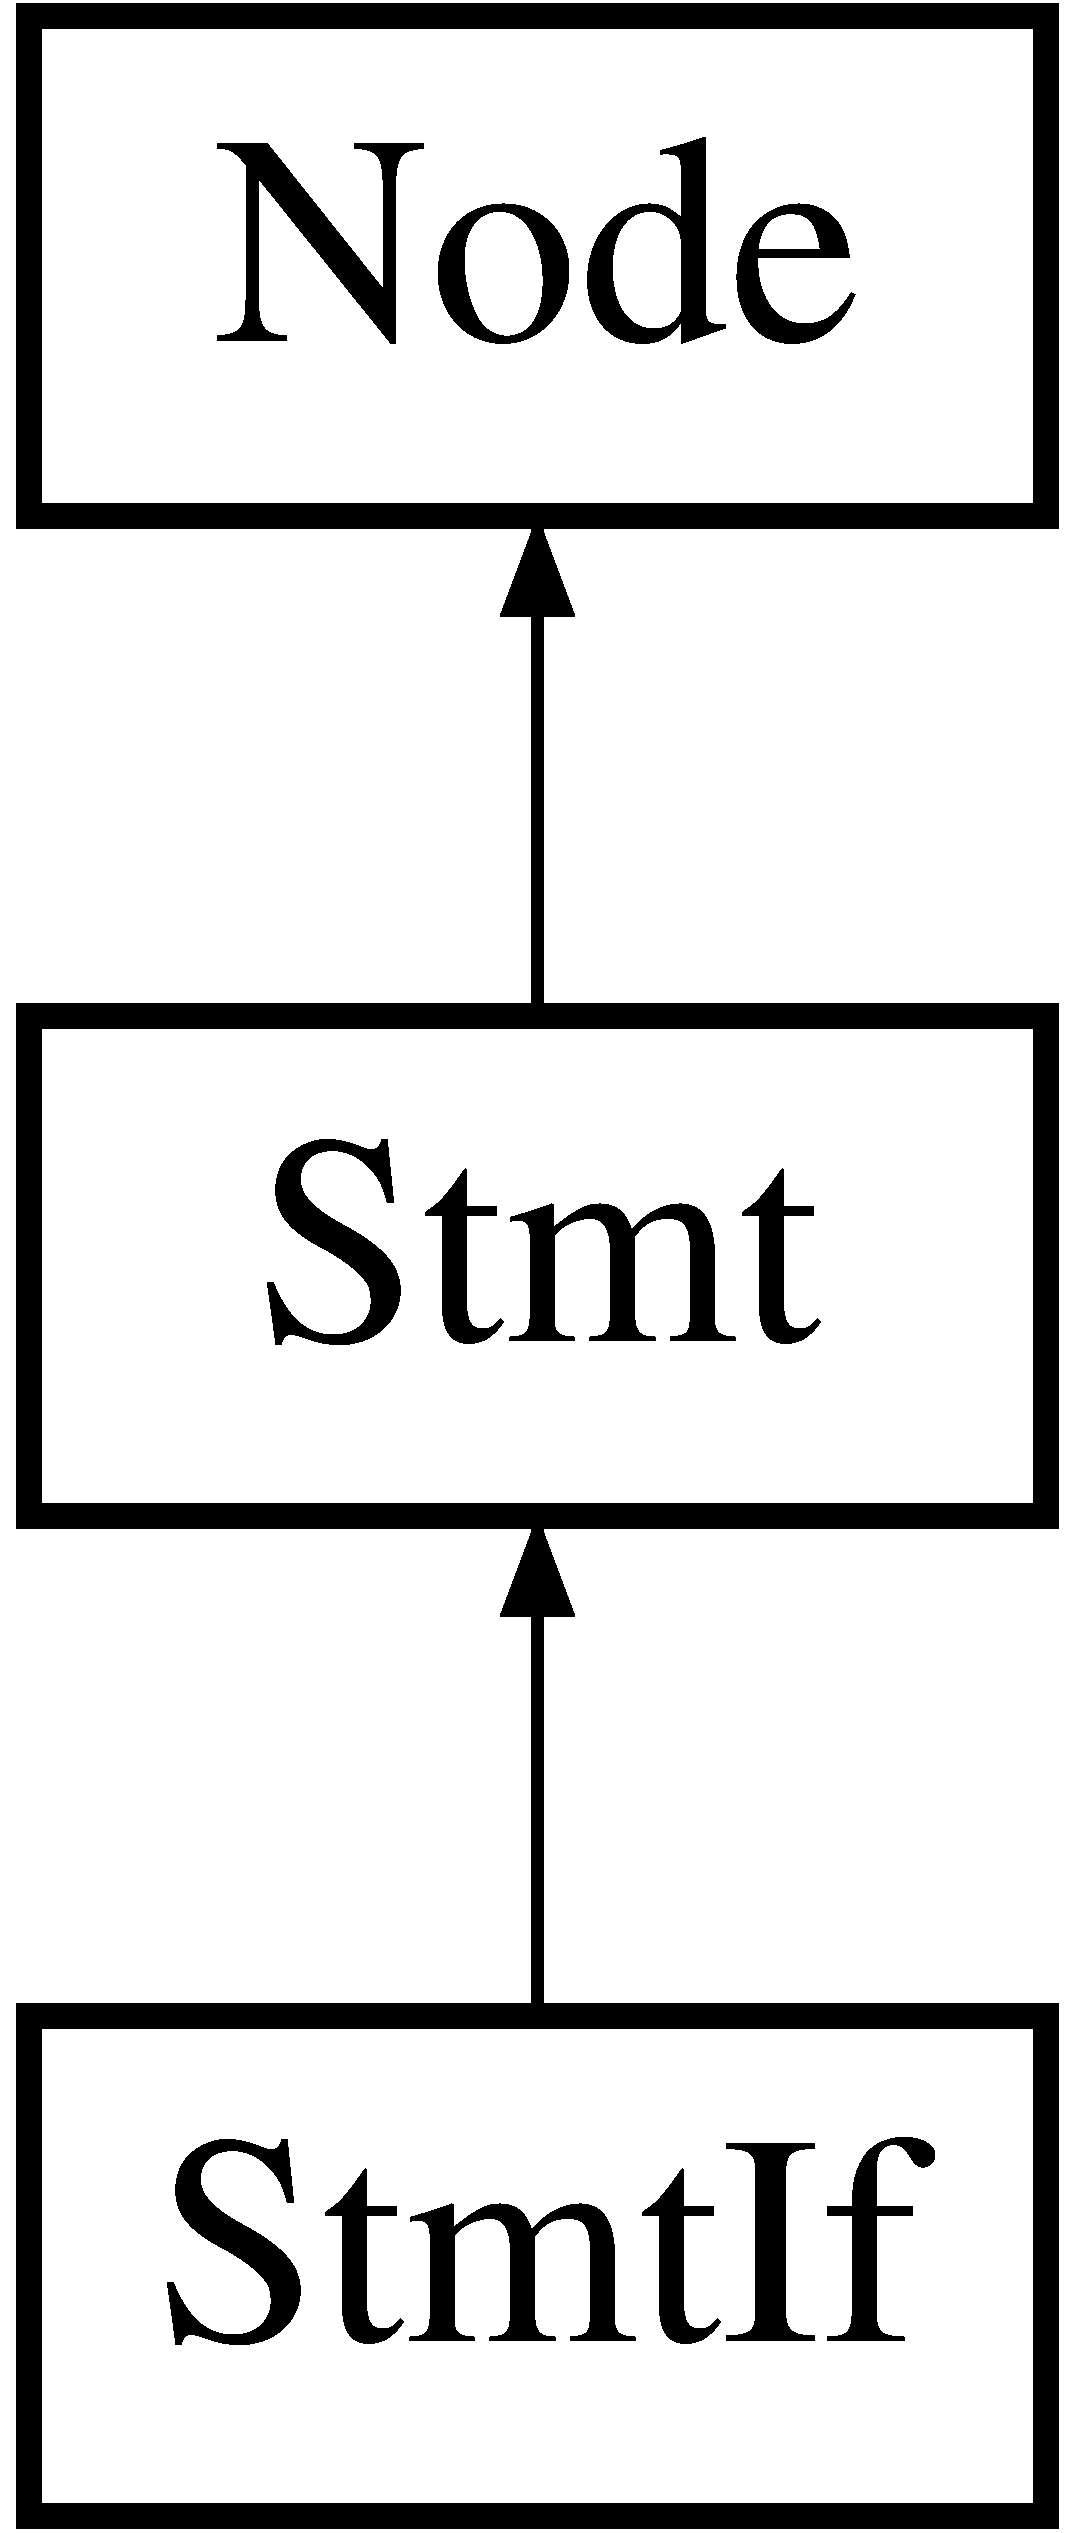
\includegraphics[height=3.000000cm]{classStmtIf}
\end{center}
\end{figure}
\subsection*{Public Member Functions}
\begin{DoxyCompactItemize}
\item 
\hypertarget{classStmtIf_a854063cee761f01d67a0f1cec9d8f2d8}{{\bfseries Stmt\-If} (\hyperlink{classExpr}{Expr} $\ast$\-\_\-expr, \hyperlink{classStmt}{Stmt} $\ast$\-\_\-stmt)}\label{classStmtIf_a854063cee761f01d67a0f1cec9d8f2d8}

\item 
\hypertarget{classStmtIf_a6d74da2991d585ee7ccf23e81d4de602}{std\-::string {\bfseries unparse} ()}\label{classStmtIf_a6d74da2991d585ee7ccf23e81d4de602}

\end{DoxyCompactItemize}


\subsection{Detailed Description}
This class below is for an if-\/statement 

The documentation for this class was generated from the following file\-:\begin{DoxyCompactItemize}
\item 
A\-S\-T.\-h\end{DoxyCompactItemize}

\hypertarget{classStmtIfElse}{\section{Stmt\-If\-Else Class Reference}
\label{classStmtIfElse}\index{Stmt\-If\-Else@{Stmt\-If\-Else}}
}


{\ttfamily \#include $<$A\-S\-T.\-h$>$}

Inheritance diagram for Stmt\-If\-Else\-:\begin{figure}[H]
\begin{center}
\leavevmode
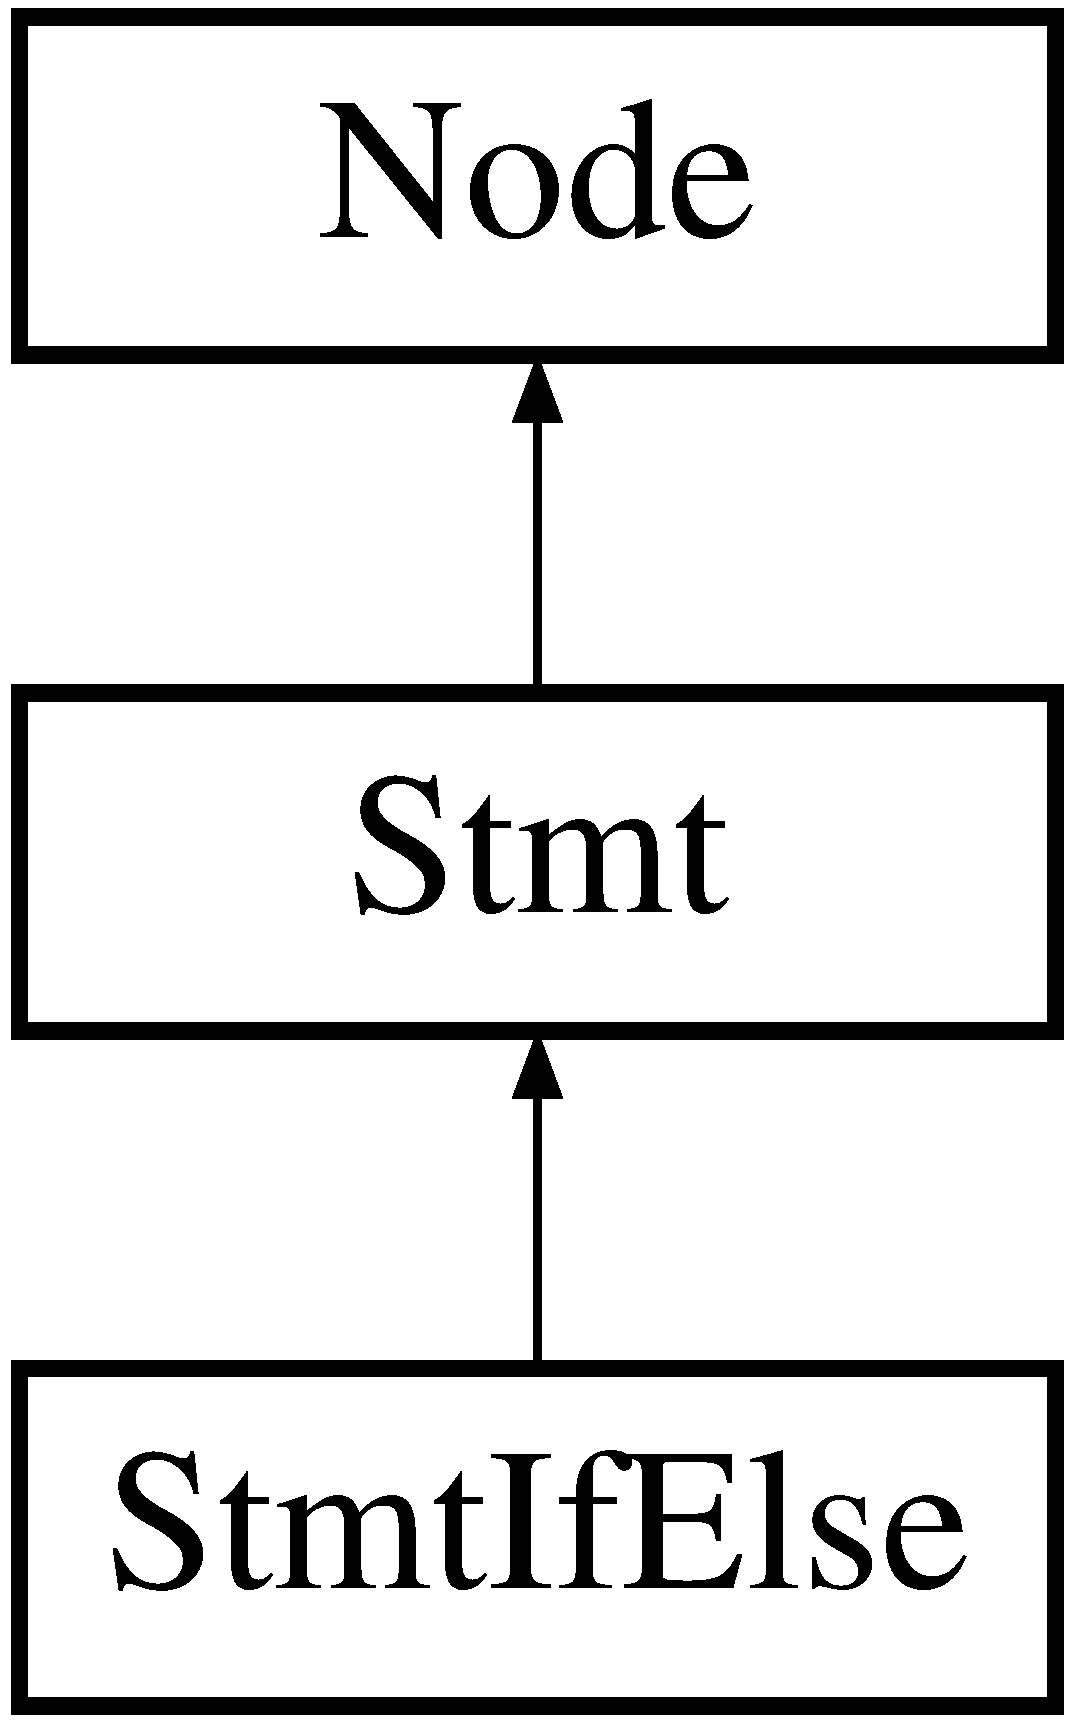
\includegraphics[height=3.000000cm]{classStmtIfElse}
\end{center}
\end{figure}
\subsection*{Public Member Functions}
\begin{DoxyCompactItemize}
\item 
\hypertarget{classStmtIfElse_ae2f0b979cf81a33f9e14fe66d160d566}{{\bfseries Stmt\-If\-Else} (\hyperlink{classExpr}{Expr} $\ast$\-\_\-expr, \hyperlink{classStmt}{Stmt} $\ast$\-\_\-left, \hyperlink{classStmt}{Stmt} $\ast$\-\_\-right)}\label{classStmtIfElse_ae2f0b979cf81a33f9e14fe66d160d566}

\item 
\hypertarget{classStmtIfElse_a276e62a0a9f70ba8e50b0e1d080265a8}{std\-::string {\bfseries unparse} ()}\label{classStmtIfElse_a276e62a0a9f70ba8e50b0e1d080265a8}

\end{DoxyCompactItemize}


\subsection{Detailed Description}
This class below is for an if-\/else statement 

The documentation for this class was generated from the following file\-:\begin{DoxyCompactItemize}
\item 
A\-S\-T.\-h\end{DoxyCompactItemize}

\hypertarget{classStmtPrint}{\section{Stmt\-Print Class Reference}
\label{classStmtPrint}\index{Stmt\-Print@{Stmt\-Print}}
}


{\ttfamily \#include $<$A\-S\-T.\-h$>$}

Inheritance diagram for Stmt\-Print\-:\begin{figure}[H]
\begin{center}
\leavevmode
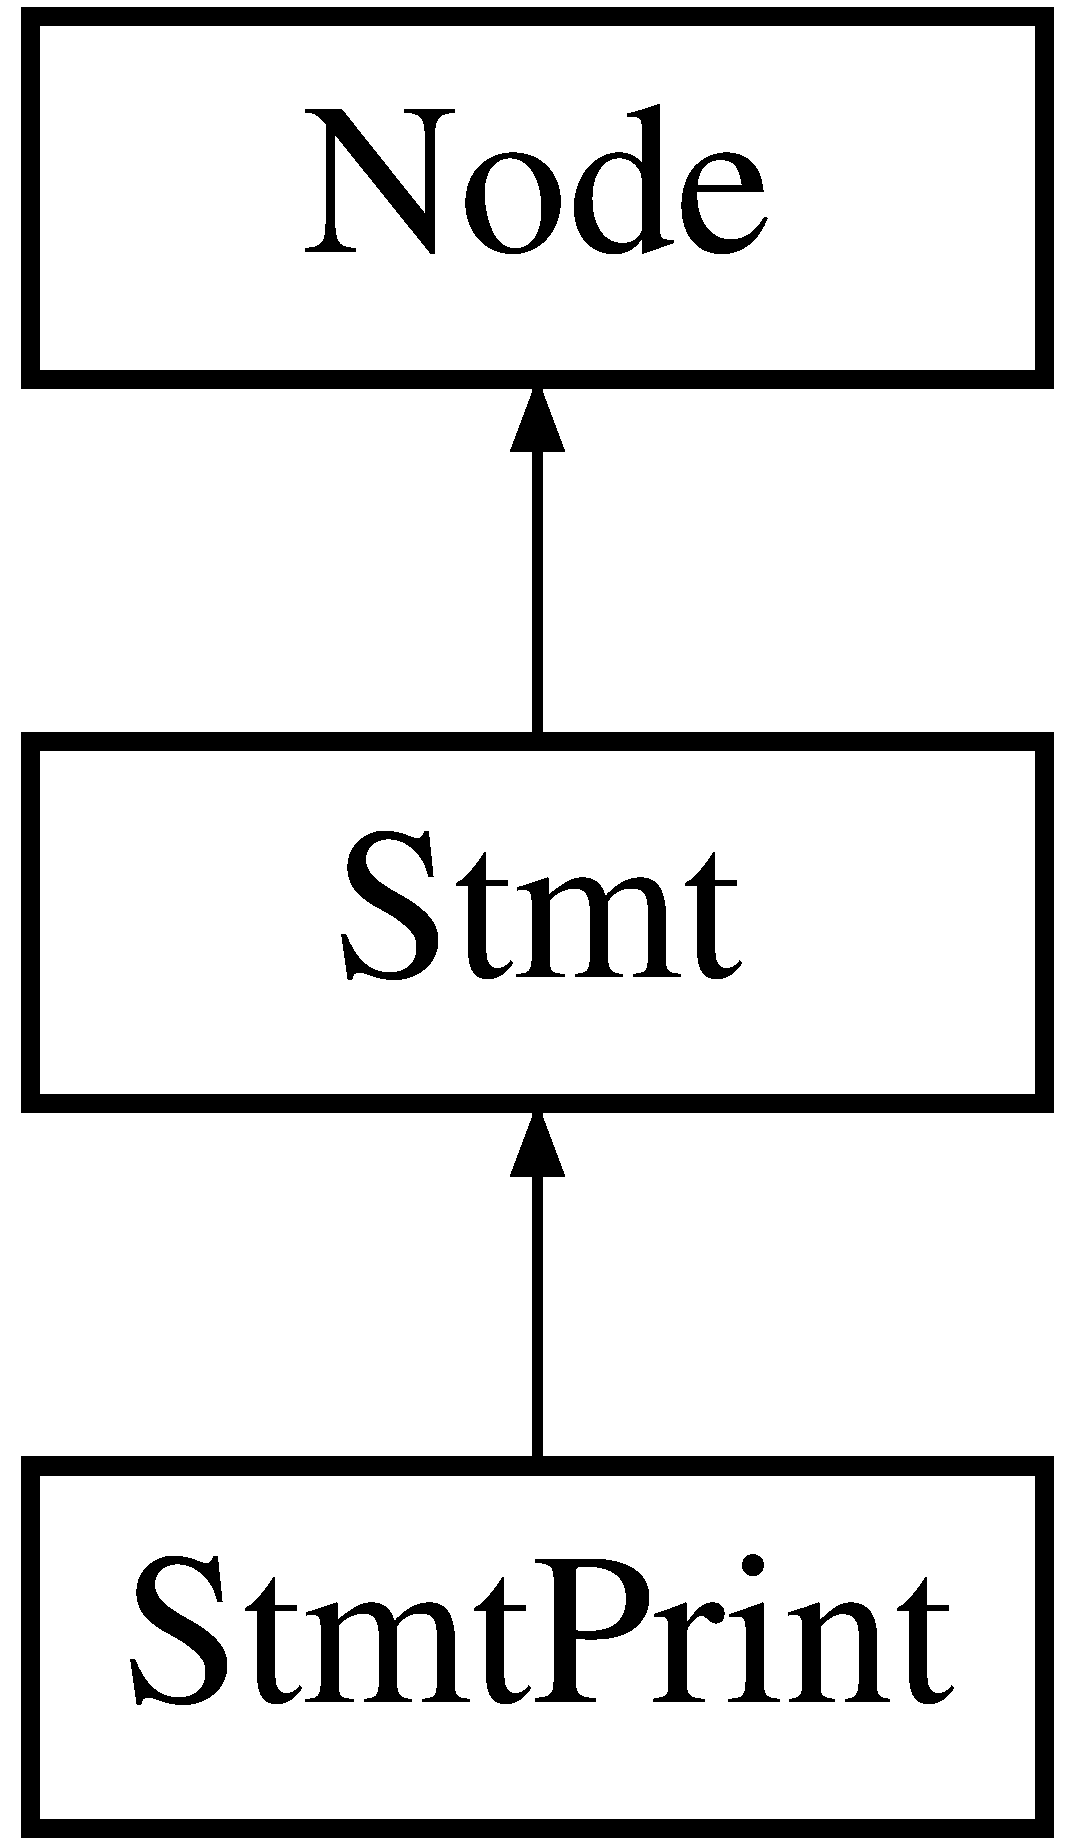
\includegraphics[height=3.000000cm]{classStmtPrint}
\end{center}
\end{figure}
\subsection*{Public Member Functions}
\begin{DoxyCompactItemize}
\item 
\hypertarget{classStmtPrint_a9ca7ffa218050c250cdce704bcaf1c89}{{\bfseries Stmt\-Print} (\hyperlink{classExpr}{Expr} $\ast$\-\_\-expr)}\label{classStmtPrint_a9ca7ffa218050c250cdce704bcaf1c89}

\item 
\hypertarget{classStmtPrint_adf9cf968194ef383115d2043f5bba6a3}{std\-::string {\bfseries unparse} ()}\label{classStmtPrint_adf9cf968194ef383115d2043f5bba6a3}

\end{DoxyCompactItemize}


\subsection{Detailed Description}
This class is for the print terminal. Note, it does not actually print anything, 

The documentation for this class was generated from the following files\-:\begin{DoxyCompactItemize}
\item 
A\-S\-T.\-h\item 
A\-S\-T.\-cpp\end{DoxyCompactItemize}

\hypertarget{classStmts}{\section{Stmts Class Reference}
\label{classStmts}\index{Stmts@{Stmts}}
}
Inheritance diagram for Stmts\-:\begin{figure}[H]
\begin{center}
\leavevmode
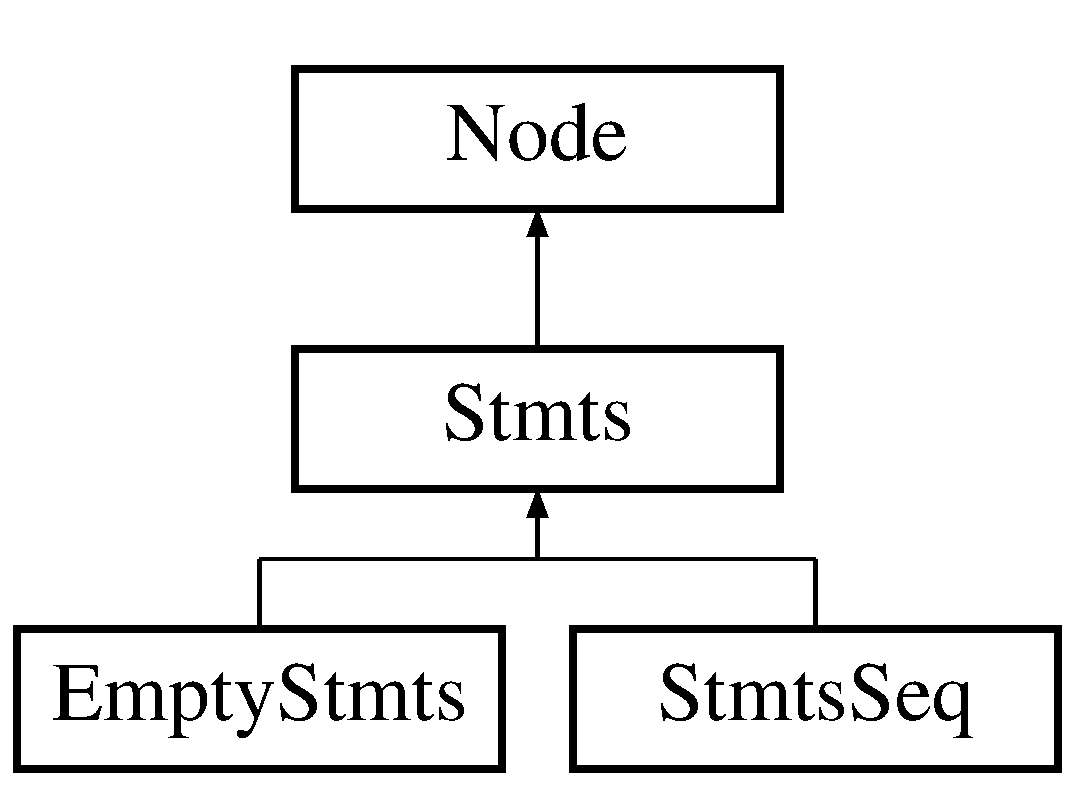
\includegraphics[height=3.000000cm]{classStmts}
\end{center}
\end{figure}
\subsection*{Public Member Functions}
\begin{DoxyCompactItemize}
\item 
\hypertarget{classStmts_a9967fb1509f331485ba359cd8745fc82}{virtual std\-::string {\bfseries unparse} ()=0}\label{classStmts_a9967fb1509f331485ba359cd8745fc82}

\end{DoxyCompactItemize}


The documentation for this class was generated from the following file\-:\begin{DoxyCompactItemize}
\item 
A\-S\-T.\-h\end{DoxyCompactItemize}

\hypertarget{classStmtsSeq}{\section{Stmts\-Seq Class Reference}
\label{classStmtsSeq}\index{Stmts\-Seq@{Stmts\-Seq}}
}


{\ttfamily \#include $<$A\-S\-T.\-h$>$}

Inheritance diagram for Stmts\-Seq\-:\begin{figure}[H]
\begin{center}
\leavevmode
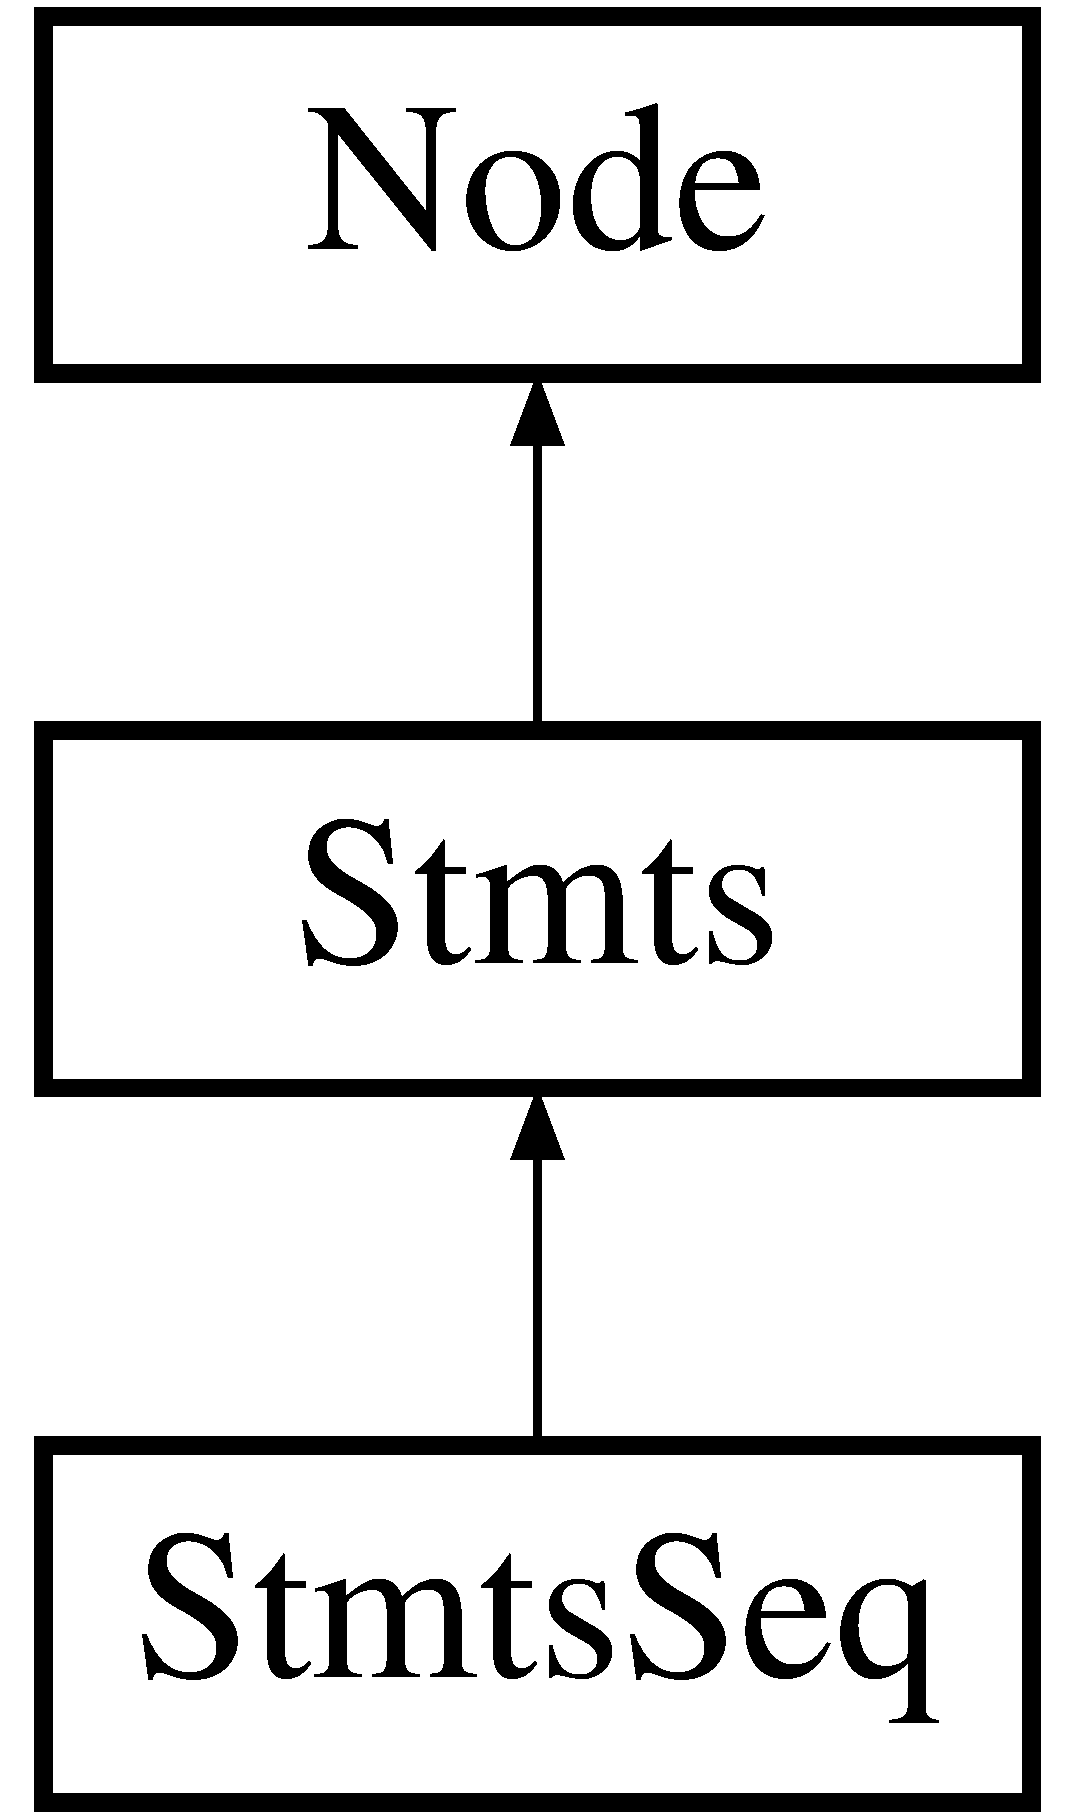
\includegraphics[height=3.000000cm]{classStmtsSeq}
\end{center}
\end{figure}
\subsection*{Public Member Functions}
\begin{DoxyCompactItemize}
\item 
\hypertarget{classStmtsSeq_a4712f47aa19254d0c5fdece5c83a8b3a}{{\bfseries Stmts\-Seq} (\hyperlink{classStmt}{Stmt} $\ast$\-\_\-stmt, \hyperlink{classStmts}{Stmts} $\ast$\-\_\-stmts)}\label{classStmtsSeq_a4712f47aa19254d0c5fdece5c83a8b3a}

\item 
\hypertarget{classStmtsSeq_ad717a80bb854d28a9621e9921d01ba7f}{std\-::string {\bfseries unparse} ()}\label{classStmtsSeq_ad717a80bb854d28a9621e9921d01ba7f}

\end{DoxyCompactItemize}


\subsection{Detailed Description}
This class allows a sequence of many \hyperlink{classStmt}{Stmt} bundled into a \hyperlink{classStmts}{Stmts} tree(or branch) 

The documentation for this class was generated from the following files\-:\begin{DoxyCompactItemize}
\item 
A\-S\-T.\-h\item 
A\-S\-T.\-cpp\end{DoxyCompactItemize}

\hypertarget{classStmtWhile}{\section{Stmt\-While Class Reference}
\label{classStmtWhile}\index{Stmt\-While@{Stmt\-While}}
}


{\ttfamily \#include $<$A\-S\-T.\-h$>$}

Inheritance diagram for Stmt\-While\-:\begin{figure}[H]
\begin{center}
\leavevmode
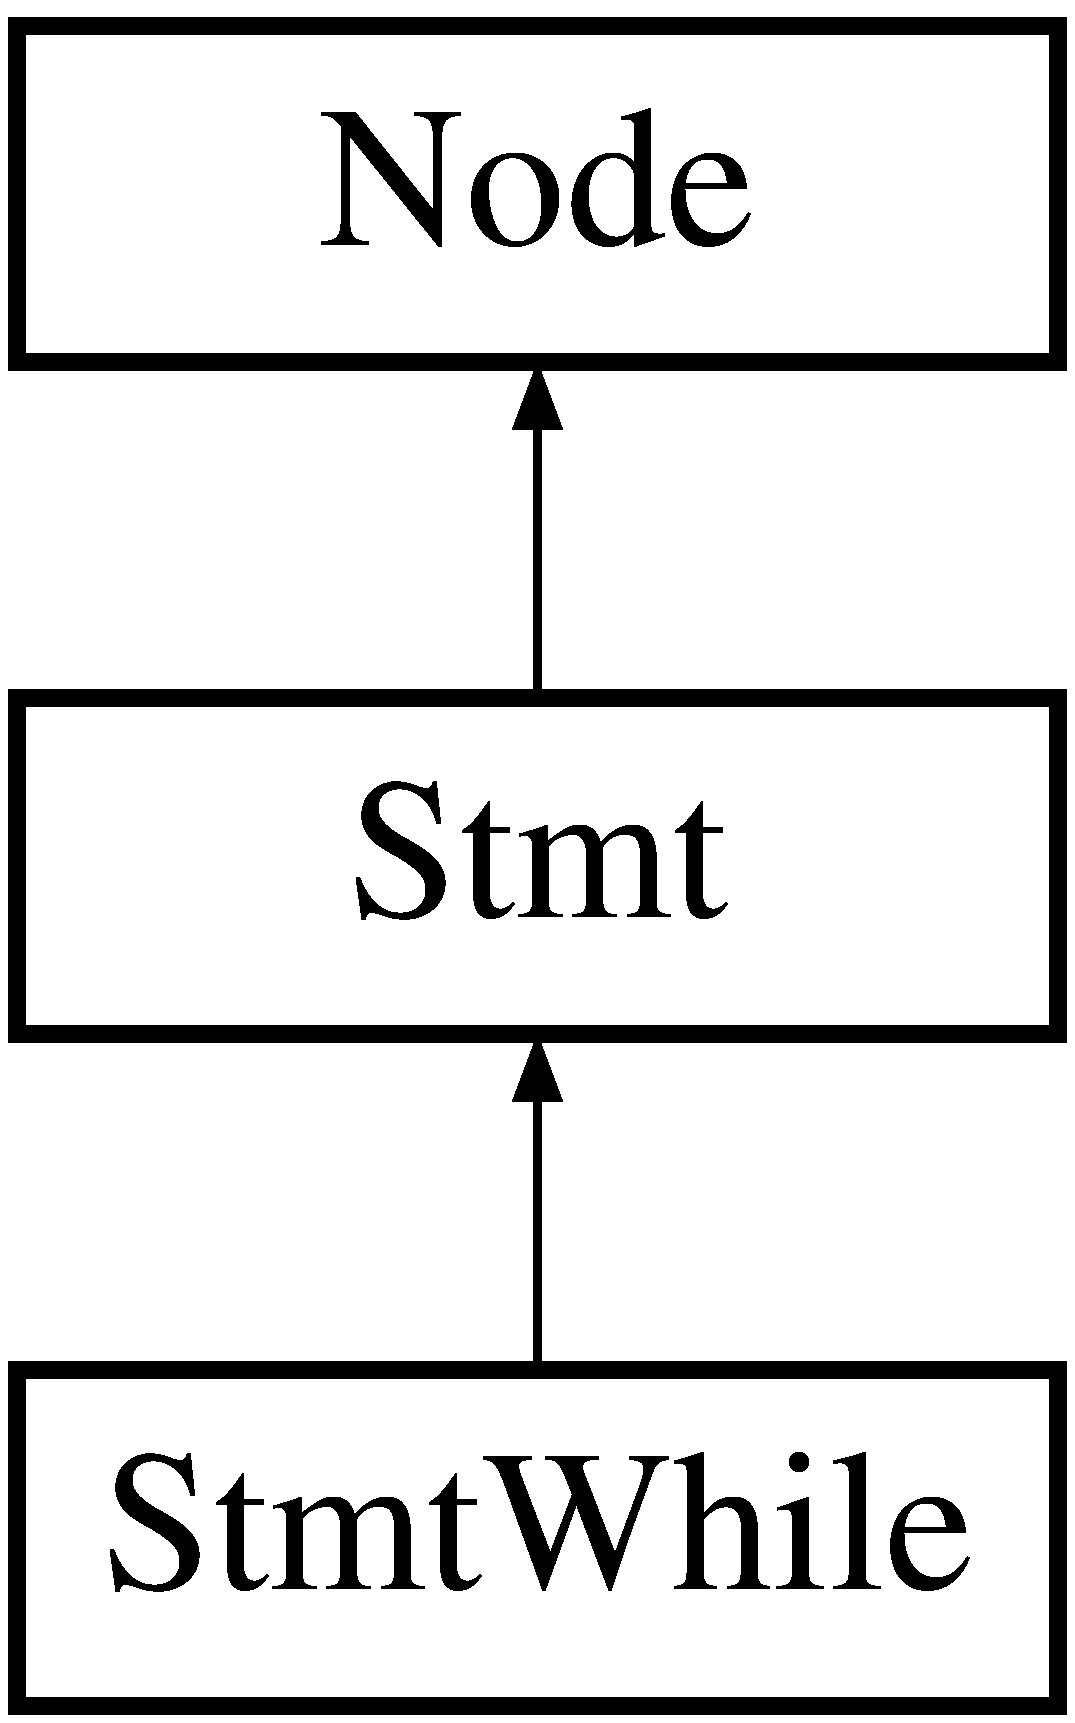
\includegraphics[height=3.000000cm]{classStmtWhile}
\end{center}
\end{figure}
\subsection*{Public Member Functions}
\begin{DoxyCompactItemize}
\item 
\hypertarget{classStmtWhile_a022ea802e57d9de4d664cfd0a97ffcb4}{{\bfseries Stmt\-While} (\hyperlink{classExpr}{Expr} $\ast$\-\_\-e, \hyperlink{classStmt}{Stmt} $\ast$\-\_\-s)}\label{classStmtWhile_a022ea802e57d9de4d664cfd0a97ffcb4}

\item 
\hypertarget{classStmtWhile_a832f826fc3a07af5fb82407bf60ba5ce}{std\-::string {\bfseries unparse} ()}\label{classStmtWhile_a832f826fc3a07af5fb82407bf60ba5ce}

\end{DoxyCompactItemize}


\subsection{Detailed Description}
This class is for a while loop statement 

The documentation for this class was generated from the following file\-:\begin{DoxyCompactItemize}
\item 
A\-S\-T.\-h\end{DoxyCompactItemize}

\hypertarget{classStringConstToken}{\section{String\-Const\-Token Class Reference}
\label{classStringConstToken}\index{String\-Const\-Token@{String\-Const\-Token}}
}
Inheritance diagram for String\-Const\-Token\-:\begin{figure}[H]
\begin{center}
\leavevmode
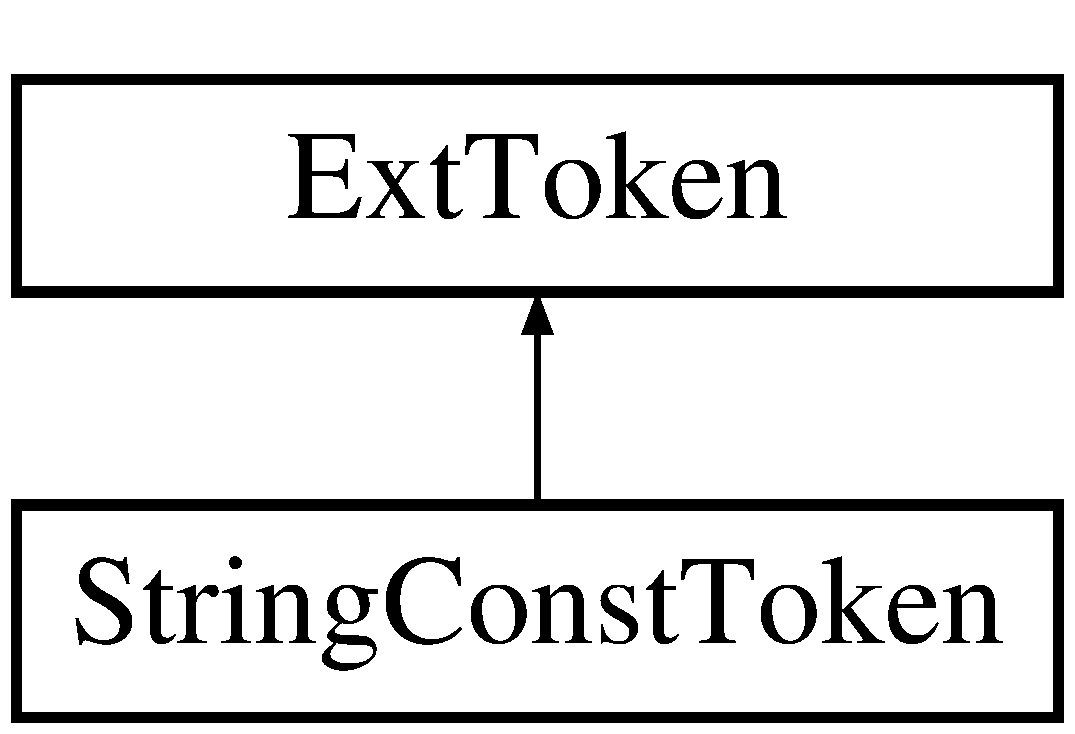
\includegraphics[height=2.000000cm]{classStringConstToken}
\end{center}
\end{figure}
\subsection*{Public Member Functions}
\begin{DoxyCompactItemize}
\item 
\hypertarget{classStringConstToken_aba75cdaef187138a572ba49a5c279fcf}{{\bfseries String\-Const\-Token} (\hyperlink{classParser}{Parser} $\ast$p, \hyperlink{classToken}{Token} $\ast$t)}\label{classStringConstToken_aba75cdaef187138a572ba49a5c279fcf}

\item 
\hypertarget{classStringConstToken_a4767bba84d30289ab31d501f240b80fb}{\hyperlink{classParseResult}{Parse\-Result} {\bfseries nud} ()}\label{classStringConstToken_a4767bba84d30289ab31d501f240b80fb}

\item 
\hypertarget{classStringConstToken_a6343169471a6cb6e422496f2f640691f}{std\-::string {\bfseries description} ()}\label{classStringConstToken_a6343169471a6cb6e422496f2f640691f}

\end{DoxyCompactItemize}
\subsection*{Additional Inherited Members}


The documentation for this class was generated from the following file\-:\begin{DoxyCompactItemize}
\item 
ext\-Token.\-h\end{DoxyCompactItemize}

\hypertarget{classToken}{\section{Token Class Reference}
\label{classToken}\index{Token@{Token}}
}
\subsection*{Public Member Functions}
\begin{DoxyCompactItemize}
\item 
\hypertarget{classToken_a087251cfeb05246cc96c92880a3d80ad}{{\bfseries Token} (std\-::string lex, token\-Type type)}\label{classToken_a087251cfeb05246cc96c92880a3d80ad}

\item 
\hypertarget{classToken_a529e83dd830006aaa3a73369eba215d7}{{\bfseries Token} (std\-::string lex, token\-Type type, \hyperlink{classToken}{Token} $\ast$next)}\label{classToken_a529e83dd830006aaa3a73369eba215d7}

\end{DoxyCompactItemize}
\subsection*{Public Attributes}
\begin{DoxyCompactItemize}
\item 
\hypertarget{classToken_abbff29ede445ed4a8520580f12490832}{std\-::string {\bfseries lexeme}}\label{classToken_abbff29ede445ed4a8520580f12490832}

\item 
\hypertarget{classToken_a11b4722b5e4023d234d2017126de378b}{token\-Type {\bfseries terminal}}\label{classToken_a11b4722b5e4023d234d2017126de378b}

\item 
\hypertarget{classToken_a32f24a25af788c192e5b387dc8d67914}{\hyperlink{classToken}{Token} $\ast$ {\bfseries next}}\label{classToken_a32f24a25af788c192e5b387dc8d67914}

\end{DoxyCompactItemize}


The documentation for this class was generated from the following files\-:\begin{DoxyCompactItemize}
\item 
scanner.\-h\item 
scanner.\-cpp\end{DoxyCompactItemize}

\hypertarget{classTrueKwdToken}{\section{True\-Kwd\-Token Class Reference}
\label{classTrueKwdToken}\index{True\-Kwd\-Token@{True\-Kwd\-Token}}
}
Inheritance diagram for True\-Kwd\-Token\-:\begin{figure}[H]
\begin{center}
\leavevmode
\includegraphics[height=2.000000cm]{classTrueKwdToken}
\end{center}
\end{figure}
\subsection*{Public Member Functions}
\begin{DoxyCompactItemize}
\item 
\hypertarget{classTrueKwdToken_aec070f83a6b91ed35a41e24dfd301b17}{{\bfseries True\-Kwd\-Token} (\hyperlink{classParser}{Parser} $\ast$p, \hyperlink{classToken}{Token} $\ast$t)}\label{classTrueKwdToken_aec070f83a6b91ed35a41e24dfd301b17}

\item 
\hypertarget{classTrueKwdToken_ad86f05acb9483438db153eab44aa6dac}{\hyperlink{classParseResult}{Parse\-Result} {\bfseries nud} ()}\label{classTrueKwdToken_ad86f05acb9483438db153eab44aa6dac}

\item 
\hypertarget{classTrueKwdToken_af4dbe740f06e6928a436d06349af67a9}{std\-::string {\bfseries description} ()}\label{classTrueKwdToken_af4dbe740f06e6928a436d06349af67a9}

\end{DoxyCompactItemize}
\subsection*{Additional Inherited Members}


The documentation for this class was generated from the following file\-:\begin{DoxyCompactItemize}
\item 
ext\-Token.\-h\end{DoxyCompactItemize}

\hypertarget{classVariableNameToken}{\section{Variable\-Name\-Token Class Reference}
\label{classVariableNameToken}\index{Variable\-Name\-Token@{Variable\-Name\-Token}}
}
Inheritance diagram for Variable\-Name\-Token\-:\begin{figure}[H]
\begin{center}
\leavevmode
\includegraphics[height=2.000000cm]{classVariableNameToken}
\end{center}
\end{figure}
\subsection*{Public Member Functions}
\begin{DoxyCompactItemize}
\item 
\hypertarget{classVariableNameToken_a804403db425122d1c8d40fd2c6172439}{{\bfseries Variable\-Name\-Token} (\hyperlink{classParser}{Parser} $\ast$p, \hyperlink{classToken}{Token} $\ast$t)}\label{classVariableNameToken_a804403db425122d1c8d40fd2c6172439}

\item 
\hypertarget{classVariableNameToken_a6e775ad5b8c2eafd2e2a185ab90b1f27}{\hyperlink{classParseResult}{Parse\-Result} {\bfseries nud} ()}\label{classVariableNameToken_a6e775ad5b8c2eafd2e2a185ab90b1f27}

\item 
\hypertarget{classVariableNameToken_a54bc3a78736e5c967dc4b1c58e66135b}{std\-::string {\bfseries description} ()}\label{classVariableNameToken_a54bc3a78736e5c967dc4b1c58e66135b}

\end{DoxyCompactItemize}
\subsection*{Additional Inherited Members}


The documentation for this class was generated from the following file\-:\begin{DoxyCompactItemize}
\item 
ext\-Token.\-h\end{DoxyCompactItemize}

\hypertarget{classVarname}{\section{Varname Class Reference}
\label{classVarname}\index{Varname@{Varname}}
}


{\ttfamily \#include $<$A\-S\-T.\-h$>$}

Inheritance diagram for Varname\-:\begin{figure}[H]
\begin{center}
\leavevmode
\includegraphics[height=3.000000cm]{classVarname}
\end{center}
\end{figure}
\subsection*{Public Member Functions}
\begin{DoxyCompactItemize}
\item 
\hypertarget{classVarname_a717889d6da22e437f71468c26eedd79d}{{\bfseries Varname} (std\-::string \-\_\-lexeme)}\label{classVarname_a717889d6da22e437f71468c26eedd79d}

\item 
\hypertarget{classVarname_a88ccb6c2760c23a28be071d6b7fe0496}{std\-::string {\bfseries unparse} ()}\label{classVarname_a88ccb6c2760c23a28be071d6b7fe0496}

\end{DoxyCompactItemize}


\subsection{Detailed Description}
This class is for a variable name expression 

The documentation for this class was generated from the following files\-:\begin{DoxyCompactItemize}
\item 
A\-S\-T.\-h\item 
A\-S\-T.\-cpp\end{DoxyCompactItemize}

%--- End generated contents ---

% Index
\newpage
\phantomsection
\addcontentsline{toc}{chapter}{Index}
\printindex

\end{document}
